\part{Applications}

大多数人都在应用程序层与计算机打交道。通过对计算机各个分层的抽象,即使用户对应用程序层下的各个计算层一无所知,也可以使用应用软件。在我们的生活中,计算机被我们用来管理和分析数据,其效用几乎无处不在。当今计算机应用主要分为以下五个方面:信息系统、人工智能、模拟、计算机辅助设计和嵌入式系统等。

我们使用信息系统来组织和管理数据,从运动统计数据到薪资表等,收银机和ATM都有大型的信息系统支持(PIN码验证和余额查询等)。

从技术上说信息系统就是为了支持决策和组织控制而收集(或获取)、处理、存储、分配信息的一组相互关联的组件。除了支持决策、协作和控制,信息系统也可用来帮助经理和工人分析解决问题,使复杂性可视化,以及创造新的产品,从商业角度看,一个信息系统是一个用于解决环境提出的挑战的,基于信息技术的组织管理方案。

一个基于计算机的信息系统是以计算机软件、硬件、存储和电信等技术为核心的人机系统。信息系统应用中又以电子制表软件和数据库管理系统的应用最为突出,它们广泛地应用于我们组织和分析数据的过程中。

电子制表软件是用单元格来组织数据和用于计算新值的公式的应用软件,用行列标号可以引用单元格。单元格可以存放基本数据或公式,这些公式通常会引用其它单元格中的值,还会使用内置函数来计算结果。此外,公式还可以使用一个单元格范围内的数据。如果单元格中存放的是公式,那么真正显示的是公式计算出的值。

对于电子数据表中的公式,避免循环引用(两个或多个单元格的计算结果要互相依赖)很重要。

电子数据表具有多功能性和可扩展性,它们适用于多种不同的情况,能够对变化动态地做出响应。如果电子数据表中的值被改变了,相关的公式会自动重新计算,生成最新的结果。如果给电子数据表添加了行或列,那么公式的范围也会被立刻校正,因此电子数据表尤其适用于模拟假设分析,其中的假设值将被不断修改,以了解对系统其他数据的影响。

数据库管理系统包括存储数据的物理文件、支持数据访问和修改的软件以及指定数据库的逻辑布局的数据库模式。关系模型是目前最常用的数据库模型,结构化查询语言(SQL)是查询和操作关系数据库的标准语言。

数据库管理系统用表组织数据,表由记录(对象)构成,记录由域(属性)构成。每个表会被指派一个(或一组)键域,键的值唯一标识了表中的每个元素。

数据库元素之间的关系可以用新的表来表示,这个表也可以有自己的属性。关系表并不是重复其他表的数据,而是存储数据库记录的关键值,以便需要的时候能够查找详细的数据。

人工智能(Artificial Intelligence,AI)是计算的一个子学科,它向人们展示了计算的未来。AI也有自己专用的数据管理技术。同时,AI也是应用新技术来解决问题的途径,对许多类型的应用程序的开发都有影响。

在现代工业应用中,飞机制造商通过建立风洞来研究新的飞行器设计中的机翼周围的气流,同样在汽车工业中也会通过风洞来验证气流对车体设计的影响。

飞行模拟器是一种模型,可以再现飞行器对驾驶员所做的动作的反应,可以使驾驶员能够在进入驾驶舱之前学习正确控制飞行器,每一个驾驶员都要在飞行模拟器中花费大量的时间。在新的超级市场的规划方案定稿之前,可以通过运行计算机模拟程序,根据预测的顾客流量,以协助确定需要多少个收银台。

风洞、飞行模拟器和上述的计算机程序都是模型。用一种模型表示现象、对象或状况的技术叫做模拟。通过支持模拟技术的理论,在实际应用中还有更多具体的例子,包括预测天气的模型等。

计算机辅助设计(CAD)和嵌入式系统(Embedded System)是另外两种计算的应用。建筑师、工程师和设计师可以用CAD系统构建结构和产品的计算机模型。嵌入式系统可以理解为大型系统中专用于执行有限功能的计算机系统。

\chapter{信息管理}

在计算机科学中,把信息定义为原始事实,把数据定义为以方便计算机使用的方式组织起来的信息。信息系统(Information System)一般定义为帮助我们组织和分析数据的软件。

根据Laudon的MIS阶层与系统间的关系,有六大系统支持四个阶层:

\begin{compactitem}
\item 作业控制阶层——主要为DPS(Data Processing System,数据处理系统)或称TPS(Transaction Processing System,事务处理系统),负责收集各项可用于管理的数据,处理日常例行的事务数据,并产生报表以支持组织的作业控制活动,即MRS。

此类系统基本上是一种孤岛式的功能性文件系统,通常在信息系统发展的早期进行自动化时产生,可用来代替人工处理繁复的结构化数据。而此一阶层管理人员也可以应用DSS(Decision Support System,决策支持系统)完成相关决策工作。

\item 知识管理阶层——主要是KWS(Knowledge Work System,知识工作系统)与OS(Office System,办公室系统),负责累积知识与协助运用知识以提高组织的竞争力。而此一阶层管理人员也可以应用DSS完成相关决策工作。

\item 管理控制阶层——主要为MRS(Management Reporting System,管理报告系统),即狭义的MIS(Management Information System,管理信息系统),整合各个DPS所收集各项的数据,提供组织管理信息,反应部门现况,其内容通常是部门功能导向,用来解决各种结构性问题,可以产生综合摘要与例外报表以提供中阶管理人员使用,通常是一个大型的整合架构。而此一阶层管理人员也可以应用DSS完成相关决策工作。

\item 策略规划阶层——主要为EIS(Executive Information System,主管信息系统)或称ESS(Executive Support System,主管支持系统),提供组织状况,支持高层决策,是一种计算机化系统,支持、提供高阶主管所需的决策信息,并支持主管规划、分析和沟通所需的能力,重点在于追踪、控制与沟通。又分成组之状况报导系统与人际沟通支持系统。而此一阶层管理人员也可以应用DSS完成相关决策工作。


\end{compactitem}

DSS是一种协助人类做决策的信息系统,协助用户规划与分析各种行动方案,常用试误的方法进行,通常是以交谈式的方法来解决半结构性或非结构性的问题,但其所强调的是支持而非代替人类进行决策。任何应用程序都是管理数据的,不过有一些程序则是采用特定的结构以特定的方式管理数据。还有一些专用应用程序则使用特定的技术解决问题,例如为支持人工智能需要的分析而提供的各种组织数据的方式。

然而,大多数情况都是一般性的,它们不需要特别考虑。我们只需要管理数据,捕捉数据间的关系。这种情况不需要任何特别的组织和处理,它们需要的是灵活的软件工具,能够让用户指示和管理数据的组织,并且具备用多种方式分析数据的能力。

两种最常用的一般信息系统是电子制表软件(Spreadsheet)和数据库管理系统。电子制表软件是用单元格(Cell)来组织数据和用于计算新值的公式的应用软件。在电子制表软件中采用可扩展的公式定义数据间的关系,适用于基础的数据分析。数据库管理系统适用于需要经常检索并且有组织的大量数据。

\chapter{电子制表软件}

电子制表软件使用带标签的单元格组织和分析数据,单元格可以存放基本数据或用于计算值的公式。存储在其中的数据既可以是文本,也可以是数字或其它特殊数据(如日期等)。

在电子制表软件中可以用行列标号引用电子数据表的单元格,通常用字母指定列,用数字指定行。因此,可以用诸如A1、C7和G45这样的标号来引用单元格。对于第26列之后的列,电子制表软件用两个字母作为列标号,所以,若单元格的标号是AA19,就代表第27列第19行。

通常,电子数据表有一个合理的最大行数,如256或者65536。另外,大多数电子制表软件一般会把多个表组合在一个大的交互系统中,来管理大量的数值和计算。

下面来看一个小型的实例,以说明电子数据表的基本原理。假设我们搜集了几个星期以来向一组辅导老师求助的学生的数据,假设现在我们掌握了5个星期以来每周分别向三位辅导老师(Hal、Amy和Frank)求助的学生的人数。我们要对这些数据执行一些基本的分析,下面的就是收集的电子数据表。



\begin{table}
\centering
\begin{tabular}{|m{10pt}|m{25pt}|m{25pt}|m{25pt}|m{25pt}|m{25pt}|m{25pt}|m{25pt}|m{25pt}|}
\hline
	&A	&B	&C	&D	&E	&F	&G	&H\\
\hline
{\centering 1}	&	&	&	&	&	&	&	&	\\
\hline
{\centering 2}	&	&	&\multicolumn{4}{c|}{Tutor}	&	&	\\
\hline
{\centering 3}	&	&	&Hal&Amy&Frank&Total&Avg&		\\
\hline
{\centering 4}	&\multirow{5}{20pt}{\centering Week}&1&12&10&13&35&11.67	&\\ \cline{1-1} \cline{3-9}
%\hline
{\centering 5}	&	&2	&14&16&16&46&15.33&\\ \cline{1-1} \cline{3-9}
%\hline
{\centering 6}	&	&3	&10&18&13&41&13.67&\\ \cline{1-1} \cline{3-9}
%\hline
{\centering 7}	&	&4	&8&21&18&47&15.67&\\ \cline{1-1} \cline{3-9}
%\hline
{\centering 8}	&	&5	&15&18&12&45&15.00&\\ \cline{1-1} \cline{3-9}
\hline
{\centering 9}	&	&Total&59&83&72&214&71.33&\\
\hline
{\centering 10}	&	&Avg&11.80&16.60&14.40&42.80&14.27&\\
\hline
{\centering 11}	&	&	&	&	&	&	&	&	\\
\hline
\end{tabular}
\end{table}

这个电子数据表除了具有其他数据外,还包括原始数据。例如单元格C4存放的是Hal在第1周辅导过的学生数。从C4到C8,存放的是Hal在这5周中每周辅导的学生数。同样地,Amy辅导的学生人数存放在D4到D8中,Frank辅导的学生人数存放在E4到E8中。可以把一行中的数据看作是意义相同的。

在单元格C9、D9和E9中,电子制表软件计算并显示出了每位辅导教师在5周中帮助过的学生的总数。在单元格C10、D10和E10中,还计算并显示出了每位辅导教师平均每周帮助的学生人次。同样地,从F4到F8显示了每周受到(所有辅导老师)帮助的学生的总数。从G4到G8是每周每位老师辅导的学生的平均数。

除了计算每位老师每周辅导的学生的总数和平均数外,电子制表软件还能计算其他的统计值。单元格F9是所有老师在5周中一共辅导过的学生人次。F10是所有老师平均每周辅导的学生人次,G9是每位老师5周中平均辅导的学生人次,最后,G10是每位老师平均每周辅导的学生人次。

第A列和第B列中的数据以及第2行和第3行中的数据只是用作标签,说明了其余单元格中存储的是什么值。这些标签只是为了便于人们理解,与计算无关。

电子制表软件允许用户控制单元格中的数据的外观和格式,可以设置数据的字体、样式、颜色和对齐方式等。对于实数值,可以设置显示多少位小数。在大多数电子制表软件中,还能够设置是否显示网格线、背景颜色或单元格的图案等。


\section{电子数据表公式}


使用电子数据表的好处在于易于修改和易于扩展,电子数据表的这种能力源于创建并存储在单元格中的公式。把公式存储在一个单元格中,这个单元格就会显示该公式的结果。因此,在查看电子数据表中的值时,很难分辨出单元格中的数据是直接输入的,还是通过公式计算出的。

下面将上述电子数据表中的公式标识出来,这些公式都是以等号(=)开头的。电子数据表就是通过这一点知道哪些单元格存放的是要计算的公式。

\begin{figure}[!h]
\centering
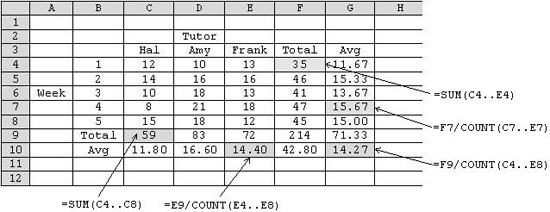
\includegraphics[scale=0.65]{xls_example.png}
\label{xls_example}
\end{figure}

电子数据表公式(通过列标号和行标号)引用了特定的单元格。在计算公式时,将用所引用的单元格中的值计算结果。每当电子数据表有变化,其中的公式都会被重新计算,所以表中的数据总是最新的。电子数据表是动态的,能对变化立即作出响应。

电子数据表中的公式可以利用标准符号(\verb|+、-、*、/|等)的基本数学运算,也可以使用电子制表软件内置的可用于公式的电子数据表函数(Spreadsheet Function)。

由于函数通常作用于一系列连续的单元格,因此电子制表软件提供了一种便捷的方式,即指定单元格的范围(range)。从语法上来讲,范围是由两个圆点及两端加两个单元格标号构成的。一个范围可以是一行中的一组单元格,如C4..E4,也可以是一列中的一组单元格,如C4..C8。此外,范围还可以是一个矩形块,指定了左上角的单元格标号和右下角的单元格标号,如C4..E8矩形块中包括了单元格C4到C8,D4到D8,E4到E8。总的来说,范围是用端点指定的一组连续单元格。

设计公式时,重要的一点是,除非特别适合,否则尽量避免在公式中使用常量。电子数据表中的原始数据发生变化,其中公式的值就会变化,公式自身也应该对插入和删除操作作出类似的响应。

电子制表软件通常会提供大量的函数。一些函数执行的是数学或统计运算、一般的金融计算或者是文本或日期的特殊运算。另一些函数则允许用户建立单元格间的逻辑关系。下表列出了一些常见的电子数据表函数。

\zihao{6}

\begin{table}[!h]
\begin{tabular}{|l|l|}
\hline
函数				&计算\\
\hline
SUM(val1,val2,...) 
\newline SUM(range)&指定的一组值的和\\
\hline
COUNT(val1,val2,...)
\newline COUNT(range)&非空单元格的个数\\
\hline
MAX(val1,val2,...)
\newline MAX(range)&指定的一组值中的最大值\\
hline
SIN(angle)	&指定角度的正弦值\\
\hline
PI()			&$\pi$的值\\
\hline
STDEV(val1,val2,...)
\newline STDEV(range)&指定的采样值的标准差\\
\hline
TODAY()	&今天的日期\\
\hline
LEFT(text,num\_chars)&指定文本的最左边的字符\\
\hline
IF(test,true\_val,false\_val)&如果test是true,则返回true\_val,否则返回false\_val\\
\hline
ISBLANK(value)&如果指定的值引用的是一个空单元格,则返回true\\
\hline
\end{tabular}
\end{table}

\zihao{5}


电子数据表的另一灵活之处是能够整行或整列地复制值或公式。复制公式时,单元格间的关系都将维持不变,因此很容易设置一整套类似的计算。在复制的公式中,对单元格的引用会被自动更新,以反映新的公式所在的行。



\section{循环引用}


电子数据表的公式可以有循环引用(Circular Reference),在计算结果时要错误地彼此依赖的一组公式,因而这种引用是不可能解决的,原因在于一个公式的结果始终是基于另一个公式的,反之亦然。例如,如果单元格B15中的公式如下:$$=\text{D22}+\text{D23}$$


而单元格D22中的公式是:$=\text{B15}+\text{B16}$

这就是一个循环引用。B15的结果要使用D22的值,而D22的结果又是由B15决定的。

循环引用通常不会这么明显,可能会涉及到多个单元格。下图展示了一个更复杂的情况,最终单元格A1的结果是由D13决定的,反之亦然。电子制表软件通常能探测出这些问题并提示错误信息。

\begin{table}[!h]
\centering
\begin{tabular}{|p{100pt}|p{200pt}|}
\hline
单元格	&内容\\
\hline
A1		&=B7*COUNT(F8..K8)\\
\hline
B7		&=A14+SUM(E40..E50)\\
\hline
E45		&=G18+G19-D13\\
\hline
D13	&=D12/A1\\
\hline
\end{tabular}
\end{table}


\section{电子数据表分析}


电子数据表的多功能性表现在用户可以决定其中的数据表示什么以及数据间的关系,因此电子数据表分析可以应用于任何领域,包括:

\begin{compactitem}
\item 跟踪销售情况
\item 分析运动统计数字
\item 维护学生的成绩单
\item 保存汽车的维修记录
\item 记录和总结旅行开销
\item 跟踪项目活动和日常安排
\item 计划股票购买
\end{compactitem}


一般说来,电子数据表的运算在商业领域的大量特定情况中是不可或缺的。

电子数据表的另一个特性是它的动态特性,一旦正确建立了电子数据表公式,那么计算会将数据的更改、添加或删除自动考虑在内。

电子数据表的动态特性还提供了进行模拟假设分析(what-if analysis)的功能。在使用中可以在电子数据表中设置一些假设,然后通过改变表示假设的值,以观察假设的变化对相关数据有什么影响,来质疑这些假设。

例如,假设我们创建了一个电子数据表用于估计举办一个研讨会的花费和潜在利润。我们可以输入参加者的人数、门票价格、资料费、会议室租金以及其他可能影响最终结果的数据,然后问自己假设分析的问题,看看随着各种条件的变化会出现哪些情况,问题如下:

\begin{compactitem}
\item 如果参加者人数减少了10\%将会怎么样?
\item 如果门票价格增加了\$5将会怎么样?
\item 如果把资料费减少一半将会怎么样?
\end{compactitem}



在问这些问题的同时改变相应的数据。如果已经正确建立了所有公式间的关系,那么每个改变都会立刻展示给我们其他数据发生了哪些变化。

商业分析师以各种方式标准化了这一过程,电子制表软件已经变成了一种主要的分析工具。成本效益分析、收支平衡计算以及预计销售价格都是通过组织电子数据表中的数据和公式来考虑适当的关系。

\chapter{数据库管理系统}


数据库(database)是一个以某种有组织的方式存储的数据集合,可以简单定义为结构化的数据集合。数据库通常是一个文件或一组文件,数据库是通过数据库管理系统(DBMS)创建和操纵的,从很大程度上说,数据库究竟是文件还是别的东西并不重要,因为我们并不直接访问数据库,数据库管理系统为我们访问数据库。

理解数据库的一个最简单的方法是将其想象为一个文件柜,此文件柜是一个存放数据的物理位置,不管数据是什么以及如何组织。

可能我们还没意识到,其实我们一直在使用数据库。当我们从电子邮件地址簿里查找名字时,或者使用搜索引擎时,都是在使用数据库。如果在工作中登录网络,也需要依靠数据库验证自己的用户名和密码。即使是在自动取款机上使用ATM卡,也要利用数据库进行PIN码验证和余额检查。

几乎所有复杂的数据库管理情况都要依靠下层的数据库和允许用户(人或程序)与之交互的支持结构。

数据库管理系统是一组软件和数据的组合,由下列几部分构成:

\begin{compactitem}
\item 物理数据库——存放数据的文件的集合;
\item 数据库引擎(engine)——支持对数据库内容的访问和修改的软件;
\item 数据库模式(schema)——存储在数据库中的数据的逻辑结构的规约。
\end{compactitem}

数据库管理系统包括存储数据的物理文件、支持数据访问和修改的软件以及指定数据库的逻辑布局的数据库模式。

数据库引擎与专用的数据库语言(比如SQL)交互,这种语言允许用户指定数据的结构,执行添加、修改、删除和更新数据的操作,以及查询数据库以获得指定的数据。

数据库模式提供了数据库中的数据的逻辑视图,独立于数据的物理存储方式。假设以一种有效的方式实现了数据库的物理结构,那么从数据库用户的观点来看,逻辑模式是更加重要的数据库视图,因为它展示了数据项之间的关系。

用户将先与数据库引擎软件交互,决定或修改数据库的模式。然后再与数据库引擎交互,访问和修改存储在磁盘上的数据库的内容。

下图展示了数据库管理系统的各个组件之间的关系。

\begin{figure}[!h]
\centering
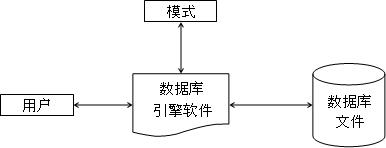
\includegraphics[scale=0.65]{db_example.png}
\label{db_example}
\end{figure}



\section{关系模型}


目前占统治地位的数据库管理模型是关系模型(Relational Model)。在关系型数据库管理系统(RDBMS)中,用表(table)组织数据项(item)和它们之间的关系(relation)。

表是记录(record)的集合。记录是域(field)的集合。数据库表的每个域都包括一个值。表中的每个记录都包含相同的域。

表中的记录又叫做数据库对象(object)或实体(entity),记录是构成一个数据库实体的相关的域的集合。记录中的域有时又叫做数据库对象的属性(attribute),是数据库记录中的一个值。

在将资料放入自己的文件柜时,并不是随便将它们扔进某个抽屉就完事了,而是在文件柜中创建文件,然后将相关的资料放入特定的文件中。在数据库领域中,这种文件就称为表。

表是一种结构化的文件,可以理解为某种特定类型的数据的结构化清单。表可以保存顾客清单、产品目录,或者其它信息清单。

这里关键的一点在于,存储在表中的数据是一种类型的数据或一个清单。绝不应该将顾客的清单与订单的清单存储在同一个数据库表中。这样做将使以后的检索和访问很困难。应该创建两个表,每个清单一个表。

表中的数据是按行(row)存储的,所保存的每个记录存储在自己的行内,如果将表想象为网格,网格中垂直的列为表列,水平行为表行。

例如,顾客表可以每行存储一个顾客,表中的行编号为记录的编号。

在很大程度上,行(row)和记录(record)这两个术语是可以互相交换使用的,但从技术上说,行才是正确的术语,行是表中的一个记录。

对记录对应,记录的域——列(column)组成了表,列中存储着表中某部分的信息,所有的表都是由一个或多个列组成的。

理解列的最好办法就是将数据库表想象为一个网格,网格中每一列存储着一条特定的信息。例如,在顾客表中,一个列存储着顾客编号,另一个列存储着顾客名,而地址、城市、州(或省)以及邮政编码全都存储在各自的列中。




\section{分解数据}


正确地将数据分解为多个列极为重要。例如,城市、州(或省)、邮政编码应该总是独立的列。通过把它分解开,才有可能利用特定的列对数据进行分类和过滤(如,找出特定州或省或特定城市的所有顾客)。如果城市和州(或省)组合在一个列中,则按州(或省)进行分类或过滤就会很困难。

数据库中每个列都有相应的数据类型(datatype),例如,如果列中存储的是数字,则相应的数据类型应该为数值类型。如果列中存储的是日期、文本、注释、金额等,则应该用恰当的数据类型规定出来。

数据类型定义(或限制)列可以存储的数据种类,例如,防止在数值字段中录入字符值等。数据类型还帮助正确地分类数据,并在优化磁盘使用方面起重要的作用。

数据类型及其名称是SQL不兼容的一个主要原因,虽然大多数数据类型得到一致的支持,但许多更为高级的数据类型却存在很大差异,甚至相同的数据类型在不同的DBMS中具有不同的名字,对此必须在创建表结构时记住这些差异。

数据库中的每个表都有一个用来标识自己的名字,此名字是唯一的。使表名成为唯一的,实际上是数据库名和表名等因素的组合,有的数据库还使用数据库拥有者的名字作为唯一名的组成部分。这表示,虽然在相同数据库中不能两次使用相同的表名,但在不同的数据库中却可以使用相同的表名。

考虑如下的数据库表,其中包含的是有关电影的信息。表中的每一行对应一条记录。表中的每条记录由相同的域构成,其中存储了特定的值。也就是说,每条电影记录都包括MovieId域、Title域、Genre域和Rating域,存放了这条记录特有的数据。数据库表都有一个名字,在这里的数据库表名是Movie。



\begin{figure}[!h]
\centering
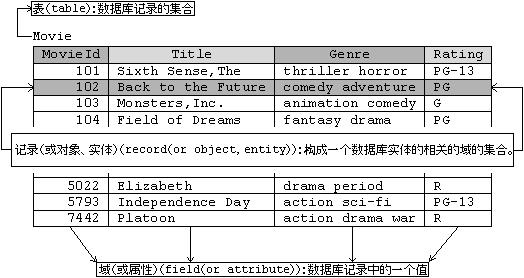
\includegraphics[scale=0.65]{table_example.png}
\label{table_example}
\end{figure}


通常,表中会有一个或多个域被标识为键(key)域\footnote{注:全国科学技术名词审定委员会审定的key在数据库中的对应名词为“键码”或“码”,不过对于key约定俗成的翻译是“键”。}。键域在表的所有记录中唯一标识了这个记录。也就是说,存储在表的每条记录的键域中的值必须是唯一的。在Movie表中,MovieId域是键的合理选择,因为两部电影可能重名,Genre域和Rating域也不适合作为键域。一般定义键(key)是在表的所有记录中唯一标识一个数据库记录的一个或多个域。


\section{主键}

唯一标识表中每行的这个列(或这组列)称为主键(Primary Key),主键用来表示一个特定的行。

没有主键,更新或删除表中特定行很困难,因为没有安全的方法保证只涉及相关的行,应该总是定义主键。

键域中的每个值都必须是唯一的,大多数DBMS可以自动生成这种域,以确保实体的唯一性。不过这并不要求键值是连续的。一个顾客表可以将顾客编号用于此目的,而包含订单的标可以使用订单ID,雇员表可以使用雇员ID或雇员社会保险号,同样地,上述Movie表中的最后三个实体包含的是截然不同的电影标识编号,只要它们是唯一的,MovieId域就可以作为域。

表中任何列都可以作为主键,只要它满足以下条件:

\begin{compactenum}
\item 任意两行都不具有相同的主键值;
\item 每个行都必须具有一个主键值(主键列不允许NULL值);
\item 主键列中的值不允许修改或更新;
\item 主键值不能重用(如果某行从表中删除,它的主键不能赋给以后的新行)。
\end{compactenum}

主键通常定义在表的一列上,但这并不是必需的,也可以一起使用多个列作为主键。在使用多个列作为主键时,上述条件必须应用到构成主键的所有列,所有列值的组合必须是唯一的(但单个列的值可以不唯一)。

另外还有一种非常重要的键,称为外键(Foreign Key)。

可以按照不同的方式排列数据库表中的记录。数据库表中的记录之间一般没有任何的内在关系。关系数据库表只是数据的逻辑视图,与底层的物理组织(记录是如何存储在存储器上)毫无关系。只有在查询数据库时,记录的排序才比较重要。例如要查询所有Rating是PG的电影,这时才可能会根据需要对查询的结果排序。

表具有一些特性,这些特性定义了数据在表中如何存储,如可以存储什么样的数据,数据如何分解,各部分信息如何命名等。描述表的这组信息就是所谓的模式(Schema),模式可以用来描述数据库中特定的表以及整个数据库(和其中表的关系)。
	
表的结构反映了它所表示的模式,也就是说,模式是表中的记录的属性的表达式。可以用下面的表达式表示上述数据库的模式:

\begin{lstlisting}[language=SQL]
Movie(MovieId : key,Title,Genre,Rating)
\end{lstlisting}
	
在模式表示法中还会说明每个域存储的数据的类型,如数字或文本等。此外还可能说明某个域可用的值的集合。例如在上述的数据库表中,可以说明Rating域的值只能是G、PG、PG-13、R或NC-17。整个数据库的模式由其中每个表的模式构成。

假设我们要创建一项电影租赁业务。除了出租的电影的清单外,还要创建一个客户信息表,我们使用Customer表存放了客户的信息。

\begin{figure}[!h]
\centering
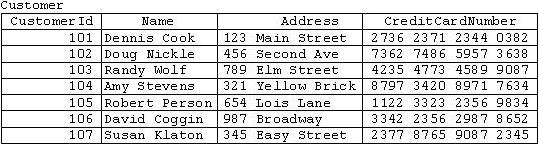
\includegraphics[scale=0.5]{table_customer.png}
\label{table_customer}
\end{figure}

与Movie表一样,Customer表也有一个键CustomerId域。某些CustomerId的值与MovieId的值相同,它们不会冲突。键的值只需要在同一个表中是唯一的。


正确地将数据分解为多个列极为重要,例如,城市、周、邮政编码应该总是独立的列。在真实的数据库中,最好把Name域分为FirstName和LastName两个域。此外,完整的地址也可能会根据实际情况的需要被分为几个部分,如City和State。通过分解数据才有可能利用特定的列对数据进行分类和过滤(例如,找出特定州或省或特定城市的所有顾客)。


Movie表和Customer表说明了如何用独立的表中的记录组织数据。而关系数据库管理系统的强大之处在于创建能把各个表从概念上联系起来的表,也就是说,数据库元素之间的关系可以用新的表表示,这个表也可以有自己的属性。

关系表并不是重复其他表的数据,而是存储数据库记录的关键值,以便需要的时候能够查找详细的数据。

%%
%%
%%
%%
%%
%%
%%
%%
\section{关系}


根据关系模型中的定义,记录表示的是独立的数据库对象,记录的域是这些对象的属性。可以创建一个记录来表示对象之间的关系,包括记录中的属性之间的关系。因此,可以用一个表来表示对象间的关系的集合。


继续深化上述电影出租的例子,要表示特定的客户租了哪些电影。由于“租用”是客户和电影之间的关系,所以可以把它表示为一个记录。租用的日期和到期日是这种关系的属性,于是可以创建一个新的数据库表Rents来表示当前被租走的电影的关系记录的集合。



\begin{figure}[!h]
\centering
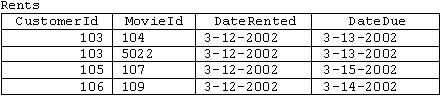
\includegraphics[scale=0.5]{table_rents.png}
\label{table_rents}
\end{figure}


Rents表包含有关关系中的对象(客户和电影)的信息和关系的属性。但是要注意的是,它并非包含客户和电影的所有信息。

在关系数据库中要尽量避免数据重复。例如,在Rents表中没有必要保存客户的名字和地址。Customer表已经存储了这些数据。当需要这些数据时,用存储在Rents表中的CustomerId来检索Customer表,查找该客户的详细信息即可。同样地,当需要有关电影的信息时,用MovieId检索Movie表即可。


在上述的Rents表中,CustomerId的值中出现了两次103,这说明同一个客户可以租借至少两部电影。


数据库表中的数据会根据需要被修改、添加、更新和删除。当给库存添加了电影或从中删除了电影时,Movie表中的记录都要更新。当有新客户的记录加入时,需要把它们添加到Customer表中。随着电影不断地被租出去或归还回来,还要添加或删除Rents表中的记录。


	
%%
%%
%%
%%
%%
%%
%%
%%
\section{通用产品代码}

使用通用产品代码(UPC)和与之关联的条形码是为了加速顾客在商店购买产品的速度,以及帮助跟踪库存。

\begin{figure}[!h]
\centering
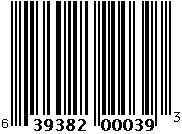
\includegraphics[scale=0.5]{universal_product_code.png}
\label{universal_product_code}
\end{figure}


UPC符号由机器能识别的条形码和人能识别的12位UPC编号组成。UPC编号的前6位数字是制造商的身份编号,接下来的5位数字是项目编号。每种类型的产品与同一产品的不同包装都有一个唯一的项目编号。因此,两升装的可口可乐和两升装的减肥可乐项目编号不同。最后一位UPC代码叫做校验数位,扫描器可以用它来确定扫描的UPC编号是否正确。校验数位是通过对UPC编号的其余数位的计算得来的。在读入UPC编号后,扫描器将对它执行运算,用校验数位进行验证。

针对某些产品,尤其是小产品,开发了新的UPC编号法,通过减少某些数位从而缩减了UPC编号。采用这种方法,可以减小整个UPC符号的大小。

注意,UPC编号并不存储产品的价格。当收银机(或者电子收款系统,POS)扫描一个产品时,它将使用UPC编号中的制造商编号和项目编号在数据库中检索该项目,而数据库则包含大量的产品信息,包括它的价格等。UPC中只保留基本的信息,这样不必更改产品的标签,就可以很容易的更改其他信息(比如价格等)。


%%
%%
%%
%%
%%
%%
%%
%%
%%
%%
%%
%%
%%
%%

\chapter{结构化查询语言}


结构化查询语言(Structured Query Language,SQL)是一种用于管理关系数据库的综合性数据库语言,包括指定数据库模式的语句和添加、修改、更新和删除数据库内容的语句。另外,还具有查询数据库以获取特定数据的功能。

SQL的原始版本是20世纪70年代IBM开发的Sequal语言。设计SQL的目的是很好地完成一项任务——提供一种从数据库中读写数据的简单有效的方法。

1986年,美国国家标准化组织(ANSI)发布了SQL标准,这是访问关系数据库的商用数据库语言的基础。

SQL有如下的优点:

\begin{compactitem}
\item SQL不区分大小写,空格被用作语句中的分隔符。
\item SQL不是某一个特定数据库专有的语言,几乎所有重要的DBMS都支持SQL。
\item SQL的语句全都是由有很强描述性的英语单词组成的。
\end{compactitem}

大多数DBMS以不自己完成文件分布的格式存储数据,这些SQL依赖于具体的DBMS运行。

许多DBMS提供商通过增加语句或指令,对SQL进行了扩展,这种扩展的目的是提供执行特定操作的额外功能或简化方法,虽然这种扩展很有用,但一般都是针对个别DBMS的,很少有两个以上的提供商支持这种扩展。

所有主要的DBMS,即使有自己的扩展,但这些扩展都支持ANSI SQL,比如PL/SQL、Transact-SQL等,其中PL/SQL是Oracle公司为其数据库产品开发的SQL扩展,Transact-SQL是微软与Sybase公司合作开发,适用于微软SQL Server和Sybase数据库。
%%
%%
%%
%%
%%
\section{ODBC}


ODBC(Open Database Connectivity)是一个为访问数据库提供的标准C接口,于1992年由SQL Access Group标准化,定义了一组用于访问数据库的标准C API。ODBC作为应用程序和数据库之间的中间件,使应用程序能与不同的后端数据库或基础数据库引擎交互。

ODBC本身不是数据库。但ODBC包装数据库,使所有数据库以一种一致和清晰定义的方式工作。它利用具有两种主要功能的软件驱动程序达到这一点。首先,它们封装数据库的本身特性或特色并对客户机隐藏它们。其次,它们提供一种常用的语言与这些数据库交互(在需要时进行转换)。ODB所用的语言就是SQL。

ODBC客户机应用程序并不直接与数据库交互,而是与ODBC数据源交互。数据源是一个逻辑数据库,它包括驱动程序(每种类型的数据库有自己的驱动程序)和如何连接到数据库的信息(文件路径、服务器名等)。

在定义了数据库源后,任何兼容ODBC的应用程序都可以使用这些数据源。ODBC并不针对具体的应用程序,它们针对的是系统。存在许多不同的ODBC程序版本,因此在设置具体的ODBC数据源时,应该密切注意具体的提示。

If you are using 64-bit Windows, be sure to check the documentation for how to configure the ODBC driver.  The short answer is:

\begin{compactenum}
\item Click Start / Run
\item Type \texttt{\%windir\%{\textbackslash}SysWOW64{\textbackslash}ODBCAD32.exe}
\item Continue configuring as normal.
\end{compactenum}


%%
%%
%%
%%
%%
\section{SQL的数学基础}


SQL的操作中混有代数,用于访问和操作关系表中的数据。这种代数是20世纪60年代末期由IBM的E.F.Codd定义的。SQL的基本操作包括:

\begin{compactitem}
\item select操作,用于识别表中的记录。
\item project操作,用于生成表列的子集。
\item 笛卡尔乘积操作,用于连接两个表的行。
\end{compactitem}

其他还有集合操作联合、求差、求交集、自然连接(笛卡尔乘积的子集)和除法操作。

编写SQL语句需要对基本的数据库设计有良好的理解。不知道什么信息存放在什么表中,表与表之间如何互相关联,以及行中数据如何分解,要编写高效的SQL是不可能的。

下面所用的表为一个假想的玩具销售商使用的订单录入系统的组成部分。这些表用来完成几项任务:

\begin{compactitem}
\item 管理供应商;
\item 管理产品目录;
\item 管理客户列表;
\item 录入客户订单;
\end{compactitem}

完成它们需要5个表(它们作为一个关系数据库设计的组成部分紧密关联)。虽然现实世界中的订单录入系统还记录了这里没有包括的大量数据(如工资和记账信息、发货追踪信息等)。不过,这些表确实示范了现实世界中会遇到的各种数据的组织和关系。

下面对5个表及每个表内的列名进行介绍。

\begin{compactenum}
\item Vendors表

Vendors表存储卖产品的供应商。每个供应商在这个表中有一个记录,供应商ID列(vend\_id)用于产品与供应商的匹配。

\begin{longtable}{|m{180pt}|m{180pt}|}
%%head
\hline
\multicolumn{2}{|c|}{Vendors表的列}
\tabularnewline\hline
列	&说明
\endhead
%%endhead

%%firsthead
\hline
\multicolumn{2}{|c|}{Vendors表的列}
\tabularnewline\hline
列	&说明
\endfirsthead
%%endfirsthead

%%foot
\multicolumn{2}{r}{}
\endfoot
%%endfoot

%%lastfoot
\endlastfoot
%%endlastfoot
\hline
vend\_id		&唯一的供应商ID\\
\hline
vend\_name		&供应商名\\
\hline
vend\_address	&供应商的地址\\
\hline
vend\_city		&供应商的城市\\
\hline
vend\_state		&供应商的州\\
\hline
vend\_zip		&供应商的邮政编码\\
\hline
vend\_country	&供应商的国家\\
\hline

\end{longtable}

所有表都应该有主键,这个表应该用vend\_id作为它的主键。

\item Products表

Products表包含产品目录,每行一个产品。每个产品有唯一的ID(prod\_id列),并且借助vend\_id(供应商的唯一ID)与供应商相关联。



\begin{longtable}{|m{180pt}|m{180pt}|}
%%head
\hline
\multicolumn{2}{|c|}{Products表的列}
\tabularnewline\hline
列	&说明
\endhead
%%endhead

%%firsthead
\hline
\multicolumn{2}{|c|}{Products表的列}
\tabularnewline\hline
列	&说明
\endfirsthead
%%endfirsthead

%%foot
\multicolumn{2}{r}{}
\endfoot
%%endfoot

%%lastfoot
\endlastfoot
%%endlastfoot
\hline
prod\_id		&唯一的产品ID\\
\hline
vend\_id		&产品供应商ID(关联到Vendors表的vend\_id列\\
\hline
prod\_name		&产品名\\
\hline
prod\_price		&产品价格\\
\hline
prod\_desc		&产品描述\\
\hline

\end{longtable}

所有表都应该有主键,这个表应该用prod\_id作为它的主键。

为实施引用完整性,应该在vend\_id上定义一个外键,关联它到Vendors的vend\_id列。

\item Customers表

Customers表存储所有客户信息。每个客户有唯一的ID(cust\_id列)。

\begin{longtable}{|m{180pt}|m{180pt}|}
%%head
\hline
\multicolumn{2}{|c|}{Customers表的列}
\tabularnewline\hline
列	&说明
\endhead
%%endhead

%%firsthead
\hline
\multicolumn{2}{|c|}{Customers表的列}
\tabularnewline\hline
列	&说明
\endfirsthead
%%endfirsthead

%%foot
\multicolumn{2}{r}{}
\endfoot
%%endfoot

%%lastfoot
\endlastfoot
%%endlastfoot
\hline
cust\_id		&唯一的客户ID\\
\hline
cust\_name	&客户名\\
\hline
cust\_address&客户的地址\\
\hline
cust\_city	&客户的城市\\
\hline
cust\_state	&客户的州\\
\hline
cust\_zip	&客户的邮政编码\\
\hline
cust\_country&客户的国家\\
\hline
cust\_contact&客户的联系名\\
\hline
cust\_email	&客户的联系电子邮件地址\\
\hline

\end{longtable}

所有表都应该有主键,这个表应该用cust\_id作为它的主键。

\item Orders表

Orders表存储客户订单(但不是订单细节)。每个订单唯一地进行编号(order\_num列)。Orders表按cust\_id列(关联到Customers表的客户唯一ID)关联到相应的客户。


\begin{longtable}{|m{180pt}|m{180pt}|}
%%head
\hline
\multicolumn{2}{|c|}{Orders表的列}
\tabularnewline\hline
列	&说明
\endhead
%%endhead

%%firsthead
\hline
\multicolumn{2}{|c|}{Orders表的列}
\tabularnewline\hline
列	&说明
\endfirsthead
%%endfirsthead

%%foot
\multicolumn{2}{r}{}
\endfoot
%%endfoot

%%lastfoot
\endlastfoot
%%endlastfoot
\hline
order\_num	&唯一的订单号\\
\hline
order\_date	&订单日期\\
\hline
cust\_id		&订单客户ID(关联到Customers表的cust\_id)\\
\hline
\end{longtable}

所有表都应该有主键。这个表应该用order\_num作为它的主键。

为实施引用完整性,应该在cust\_id上定义一个外键,关联它到Customers表的cust\_id列。

\item OrderItems表

OrderItems表存储每个订单中的实际物品,每个订单的每个物品一行。对于Orders表中的每一行,在OrderItems表中有一行或多行。每个订单物品由订单号加订单物品(第一个物品、第二个物品等)唯一标识。订单物品用order\_num列(关联到Orders表中订单的唯一ID)与其对应的订单相关联。此外,每个订单物品包含该物品的产品ID(把物品关联到Products表)。


\begin{longtable}{|m{180pt}|m{180pt}|}
%%head
\hline
\multicolumn{2}{|c|}{OrderItems表的列}
\tabularnewline\hline
列	&说明
\endhead
%%endhead

%%firsthead
\hline
\multicolumn{2}{|c|}{OrderItems表的列}
\tabularnewline\hline
列	&说明
\endfirsthead
%%endfirsthead

%%foot
\multicolumn{2}{r}{}
\endfoot
%%endfoot

%%lastfoot
\endlastfoot
%%endlastfoot
\hline
order\_num	&订单号(关联到Orders表的order\_num)\\
\hline
order\_item	&订单物品号(订单内的顺序)\\
\hline
prod\_id	&产品ID(关联到Products表的prod\_id)\\
\hline
quantity	&物品数量\\
\hline
item\_price	&物品价格\\
\hline

\end{longtable}

所有表都应该有主键。这个表应该用order\_num和order\_item作为它的主键。

为实施引用完整性,应该在order\_num和prod\_id上定义外键,关联order\_num到Orders的order\_num列,关联prod\_id到Products表的prod\_id列。

\end{compactenum}
%%
%%
%%
%%
%%
%%


\section{SQL数据类型}

SQL中数据类型是定义列中可以存储什么数据以及该数据实际怎样存储的基本规则。数据类型用于以下目的:

\begin{compactitem}
\item 数据类型允许限制可存储在列中的数据。例如,数值数据类型列只能接受数值。
\item 数据类型允许在内部更有效地存储数据。例如,可以用一种比文本串更简洁的格式存储数值和日期时间值。
\item 数据类型允许变换排序顺序。如果所有数据都作为串处理,则1位于10之前,而10又位于2之前(串以字典顺序排序,从左边开始比较,一次一个字符)。作为数值数据类型,数值才能正确排序。
\end{compactitem}

在设计表时,应该特别重视所用的数据类型。使用错误的数据类型可能会严重地影响应用程序的功能和性能。更改包含数据的列不是一件小事(而且这样做可能会导致数据丢失)。

任意两个DBMS都不是完全相同的,不同DBMS的数据类型可能有很大的不同。在不同的DBMS中,即使具有相同名称的数据类型也可能代表不同的东西。

\subsection{串数据类型}

最常用的数据类型是串数据类型。它们存储串,如名字、地址、电话号码、邮政编码等。有两种基本的串类型,分别为:定长串和变长串。

定长串接受长度固定的字符串,其长度是在创建表时指定的。例如,名字列可允许30个字符,而社会安全号列允许11个字符(允许的字符数目中包括两个破折号)。定长列不允许多于指定的字符数目。它们分配的存储空间和指定的一样多。因此,如果串Ben存储到30个字符的名字字段,则存储的是30个字符,缺少的字符用空格填充,或根据需要补为NULL。

变长串存储任意长度的文本(其最大长度随不同的数据类型和DBMS而变化)。有些变长数据类型具有最小的定长,而有些则是完全变长的。不管是哪种,只有指定的数据得到保存(额外的数据不保存)。

串数据类型分为定长串和变长串,有一个原因是出于性能的考虑。DBMS处理定长列远比处理变长列快得多。此外,许多DBMS不允许对变长列(或一个列的可变部分)进行索引。这也会极大地影响性能。

\begin{longtable}{|m{200pt}|m{180pt}|}
%%head
\hline
\multicolumn{2}{r}{}
\tabularnewline\hline
\endhead
%%endhead

%%firsthead
\caption{串数据类型}\\
\hline
\endfirsthead
%%endfirsthead

%%foot
\multicolumn{2}{r}{}
\endfoot
%%endfoot

%%lastfoot
\endlastfoot
%%endlastfoot
\hline
CHAR	&1~255个字符的定长串。它的长度必须在创建时规定。\\
\hline
NCHAR	&CHAR的特殊形式,用来支持多字节或Unicode字符(此类型的不同实现变化很大)\\
\hline
NVARCHAR&TEXT的特殊形式,用来支持多字节或Unicode字符(此类型的不同实现变化很大)\\
\hline
TEXT(也称为LONG,MEMO或VARCHAR)&变长文本\\
\hline
\end{longtable}

不管使用何种形式的串数据类型,串值都必须括在单引号内。

另外,当数值不是数值时,比如电话号码和邮政编码等,此时需要遵守的基本规则是:如果数值是计算(求和、平均等)中使用的数值,则应该存储在数值数据类型列中。如果作为字符串(可能包含数字)使用,则应该保存在串数据类型列中。

\subsection{数值数据类型}


数值数据类型存储数值。多数DBMS支持多种数值数据类型,每种存储的数值具有不同的取值范围。显然,支持的取值范围越大,所需存储空间越多。此外,有的数值数据类型支持使用十进制小数点(和小数),而有的则只支持整数。并非所有的DBMS都支持下列所列出的数值数据类型名称约定和描述。


\begin{longtable}{|m{180pt}|m{180pt}|}
%%head
\hline
\multicolumn{2}{r}{}
\tabularnewline\hline
\endhead
%%endhead

%%firsthead
\caption{数值数据类型}\\
\hline
\endfirsthead
%%endfirsthead

%%foot
\multicolumn{2}{r}{}
\endfoot
%%endfoot

%%lastfoot
\endlastfoot
%%endlastfoot
\hline
BIT 		&单个二进制位值,或者为0或者为1,主要用于开/关标志。\\
\hline
DECIMAL(或NUMERIC)&定点或精度可变的浮点值\\
\hline
FLOAT(或NUMERIC)&浮点值\\
\hline
INT(或INTEGER)&4字节整数值,支持从-2147483648~2147483647的数\\
\hline
REAL&4字节浮点值\\
\hline
SMALLINT&2字节整数值,支持从-32768~32767的数\\
\hline
TINYINT&1字节整数值,支持从0~255的数\\
\hline
\end{longtable}

与串数据类型不一样,数值不应该括在引号内。

多数DBMS支持一种用来存储货币值的特殊数值数据类型。一般记为MONEY或CURRENCY,这种数据类型基本上是特定取值范围的DECIMAL数据类型,只不过更适合存储货币值。

\subsection{日期和时间数据类型}

所有DBMS都支持用来存储日期和时间值的数据类型。与数值一样,多数DBMS都支持多种这种类型,每种具有不同的取值范围和精度。

\begin{longtable}{|m{180pt}|m{180pt}|}
%%head
\hline
\multicolumn{2}{r}{}
\tabularnewline\hline
\endhead
%%endhead

%%firsthead
\caption{日期和时间数据类型}\\
\hline
\endfirsthead
%%endfirsthead

%%foot
\multicolumn{2}{r}{}
\endfoot
%%endfoot

%%lastfoot
\endlastfoot
%%endlastfoot
\hline
DATE	&日期值\\
\hline
DATETIME(或TIMESTAMP)&日期时间值\\
\hline
SMALLDATETIME&日期时间值,精确到分(无秒或毫秒)\\
\hline
TIME&时间值\\
\hline
\end{longtable}

没有所有DBMS都理解的定义日期的标准方法。多数实现都理解诸如2004-12-30或Dec 30th,2004等格式,但即使这样,有的DBMS还是不理解它们。


\subsection{ODBC日期}


因为每种DBMS都有自己特定的日期格式,所以ODBC创建了自己的一种格式。在ODBC被使用时对每种数据库都起作用。

ODBC格式对于日期类似于\{d ‘2004-12-30’\},对于时间类似于\{t ‘21:46:29’\},而对于日期时间类似于\{ts ‘2004-12-30 21:46:29’\}。如果通过ODBC使用SQL,应该以这种方式格式化日期和时间。


\subsection{二进制数据类型}

二进制数据类型是最不具有兼容性的数据类型。与其他所有数据类型(它们具有特定的用途)不一样,二进制数据类型可包含任何数据,包括二进制信息,如图像、多媒体、字处理文档等。

\begin{longtable}{|m{180pt}|m{180pt}|}
%%head
\hline
\multicolumn{2}{r}{}
\tabularnewline\hline
\endhead
%%endhead

%%firsthead
\caption{二进制数据类型}\\
\hline
\endfirsthead
%%endfirsthead

%%foot
\multicolumn{2}{r}{}
\endfoot
%%endfoot

%%lastfoot
\endlastfoot
%%endlastfoot
\hline
BINARY	&定长二进制数据(最大长度从255字节到8000字节,有赖于具体的实现)\\
\hline
LONG RAW&变长二进制数据,最大2GB\\
\hline
RAW(某些实现为BINARY)&定长二进制数据,最多255字节\\
\hline
VARBINARY&变长二进制数据(最大长度一般在255字节到8000字节间变化,依赖于具体的实现)\\
\hline
\end{longtable}



\section{SQL保留字}

SQL是由关键字组成的语言,关键字是一些用于执行SQL操作的特殊词汇。在命名数据库、表、列和其他数据库对象时,一定不要使用这些关键字。因此,关键字是一定要保留的。下面列出的是主要的DBMS中最常用的保留字。

\begin{compactitem}
\item 关键字随不同的DBMS而变化,并非所列出的关键字都被所有DBMS采用;
\item 许多DBMS扩展了SQL保留字,使其包含专门用于实现的术语。多数DBMS专用的关键字未列出;
\item 为保证以后的兼容性和可移植性,应避免使用这些可能的保留字,即使它们不是当前使用的DBMS的保留字也是如此。
\end{compactitem}

\begin{longtable}{m{120pt}m{120pt}m{120pt}}
\rowcolors{1}{White}{Lavender}
%%head
\endhead
%%endhead

%%firsthead
\caption{SQL保留字}\\
\endfirsthead
%%endfirsthead

%%foot
\endfoot
%%endfoot

%%lastfoot
\endlastfoot
%%endlastfoot
ABORT						&ABSOLUTE		&	ACTION					\\
ACTIVE						&ADD				&AFTER\\
ALL							&ALLOCATE		&	ALTER\\
ANALYZE					&AND				&ANY\\
ARE							&AS				&	ASC\\
ASCENDING					&ASSERTION		&	AT\\
AUTHORIZATION			&AUTO				&AUTO-INCREMENT\\
AUTOING					&AVG				&BACKUP\\
SEFORE						&BEGIN				&BETWEEN\\
BIGINT						&BINARY			&	BIT\\
BLOB						&BOOLEAN			&BOTH\\
BREAK						&BROWSE			&BULK\\
BY							&BYTES				&CACHE\\
CALL						&CASCADE			&CASCADED\\
CASE						&CAST				&CATALOG\\
CHANGE					&CHAR				&CHARACTER\\
CHARACTER\_LENGTH		&CHECK			&	CHECKPOINT\\
CLOSE						&CLUSTER			&CLUSTERED\\
COALESCE					&COLLATE			&COLUMN\\
COLUMNS					&COMMENT		&	COMMIT\\
COMMITTED				&COMPUTE			&COPUTED\\
CONDITIONAL				&CONFIRM			&CONNECT\\
CONNECTION				&CONSTRAINT		&CONSTRAINS\\
CONTAINING				&CONTAINS		&	CONTAINSTABLE\\
CONTINUE					&CONTROROW		&CONVERT\\
COPY						&COUNT			&	CREATE\\
CROSS						&CSTRING			&CUBE\\
CURRENT					&CURRENT\_DATE	&CURRENT\_TIME\\
CURRENT\_TIMESTAMP		&CURRENT\_USER	&CURSOR\\
DATABASE					&DATABASES		&	DATE\\
DATETIME					&DAY				&DBCC\\
DEALLOCATE				&DEBUG			&	DEC\\
DECIMAL					&DECLARE			&DEFAULT\\
DELETE						&DENY				&DESC\\
DESCENDING				&DESCRIBE			&DISCONNECT\\
DISK						&DISTINCT			&DISTRIBUTED\\
DIV							&DO				&	DOMAIN\\
DOUBLE					&DROP				&DUMMY\\
DUMP						&ELSE				&ELSEIF\\
ENCLOSED					&END				&ERRLVL\\
ERROREXIT					&ESCAPE			&	ESCAPED\\
EXCEPT						&EXCEPTION		&	EXEC\\
EXECUTE					&EXISTS			&	EXIT\\
EXPLAIN					&EXTEND			&EXTERNAL\\
EXTRACT					&FALSE				&FETCH\\
FIELD						&FIELDS			&	FILE\\
FILLFACTOR					&FILTER			&	FLOAT\\
FLOPPY						&FOR				&FORCE\\
FOREIGN					&FOUND			&	FREETEXT\\
FREETEXTTABLE				&FROM				&FULL\\
FUNCTION					&GENERATOR		&GET\\
GLOBAL					&GO				&	GOTO\\
GRANT						&GROUP			&	HAVING\\
HOLDLOCK					&HOUR				&IDENTITY\\
IF							&IN					&INACTIVE\\
INDEX						&INDICATOR		&	INFILE\\
INNER						&INOUT			&	INPUT\\
INSENSITIVE				&INSERT			&	INT\\
INTEGER					&INTERSECT		&	INTERVAL\\
INTO						&IS					&ISOLATION\\
JOIN						&KEY				&	KILL\\
LANGUAGE					&LAST				&LEADING\\
LEFT						&LENGTH			&LEVEL\\
LIKE						&LIMIT				&LINENO\\
LINES						&LISTEN			&	LOAD\\
LOCAL						&LOCK				&LOGFILE\\
LONG						&LOWER			&	MANUAL\\
MATCH						&MAX				&MERGE\\
MESSAGE					&MIN				&MINUTE\\
MIRROREXIT					&MODULE			&MONEY\\
MONTH						&MOVE				&NAMES\\
NATIONAL					&NATUAL			&NCHAR\\
NEXT						&NEW				&NO\\
NOCHECK					&NONCLUSTERED	&NONE\\
NOT						&NULL				&NULLIF\\
NUMERIC					&OF				&	OFF\\
OFFSET						&OFFSETS			&ON\\
ONCE						&ONLY				&OPEN\\
OPTION						&OR				&	ORDER\\
OUTER						&OUTPUT			&OVER\\
OVERFLOW					&OVERLAPS		&	PAD\\
PAGE						&PAGES			&	PARAMETER\\
PARTIAL					&PASSWORD		&	PERCENT\\
PERM						&PERMANENT		&PIPE\\
PLAN						&POSITION			&PRECISION\\
PREPARE					&PRIMARY			&PRINT\\
PRIOR						&PRIVILEGES		&	PROC\\
PROCEDURE				&PROCESSEXIT		&PROTECTED\\
PUBLIC						&PURGE			&	PAISERROR\\
READ						&READEXIT			&REAL\\
REFERENCES				&REGEXP			&RELATIVE\\
RENAME					&REPEAT			&	REPLACE\\
REPLICATION				&REQUIRE			&RESERV\\
RESERVING					&RESET				&RESTORE\\
RESTRICT					&RETAIN			&	RETURN\\
RETURNS					&REVOKE			&RIGHT\\
ROOLBACK					&ROLLUP			&ROWCOUNT\\
RULE						&SAVE				&SAVEPOINT\\
SCHEMA					&SECOND			&SECTION\\
SEGMENT					&SELECT			&	SENSITIVE\\
SEPARATOR					&SEQUENCE		&	SESSION\_USER\\
SET							&SETUSER			&SHADOW\\
SHARED					&SHOW			&	SHUTDOWN\\
SINGULAR					&SIZE				&SMALLINT\\
SNAPSHOT					&SOME				&SORT\\
SPACE						&SQL				&	SQLCODE\\
SQLERROR					&STABILITY			&STARTING\\
STARTS						&SATAISTICS		&	SUBSTRING\\
SUM						&SUSPEND			&TABLE\\
TABLES						&TAPE				&TEMP\\
TEMPORARY				&TEXT				&TEXTSIZE\\
THEN						&TIME				&TIMESTAMP\\
TO							&TOP				&	TRAILING\\
TRAN						&TRANSACTION	&	TRANSLATE\\
TRIGGER					&TRIM				&TRUE\\
TRUNCATE					&UNCOMMITTED	&	UNION\\
UNIQUE						&NUTIL				&UPDATE\\
UPDATETEXT				&UPPER			&	USAGE\\
USE							&USER				&USING\\
VALUE						&VALUES			&	VARCHAR\\
VARIABLE					&VARYING			&VERBOSE\\
VIEW						&VOLUME			&WAIT\\
WAITFOR					&WHEN			&	WHERE\\
WHILE						&WITH				&WORK\\
WRITE						&WRITETEXT		&	XOR\\
YEAR						&ZONE	&\\
\end{longtable}






\chapter{查询}


提交给数据库的信息请求称为查询(Query),select语句是查询的主要工具,它具有很多变体,能够访问数据库中的特定数据。

基本的select语句包括一个select从句、一个from从句和一个where从句。

\begin{lstlisting}[language=SQL]
select attribute-list from table-list where condition
\end{lstlisting}

select从句决定了要返回那些属性。from从句决定了使用哪个表进行查询。where从句限制了返回的数据。例如:

\begin{lstlisting}[language=SQL]
select Title from Movie where Rating = 'PG'
\end{lstlisting}

这个查询的结果是Movie表中所有Rating为PG的电影名的列表。如果不需要特殊的限制,可以省略where从句:

\begin{lstlisting}[language=SQL]
select Name,Address from Customer
\end{lstlisting}

这个查询返回的是Customer表中所有客户的名字和地址。select从句中的星号(*)表示要返回选中的记录中的所有属性:

\begin{lstlisting}[language=SQL]
select * from Movie where Genre like '%action%'
\end{lstlisting}

这个查询返回的是Movie表中Genre属性包含单词action的记录的所有属性。SQL中的like操作执行的是字符串的模式匹配,符号\%与任何字符串都匹配。

select语句还可以用order从句指定查询结果的排序方法:

\begin{lstlisting}[language=SQL]
select * from Movie where Rating = 'R' order by Title
\end{lstlisting}

这个查询返回的是Rating为R的电影的所有属性,按照电影名的字母顺序排列。

SQL支持的select语句还有很多的变体,可以进一步细化查询。
%%
%%
%%
%%
%%
%%
\chapter{修改}


用SQL中的insert、update和delete语句,可以改变表中的数据,包括对数据库执行添加、修改和删除操作等。

insert语句可以给表添加一条新记录。每个insert语句都指定了新记录的属性值。例如:

\begin{lstlisting}[language=SQL]
insert into Customer values(9876,'John Smith',
'602 Greenbriar Court','2980 3423 5564 8796')
\end{lstlisting}
	
	这个语句将在Customer表中插入一条指定了属性的新记录。
	
	update语句可以改变表中的一条或多条记录的值。例如:
	
\begin{lstlisting}[language=SQL]
update Movie set Genre='thriller drama' where title='Unbreakable'
\end{lstlisting}
	
	这个语句将把电影Unbreakable的Genre属性改为thriller drama。
	
	delete语句可以删除表中与指定的条件匹配的所有记录。例如,如果要删除Movie表中所有Rating为R的电影,可以使用下列delete语句:
	
\begin{lstlisting}[language=SQL]
delete from Movie where Rating = 'R'
\end{lstlisting}

	
	与select语句一样,insert、update和delete语句也有很多变体。
%%
%%
%%
%%
%%
%%
%%
\chapter{SQL语句}

在书写SQL语句和阅读语句语法时,应该记住以下约定:

\begin{compactitem}
\item |符号用来指出几个选择中的一个,因此,NULL | NOT NULL表示或者给出NULL或者给出NOT NULL。
\item 包含在方括号中的关键词或子句(如[like this])是可选的。
\item SQL基本语句的语法几乎对所有DBMS都有效。
\end{compactitem}

\section{ALTER TABLE}

ALTER TABLE用来更新已存在的表的结构。为了创建表,应该使用CREATE TABLE。

\begin{lstlisting}[language=SQL]
ALTER TABLE
(
	ADD | DROP column datatype [NULL | NOT NULL] [CONSTRAINS],
	ADD | DROP column datatype [NULL | NOT NULL] [CONSTRAINS],
	. . .
);
\end{lstlisting}


\section{COMMIT}

COMMIT用来将事务处理写到数据库。

\begin{lstlisting}[language=SQL]
COMMIT [TRANSACTION];
\end{lstlisting}

\section{CREATE INDEX}

CREATE INDEX用于在一个或多个列上创建索引。

\begin{lstlisting}[language=SQL]
CREATE INDEX indexname 
ON tablename (column, . . . );
\end{lstlisting}

\section{CREATE PROCEDURE}

CREATE PROCEDURE用于创建存储过程。Oracle的语法稍有不同。

\begin{lstlisting}[language=SQL]
CREATE PROCEDURE procedurename [parameters] [options] 
AS SQL statement;
\end{lstlisting}


\section{CREATE TABLE}

CREATE TABLE用于创建新数据库表。为更新已经存在的表的结构,使用ALTER TABLE。

\begin{lstlisting}[language=SQL]
CREATE TABLE tablename
(
	column datatype [NULL | NOT NULL] [CONSTRAINS],
	column datatype [NULL | NOT NULL] [CONSTRAINS],
	. . .
);
\end{lstlisting}

\section{CREATE VIEW}

CREATE VIEW用来创建一个或多个表上的新视图。

\begin{lstlisting}[language=SQL]
CREATE VIEW viewname AS
SELECT columns, . . .
FROM tables, . . .
[WHERE . . .]
[ORDER BY . . .]
[HAVING . . .];
\end{lstlisting}

\section{DELETE}

DELETE从表中删除一行或多行。

\begin{lstlisting}[language=SQL]
DELETE FROM tablename
[WHERE . . .];
\end{lstlisting}

\section{DROP}

DROP永久地删除数据库对象(表、视图、索引等)。

\begin{lstlisting}[language=SQL]
DROP INDEX | PROCEDURE | TABLE | VIEW indexname | procedurename | tablename | viewname;
\end{lstlisting}

\section{INSERT}

INSERT给表增加行。

\begin{lstlisting}[language=SQL]
INSERT INTO tablename [(columns, . . .)]
VALUES(values, . . .);
\end{lstlisting}

\section{INSERT SELECT}

INSERT SELECT插入SELECT的结果到一个表。

\begin{lstlisting}[language=SQL]
INSERT INTO tablename [(columns, . . .)]
SELECT columns, . . . FROM tablename, . . .
[WHERE . . .];
\end{lstlisting}


\section{ROLLBACK}


ROLLBACK用于撤销一个事务处理块。

\begin{lstlisting}[language=SQL]
ROLLBACK [TO savepointname];
\end{lstlisting}

或者:

\begin{lstlisting}[language=SQL]
ROLLBACK TRANSACTION;
\end{lstlisting}


\section{SELECT}

SELECT用于从一个或多个表(视图)中检索数据。

\begin{lstlisting}[language=SQL]
SELECT columnname, . . .
FROM tablename, . . .
[WHERE . . .]
[UNION . . .]
[GROUP BY . . .]
[HAVING . . .]
[ORDER BY . . .];
\end{lstlisting}


\section{UPDATE}

UPDATE更新表中一行或多行。

\begin{lstlisting}[language=SQL]
UPDATE tablename
SET columnname = value, . . .
[WHERE . . .];
\end{lstlisting}
%%
%%
%%
%%
%%
%%
%%
%%
%%
%%
%%
%%
%%
%%
\chapter{SQL基本操作}

SQL是一种语言而不是应用程序,SQL语句是由简单的英语单词构成的,这些单词称为关键字,每个SQL语句都是由一个或多个关键字(keyword)构成的。

关键字是作为SQL组成部分的保留字,关键字不能用作表或列的名字。

SQL语句由子句(clause)构成,有些子句是必需的,而有的可选。一个子句通常由一个关键字加上所提供的数据构成。
%%
%%
%%
%%
\section{检索数据}

SELECT语句用于从一个或多个表中检索信息。为了使用SELECT检索表数据,必须至少给出两条信息——想选择什么,以及从什么地方选择。


%%
%%
%%
\subsection{检索单个列}


\begin{lstlisting}[language=SQL]
SELECT prod_name
FROM Products;
\end{lstlisting}



上述语句从Products表中检索一个名为prod\_name的列。所需的列名在SELECT关键字之后给出,FROM关键字指出从其中检索数据的表名。

SQL关键字不区分大小写,因此SELECT和select是相同的。在处理SQL语句时,其中所有空格都被忽略,因此SQL语句可以在一行上给出,也可以分成许多行。

检索数据时,如果没有明确排序查询结果,则返回的数据的顺序没有特殊意义,此时数据没有过滤(过滤将得出结果集的一个字节),也没有排序。不同的DBMS返回数据的顺序可能是数据被添加到表中的顺序,也可能不是。只要返回相同数目的行,就是正常的。

SQL语句一般返回原始的、无格式的数据。数据的格式化是一个表示问题,而不是一个检索问题。因此,数据表示一般在显示该数据的应用程序中规定。一般很少使用实际检索出的数据(没有应用程序提供的格式)。

多条SQL语句必须以分号(;)分隔,多数DBMS不需要在单条SQL语句后加分号。但特定的DBMS可能必须在单条SQL语句后加分号。这条规则的例外是Sybase Adaptive Serer,它不允许SQL语句以分号结束。

习惯上,SQL语句分成多行编写,而且对所有SQL关键字使用大写,而对所有列和表名使用小写。
%%
%%
%%
%%
\subsection{检索多个列}

要想从一个表中检索多个列,使用相同的SELECT语句,唯一的不同是必须在SELECT关键字后给出多个列名,列名之间必须以逗号(,)分隔,但最后一个列名后不加。如果在最后一个列名后加了逗号,将出现错误。

\begin{lstlisting}[language=SQL]
SELECT prod_id,prod_name,prod_price
FROM Products;
\end{lstlisting}
%%
%%
%%
%%
\subsection{检索所有列}


除了指定所需的列外,SELECT语句还可以检索所有的列而不必逐个列出它们。这可以通过在实际列名的位置使用星号(*)通配符来达到。

\begin{lstlisting}[language=SQL]
SELECT *
FROM Products;
\end{lstlisting}

给定通配符(*),则返回表中所有列。列的顺序一般(但并不总是)是列在表定义中出现的物理顺序。但SQL数据很少这样(通常,数据返回给一个根据需要进行格式化或表示的应用程序)。严格说来,这不应该造成什么问题。

使用通配符有一个大优点,由于不明确指定列名(星号匹配每个列),所以能检索出名字未知的列。
%%
%%
%%
%%
%%
\section{排序检索数据}

使用SELECT语句的ORDER BY子句,可以根据需要排序检索出的数据。
%%
%%
%%
%%
%%
%%
%%
\subsection{排序数据}

使用SELECT语句检索出的语句并不是以纯粹的随机方式显示的。如果不排序,数据一般将以它在底层表中出现的顺序显示。这可以是数据最初添加到表中的顺序。但是,如果数据后来进行过更新或删除,则此顺序将会受到DBMS重用回收存储空间的影响。因此,如果不明确控制的话,不能(也不应该)依赖该排序顺序。

关系数据库设计理论认为,如果不明确规定排序顺序,则不应该假定检索出的数据的顺序有意义。

为了明确地排序用SELECT语句检索出的数据,可以使用ORDER BY子句。ORDER BY子句取一个或多个列的名字,据此对输出进行排序。

\begin{lstlisting}[language=SQL]
SELECT prod_name
FROM Products
ORDER BY prod_name;
\end{lstlisting}

通常,ORDER BY子句中使用的列将是为显示所选择的列。但是,实际上并不一定要这样,用非检索的列排序数据是完全合法的。

在指定一条ORDER BY子句时,应保证它是SELECT语句中最后一条子句。该子句的次序不对将会出现错误信息。
%%
%%
%%
%%
%%
\subsection{按多个列排序}

实际的应用情景可能是,如果要显示雇员清单,可能希望按姓和名排序(首先按姓排序,然后在每个姓中再按名排序)。如果多个雇员具有相同的姓,这样做很有用。

为了按多个列排序,简单指定列名,列名之间用逗号分开即可(和检索多个列的形式一样)。


\begin{lstlisting}[language=SQL]
SELECT prod_id,prod_price,prod_name
FROM Products
ORDER BY prod_price,prod_name;
\end{lstlisting}

重要的是理解在按多个列排序时,排序的顺序完全按所规定的进行。对于上述例子中的输出,仅在多个行具有相同的prod\_price值时才对产品按prod\_name进行排序。如果prod\_price列中所有的值都是唯一的,则不会按prod\_name排序。

%%
%%
%%
\subsection{按列位置排序}



除了能用列名指出排序顺序外,ORDER BY还支持按相对列位置进行排序。

\begin{lstlisting}[language=SQL]
SELECT prod_id,prod_price,prod_name
FROM Products
ORDER BY 2,3;
\end{lstlisting}

这里,SELECT清单中指定的是选择列的相对位置而不是列名。ORDER 2表示按SELECT清单中的第二个列,prod\_price列进行排序。ORDER BY 2,3表示先按prod\_price,再按prod\_name进行排序。

按列位置排序的好处在于不用重新输入列名。但它也有缺点。首先,不明确给出列名增加了错用列名排序的可能性。其次,在对SELECT清单进行更改时容易错误地对数据排序(忘记对ORDER BY子句做相应的改动)。最后,如果进行排序的列不在SELECT清单中,显然不能使用这项技术。

显然,当根据没有出现在SELECT清单中的列进行排序时,不能采用按列位置排序技术。但是,如果有必要,可以混合匹配使用实际列名和相对列位置。
%%
%%
%%
%%
\subsection{指定排序方向}

数据排序不限于升序排序(从A到Z),这只是默认的排序顺序,还可以使用ORDER BY子句以降序(从Z到A)顺序排序。为了进行降序排序,必须指定DESC关键字。

\begin{lstlisting}[language=SQL]
SELECT prod_id,prod_price,prod_name
FROM Products
ORDER BY prod_price DESC;
\end{lstlisting}

如果打算用多个列排序,下面的例子以降序排序产品(最贵的在最前面),然后再对产品名排序。

\begin{lstlisting}[language=SQL]
SELECT prod_id,prod_price,prod_name
FORM Products
ORDER BY prod_price DESC,prod_name;
\end{lstlisting}

DESC关键字只应用到直接位于其前面的列名。在上例中,只对prod\_price列指定DESC,对prod\_name列不指定,因此,prod\_price列以降序排序,而prod\_name列(在每个价格内)仍然按标准的升序排序。

如果需要在多个列上进行降序排序,必须对每个列指定DESC关键字。

DESC为DESCENDING的缩写,这两个关键字是通用的。DESC的反面是ASC(或ASCENDING),在升序排序时可以指定它。但实际上,ASC没有多大用处,因为升序是默认的(如果既不指定ASC也不指定DESC,则假定为ASC)。

另外,在对文本性的数据进行排序时,A与a相同吗?a位于B之前还是位于Z之后?这些问题不是数据库理论问题,结果依赖于数据库如何设置。

在字典(dictionary)排序顺序中,A被视为与a相同,这是大多数DBMS的默认行为。但是,许多DBMS允许DBA在需要时改变这种行为(如果数据库中包含大量外语字符,可能必须这么做)。

这里,关键的问题是,如果确实需要改变这种排序顺序,用简单的ORDER BY子句做不到,必须请求DBA的帮助。
%%
%%
%%
%%
\section{过滤数据}

可以通过使用SELECT语句的WHERE子句指定搜索条件来过滤数据。数据也可以在应用层过滤。为此目的,SQL的SELECT语句为客户机应用检索出超过实际所需的数据,然后客户机代码对返回数据循环处理,以提取出需要的行。

通常,这种实现并不令人满意。因此,对数据库进行了优化,以便快速有效地对数据进行过滤。让客户机应用(或开发语言)处理数据库的工作将会极大地影响应用的性能,并且使所创建的应用完全不具备可伸缩性。此外,如果在客户机上过滤数据,服务器不得不通过网络发送多余的数据,这导致网络带宽的浪费。
%%
%%
%%
%%
%%
\subsection{使用WHERE子句}

数据库表一般包含大量的数据,很少需要检索表中所有行。通常只会根据特定操作或报告的需要提取表数据的子集。只检索所需数据需要指定搜索条件(search criteria),搜索条件也称为过滤条件(filter condition)。

在SELECT语句中,数据根据WHERE子句中指定的搜索条件进行过滤。WHERE子句在表明(FROM子句)之后给出。

\begin{lstlisting}[language=SQL]
SELECT prod_name,prod_price
FROM Products
WHERE prod_price = 3.49;
\end{lstlisting}

这个例子采用相等测试,检查一个列是否具有指定的值,据此进行过滤,但是SQL允许做的事情不仅仅是相等测试。SQL支持的条件操作符(operator)如下:

\begin{longtable}{|m{180pt}|m{180pt}|}
%%head
\hline
\multicolumn{2}{|c|}{WHERE子句操作符}
\tabularnewline\hline
列	&说明
\endhead
%%endhead

%%firsthead
\hline
\multicolumn{2}{|c|}{WHERE子句操作符}
\tabularnewline\hline
列	&说明
\endfirsthead
%%endfirsthead

%%foot
\multicolumn{2}{r}{}
\endfoot
%%endfoot

%%lastfoot
\endlastfoot
%%endlastfoot
\hline
操作符	&说明\\
\hline
=		&等于\\
\hline
<\/>		&不等于\\
\hline
!\/=		&不等于\\
\hline
<		&小于\\
\hline
<\/=	&小于等于\\
\hline
!\/<		&不小于\\
\hline
>		&大于\\
\hline
>\/=	&大于等于\\
\hline
!\/>		&不大于\\
\hline
BETWEEN&在指定的两个值之间\\
\hline
IS NULL&为NULL值\\
\hline
\end{longtable}

上述列出的某些操作符是冗余的(如<\/>与!\/=相同,!\/<(不小于)相当于>\/=(大于等于))。并非所有的DBMS都支持这些操作符,需要参考具体说明文档。

另外,PostgreSQL对传递给SQL语句的值具有严格的管理条件,特别是对于十进制数的列所用的数。为使上面的例子正常运行,需要在WHERE子句中包含类型,明确告诉PostgreSQL,3.49是一个合法的数。为此,应该将=3.49替换为=decimal `3.49'。

\begin{lstlisting}[language=SQL]
SELECT prod_name,prod_price
FROM Products
WHERE prod_price = Decimal '3.49';
\end{lstlisting}

PostgraSQL在7.3版本之后才取消对语句格式的这种限制。

在同时使用ORDER BY和WHERE子句时,应该让ORDER BY位于WHERE之后,否则将会产生错误。

%%
%%
%%
%%
%%
\subsection{检查单个值}

\begin{lstlisting}[language=SQL]
SELECT prod_name,prod_price
FROM Products
WHERE prod_price < 10;
\end{lstlisting}
%%
%%
%%
%%
%%
\subsection{不匹配检查}

\begin{lstlisting}[language=SQL]
SELECT vend_id,prod_name
FROM Products
WHERE vend_id <> 'DLL01';
\end{lstlisting}

其中,单引号用来限定字符串。如果将值与串类型的列进行比较,则需要限定引号。用来与数值列进行比较的值不用引号。

\begin{lstlisting}[language=SQL]
SELECT vend_id,prod_name
FROM Products
WHERE vend_id !='DLL01';
\end{lstlisting}

!\/=和<\/>通常可以互换使用,但是,并非所有DBMS都支持这两种不等于操作符,例如Microsoft Access就支持后者而不支持前者。


%%
%%
%%
%%
%%
%%
%%
%%
\subsection{范围值检查}


为了检查某个范围的值,可以使用BETWEEN操作符,其语法与其他WHERE子句的操作符稍有不同,因为它需要两个值,即范围的开始值和结束值。例如,BETWEEN操作符可以用来检索价格在5美元和10美元之间的或日期在指定的开始日期和结束日期之间的所有产品。


\begin{lstlisting}[language=SQL]
SELECT prod_name,prod_price
FROM Products
WHERE prod_price BETWEEN 5 AND 10;
\end{lstlisting}

在使用BETWEEN时,必须指定两个值——所需范围的低端值和高端值。这两个值必须用AND关键字分隔。BETWEEN匹配范围中所有的值,包括指定的开始值和结束值。
%%
%%
%%
%%
%%
\subsection{空值检查}

在创建表时,表设计人员可以指定其中的列是否可以不包含值。在一个列不包含值时,称其为包含空值NULL。

注意,NULL(无值,no value)与字段包含0、空字符串或仅仅包含空格是不同的。

SELECT语句有一个特殊的WHERE子句,可以用来检查具有NULL值的列,这个子句就是IS NULL子句。

\begin{lstlisting}[language=SQL]
SELECT prod_name
FROM Products
WHERE prod_price IS NULL;
\end{lstlisting}

这条语句返回没有价格(空prod\_price字段,而不是价格0)的所有产品。


%%
%%
%%
%%
\section{高级数据过滤}

许多DBMS扩展了标准的操作符表,提供了更高级的过滤选择。而通过组合WHERE子句可以建立功能更强的更高级的搜索条件。
%%
%%
%%
%%
\subsection{组合WHERE子句}

为了进行更强的过滤控制,SQL允许给出多个WHERE子句,这些子句可以两种方式使用,即:AND子句的方式或OR子句的方式使用。

这里AND或OR操作就是用来联结或改变WHERE子句中的子句的关键字,也称为逻辑操作符(logical operator)。
%%
%%
%%
%%
\subsection{AND操作符}


为了通过不止一个列进行过滤,可以使用AND操作符给WHERE子句附加条件。

\begin{lstlisting}[language=SQL]
SELECT prod_id,prod_price,prod_name
FROM Products
WHERE vend_id = ‘DLL01’ AND prod_price <= 4;
\end{lstlisting}

这条SQL语句检索由供应商DLL01且价格小于等于4美元的所有产品的名称和价格。这条SELECT语句中的WHERE子句包含两个条件,并且用AND关键字联结它们。AND指示DBMS只返回满足所有给定条件的行。如果某个产品由供应商DLL01制造,但它的价格高于4美元,则不检索它。类似,如果产品价格小于4美元,但不是由指定供应商制造的也不被检索。

因此,WHERE子句中的AND关键字用来指示检索满足所有给定条件的行。
%%
%%
%%
\subsection{OR操作符}


OR操作符与AND操作符不同,它指示DBMS检索匹配任一条件的行。事实上,许多DBMS在OR WHERE子句的第一个条件满足的情况下,不再计算第二个条件(在第一个条件满足时,不管第二个条件是否满足,相应的行都被检索出来)。

\begin{lstlisting}[language=SQL]
SELECT prod_name,prod_price
FROM Products
WHERE vend_id = ‘DLL01’ OR vend_id = ‘BRS01’;
\end{lstlisting}

这条SQL语句检索由任一个指定供应商制造的所有产品的产品名和价格。OR操作符指示DBMS匹配任一条件而不是同时匹配两个条件。如果这里使用的是AND操作符,则没有数据返回。
%%
%%
%%
%%
%%
\subsection{计算次序}

WHERE子句可以包含任意数目的AND和OR操作符。允许两者结合以进行复杂和高级的过滤。但是,组合AND和OR带来了一定的问题。

例如需要列出价格为10美元(含)以上且由DLL01或BRS01制造的所有产品。下面的SELECT语句使用AND和OR操作符的组合建立了一个WHERE子句。

\begin{lstlisting}[language=SQL]
SELECT prod_name,prod_price
FROM Products
WHERE vend_id = ‘DLL01’ OR vend_id = ‘BRS01’ 
AND prod_price >= 10;
\end{lstlisting}

显然,返回结果却未按预期的进行过滤。原因在于计算的次序。SQL在处理OR操作符前,优先处理AND操作符。当DBMS处理上述SQL语句时,它理解为由供应商BRS01制造的任何为10美元以上的产品,或者由供应商DLL01制造的任何产品,而不管其价格如何。换句话说,由于AND在计算次序中优先级更高,操作符被错误地组合了。

这个问题的解决方法是使用圆括号明确地分组相应的操作符。


\begin{lstlisting}[language=SQL]
SELECT prod_name,prod_price
FROM Products
WHERE (vend_id = ‘DLL01’ OR vend_id = ‘BRD01’) 
AND prod_price >=10;
\end{lstlisting}

圆括号具有较AND或OR操作符更高的计算次序。DBMS首先过滤圆括号内的OR条件。这时,SQL语句变成了选择由供应商DLL01或BRS01制造的且价格都在10美元(含)以上的任何产品。

任何时候使用包含AND和OR操作符的WHERE子句,都应该使用圆括号明确地分组操作符。不要过分依赖默认计算次序,即使它确实是想要的东西也是如此。使用圆括号没有什么坏处,它能消除歧义。
%%
%%
%%
%%
%%
\subsection{IN操作符}

IN操作符用来指定条件范围,范围中的每个条件都可以进行匹配。IN取合法值的由逗号分隔的清单,全都括在圆括号中。

\begin{lstlisting}[language=SQL]
SELECT prod_name,prod_price
FROM Products
WHERE vend_id IN (‘DLL01’ , ‘BRS01’)
ORDER BY prod_name;
\end{lstlisting}

这条SQL语句检索供应商DLL01和BRS01制造的所有产品,IN操作符后跟由逗号分隔的合法值清单,整个清单必须括在圆括号中。

WHERE子句中用IN来指定要匹配值的清单,功能与OR相当。下面的SQL语句完成与上面的例子相同的工作:


\begin{lstlisting}[language=SQL]
SELECT prod_name,prod_price
FROM Products
WHERE vend_id = ‘DLL01’ OR vend_id = ‘BRS01’
ORDER BY prod_name;
\end{lstlisting}

为什么要使用IN操作符?其优点为:

\begin{compactitem}
\item 在使用长的合法选项清单时,IN操作符的语法更清楚且更直观;
\item 在使用IN时,计算的次序更容易管理(因为使用的操作符更少);
\item IN操作符一般比OR操作符清单执行更快;
\item IN操作符的最大优点是可以包含其它SELECT语句,使得能够更动态地建立WHERE子句。
\end{compactitem}


%%
%%
%%
%%
%%
\subsection{NOT操作符}

WHERE子句中的NOT操作符有且只有一个功能,那就是否定它之后所跟的任何条件。因为NOT从不自己使用(它总是与其它操作符一起使用),它的语法与其他操作符有所不同。与其他操作符不一样,NOT可以用在要过滤的列前,而不仅是在其后。

\begin{lstlisting}[language=SQL]
SELECT prod_name
FROM Products
WHERE NOT vend_id = ‘DLL01’
ORDER BY prod_name;
\end{lstlisting}

使用NOT操作符后,DBMS会匹配其后的条件之外的其他所有东西。上述SQL语句也可以使用<>操作符来完成。

\begin{lstlisting}[language=SQL]
SELECT prod_name
FROM Products
WHERE NOT vend_id <> ‘DLL01’
ORDER BY prod_name;
\end{lstlisting}

在简单的SQL语句中,使用NOT没有什么优势。但是在复杂的子句中,NOT是非常有用的。例如,在与IN操作符联合使用时,NOT使找出与条件列表不匹配的行非常简单。

MySQL不支持上述描述的NOT格式,在MySQL中,NOT只用来否定EXISTS(如NOT EXISTS)。
%%
%%
%%
%%
%%
%%
%%
\section{用通配符进行过滤}

前面介绍的所有操作符都是针对已知值进行过滤的。不管是匹配一个还是多个值,测试大于还是小于已知值,或者检查某个范围的值,共同点是过滤中使用的值都是已知的。但是,这种过滤方法并不是任何时候都好用。例如,怎样搜索产品名中包含文本bean bag的所有产品?用简单的比较操作符肯定不行,必须使用通配符(wildcard)。

通配符是用来匹配值的一部分的特殊字符,利用通配符可以创建比较特定数据的搜索模式(search schema)。在上面的例子,可以通过通配符构造一个通配符搜索模式,找出产品名中任何位置出现bean bag的产品。

通配符本身实际是SQL的WHERE子句中有特殊含义的字符,由子面值、通配符或两者结合就构成了搜索模式。

SQL支持几种通配符,为在搜索子句中使用通配符,必须使用LIKE操作符。LIKE指示DBMS,后跟的搜索模式利用通配符匹配而不是直接相等匹配进行比较。

操作符在它作为谓词(predicate)时不是操作符,从技术上说,LIKE是谓词而不是操作符。

通配符搜索只能用于文本字段(串),非文本数据类型字段不能使用通配符搜索。
%%
%%
%%
%%
%%
%%
%%
%%
\subsection{百分号通配符}

最常使用的通配符是百分号(\%),在搜索串中,\%表示任何字符出现任意次数。例如,为了找出所有以词Fish起头的产品,可发布以下SELECT语句:

\begin{lstlisting}[language=SQL]
SELECT prod_id,prod_name
FROM Products
WHERE prod_name LIKE ‘Fish%’;
\end{lstlisting}

这里使用了搜索模式‘Fish\%’,执行这条子句时,将检索任意以Fish起头的词。\%告诉DBMS接受Fish之后的任意字符,不管它有多少字符。如果使用Microsoft Access,需要使用*而不是\%。

另外,根据DBMS的不同及其配置,搜索可以是区分大小写的。如果区分大小写,‘fish\%’与Fish bean bag toy将不匹配。

通配符可在搜索模式中任意位置使用,并且可以使用多个通配符。下面的例子使用两个通配符,它们位于模式的两端:

\begin{lstlisting}[language=SQL]
SELECT prod_id,prod_name
FROM Products
WHERE prod_name LIKE ‘%bean bag%’;
\end{lstlisting}

搜索模式 ‘\%bean bag\%’表示匹配任何位置包含文本bean bag的值,而不论它之前或之后出现什么字符。

通配符也可以出现在搜索模式的中间,虽然这样做不太有用。下面的例子找出以F起头以y结尾的所有产品。

\begin{lstlisting}[language=SQL]
SELECT prod_name
FROM Products
WHERE prod_name LIKE ‘F%y’;
\end{lstlisting}

重要的是要注意到,除了一个或多个字符外,\%还能匹配0个字符。\%代表搜索模式中给定位置的0个、1个或多个字符。

许多DBMS,包括Microsoft Access,都用空格来填补字段的内容。例如,如果希望某列有50个字符,而存储的文本为Fish bean bag toy(17个字符),则为填满该列需要在文本后附加33个空格。这样做一般对数据及其使用没有影响,但是可能对上述SQL语句有负面影响。子句WHERE prod\_name LIKE ‘F\%y’只匹配以F开头,以y结尾的prod\_name。如果值后面跟空格,则不是以y结尾,所以Fish bean bag toy就不会检索出来。一个简单的解决办法是给搜索模式再加一个\%号:‘F\%y\%’还匹配y之后的字符(或空格)。更好的解决方法是用函数去掉空格。


%%
%%
%%
%%
%%
\subsection{下划线(\_)通配符}

下划线(\_)通配符的用途与\%一样,但下划线只匹配单个字符而不是多个字符。如果使用的是Microsoft Access,需要使用?而不是\_。

\begin{lstlisting}[language=SQL]
SELECT prod_id,prod_name
FROM Products
WHERE prod_name LIKE ‘__ inch teddy bear’;
\end{lstlisting}

此WHERE子句中的搜索模式给出了后面跟有文本的两个通配符。结果只显示匹配搜索模式的行。比如8 inch teddy bear产品没有匹配,因为搜索模式要求匹配两个通配符而不是一个。而下面的SQL语句则可以正确返回8 inch teddy bear结果。

\begin{lstlisting}[language=SQL]
SELECT prod_id,prod_name
FROM Products
WHERE prod_name LIKE ‘% inch teddy bear’;
\end{lstlisting}

与\%能匹配0个字符不一样,\_总是匹配一个字符,不能多也不能少。

%%
%%
%%
%%
\subsection{方括号([ ])通配符}

方括号([ ])通配符用来指定一个字符集,它必须匹配指定位置(通配符的位置)的一个字符。注意,并不是所有DBMS都支持用来创建集合的[],集合只为Microsoft Access、SQL Server和Sybase Adaptive Server所支持。

例如,为找出所有名字以J或M起头的联系人,可如下查询:

\begin{lstlisting}[language=SQL]
SELECT cust_contact
FROM Customers
WHERE cust_contact LIKE ‘[JM]%’
ORDER BY cust_contact;
\end{lstlisting}

此语句的WHERE子句中的模式为 ‘[JM]\%’,此搜索模式使用了两个不同的通配符。[JM]匹配任何以方括号中字母开头的联系人名,它也只能匹配单个字符。因此,任何多于一个字符的名字都不匹配。[JM]之后的\%通配符匹配第一个字符之后的任意数目的字符,返回所需结果。

此通配符可以用前缀字符\^{}(脱字号)来否定。例如,下面的查询匹配不以J或M起头的任意联系人名(与前一个例子相反):

\begin{lstlisting}[language=SQL]
SELECT cust_contact
FROM Customers
WHERE cust_contact LIKE ‘[^JM]%’
ORDER BY cust_contact;
\end{lstlisting}

如果使用的是Microsoft Access,需要用!而不是\^{}来否定一个集合,因此使用的是[!JM]而不是[\^{}JM]。

当然,也可以使用NOT操作符得出相同的结果。\^{}的唯一优点是在使用多个WHERE子句时简化语法:

\begin{lstlisting}[language=SQL]
SELECT cust_contact
FROM Customers
WHERE NOT cust_contact LIKE ‘[JM]%’
ORDER BY cust_contact;
\end{lstlisting}

%%
%%
%%
%%
%%
%%
\subsection{使用通配符的技巧}

并非所有DBMS都支持方括号([ ])通配符。虽然SQL的通配符很有用,但这种功能是有代价的,即:通配符搜索的处理一般要比前面讨论的其它搜索所花时间更长。下面是一些使用通配符时要记住的技巧:

\begin{compactitem}
\item 不要过分使用通配符。如果其它操作符能达到相同的目的,应该使用其它操作符;
\item 在确实需要使用通配符时,除非绝对有必要,否则不要把它们用在搜索模式的开始处。把通配符置于搜索模式的开始处,搜索起来是最慢的。
\item 仔细注意通配符的位置。如果放错地方,可能不会返回想要的数据。
\end{compactitem}


%%
%%
%%
%%
\section{创建计算字段}

存储在数据库表中的数据一般不是应用程序所需要的格式。下面举几个例子:


\begin{compactitem}
\item 如果想显示公司名,同时还想显示公司的地址,但这两个信息一般包含在不同的表列中。
\item 城市、州(或省)和邮政编码存储在不同的列中(应该这样),但邮件标签打印程序却需要把它们作为一个恰当格式的字段检索出来。
\item 列数据是大小写混合的,但报表程序需要把所有数据按大写表示出来。
\item 物品订单表存储物品的价格和数量,但不需要存储每个物品的总价格(用价格乘以数量即可)。为打印发票,需要物品的总价格。
\item 需要根据表数据进行总数、平均数计算或其他计算。
\end{compactitem}

对于上述每个需求,存储在表中的数据都不是应用程序所需要的。我们需要直接从数据库中检索出转换、计算或格式化过的数据;而不是检索出数据,然后再在客户机应用程序中重新格式化。

要实现上述需求,就需要计算字段(field)。计算字段并不实际存在于数据库表中,而是运行时在SELECT语句内创建的。

字段基本上与列的意思相同,不过数据库列一般称为列,而术语字段通常用在计算字段的连接上。

只有数据库知道SELECT语句中哪些列是实际的表列,哪些列是计算字段。从客户机(如应用程序)的角度看来,计算字段的数据是以与其它列的数据相同的方式返回的。

注意,可在SQL语句内完成的许多转换和格式化工作都可以直接在客户机应用程序内完成。但一般来说,在数据库服务器上完成这些操作比在客户机中完成要快得多,因为DBMS是设计来快速有效地完成这种处理的。
%%
%%
%%
%%
%%
%%
\subsection{拼接字段}


为了说明如何使用计算字段,下面通过拼接(concatenate)字段创建由两列组成的标题的例子。
Vendors表包含供应商名和位置信息。假如要生成一个供应商报表,需要在格式化的名称(域位置)中列出供应商的位置。此报表需要单个值,而表中数据存储在两个列vend\_name和vend\_country中。此外,需要用括号将vend\_country括起来,这些信息都没有存储在数据库表中。

解决办法是通过拼接字段把两个列拼接起来。在SQL的SELECT语句中,可使用一个特殊的操作符来拼接两个列,可以是加号(+)或两个竖杠(||),有赖于具体的DBMS。

\begin{lstlisting}[language=SQL]
SELECT vend_name + ‘(’ + vend_country + ‘)’
FROM Vendors
ORDER BY vend_name;
\end{lstlisting}

下面是相同的语法,但使用的是||语法:

\begin{lstlisting}[language=SQL]
SELECT vend_name || ‘(’ || vend_country || ‘)’
FROM Vendors
ORDER BY vend_name;
\end{lstlisting}

上述SQL语句连接以下元素:

\begin{compactitem}
\item 存储在vend\_name列中的名字;
\item 包含一个空格和一个开圆括号的串;
\item 存储在vend\_country列中的国家;
\item 包含一个空格和一个闭圆括号的串。
\end{compactitem}


从输出中可以看到,SELECT语句返回包含上述四个元素的单个列(计算字段)。

MySQL不支持使用+或||的拼接,它使用CONCAT()函数把项表拼接起来。使用CONCAT()的SQL语句如下:

\begin{lstlisting}[language=SQL]
SELECT CONCAT(vend_name, ‘(’, vend_country, ‘)’)
FROM Vendors
ORDER BY vend_name;
\end{lstlisting}

MySQL确实支持||,但并不支持拼接。在MySQL中,||等同于操作符OR,而\&\&等同于操作符AND。

组合成一个计算字段的列之间一般会以空格填充,许多数据库(不是所有)保存填充为列宽的文本值。为正确返回格式化的数据,必须去掉这些空格。这可以使用SQL的RTRIM()函数来完成。

\begin{lstlisting}[language=SQL]
SELECT RTRIM(vend_name) + ‘(’ +RTRIM(vend_country) + ‘)’
FROM Vendors
ORDER BY vend_name;
\end{lstlisting}

下面是相同的语法,但使用的是||语法:

\begin{lstlisting}[language=SQL]
SELECT RTRIM(vend_name) || ‘(’ || RTRIM(vend_country) || ‘)’
FROM Vendors
ORDER BY vend_name;
\end{lstlisting}

RTRIM()函数去掉值右边的所有空格,通过使用RTRIM(),各个列都进行了整理。大多数DBMS都支持RTRIM()(用于去掉串右边空格)、LTRIM()(用于去掉串左边的空格)以及TRIM()(用于去掉串左右两边的空格)。
%%
%%
%%
%%
%%
%%
\subsection{使用别名}

使用计算字段时,拼接出来的新列是没有名字的,它只是一个值。如果仅是查看一下结果,这可以满足需求。但是,一个未命名的列不能用于客户机应用中,因为客户机没有办法引用它。为了解决这个问题,SQL支持列别名(alias)。

列别名是一个字段或值的替换名,用AS关键字赋予。

\begin{lstlisting}[language=SQL]
SELECT RTRIM(vend_name) + ‘(’ + RTRIM(vend_country) + ‘)’ AS vend_title
FROM Vendors
ORDER BY vend_name;
\end{lstlisting}

下面是相同的语法,但使用的是||语法:

\begin{lstlisting}[language=SQL]
SELECT RTRIM(vend_name) || ‘(’ || RTRIM(vend_country) || ‘)’ AS vend_title
FROM Vendors
ORDER BY vend_name;
\end{lstlisting}

这里的列别名vend\_title指示SQL创建一个包含指定计算的名为vend\_title的计算字段。现在有了列别名vend\_title后,任何客户机应用都可以按名引用计算字段。这个列,就像它是一个实际的表列一样。

列别名还有其他用途,常见的用途包括在实际的表列名包含不符合规定的字符(如空格)时重新命名它,在原来的名字含混或容易误解时扩充它,等等。

列别名可以是一个单词或者一个字符串。如果是后者,串应该括在引号中。这种规定合法但令人不愉快。虽然多单词的名字可读性高,不过会给客户机应用带来各种问题。因此,列别名的最常见的使用是将多个单词的列名重命名为一个单词的名字。

列别名有时也称为导出列(derived column),不管称为什么,它们所代表的都是相同的东西。
%%
%%
%%
%%
%%
\subsection{执行算术计算}

计算字段的另一常见用途是对检索出的数据进行算术计算。举一个例子,Orders表包含收到的所有订单,OrderItems表包含每个订单中的各项物品。下面的SQL语句检索订单号为20008中的所有物品:

\begin{lstlisting}[language=SQL]
SELECT prod_id,quantity,item_price
FROM OrderItems
WHERE order_num = 20008;
\end{lstlisting}

item\_price列包含订单中每项物品的单价。下面的SQL语句用于汇总物品的价格(单价乘以订购数量):

\begin{lstlisting}[language=SQL]
SELECT prod_id,
		quantity,
		item_price,
		quantity*item_price AS expanded_price
FROM OrderItems
WHERE order_num = 20008;
\end{lstlisting}

这里的expanded\_price列是一个计算字段,此计算为quantity*item\_price。现在客户机应用可以使用这个新计算列,就像使用其它列一样。

下表中列出了SQL支持的基本算术操作符,此外,圆括号可用来区分优先顺序。

\begin{longtable}{|m{180pt}|m{180pt}|}
%%head
\multicolumn{2}{r}{}
\tabularnewline\hline
\endhead
%%endhead

%%firsthead
\caption{SQL算术操作符}\\
\endfirsthead
%%endfirsthead

%%foot
\multicolumn{2}{r}{}
\endfoot
%%endfoot

%%lastfoot
\endlastfoot
%%endlastfoot
\hline
操作符	&说明\\
\hline
+		&加\\
\hline
- 		&减\\
\hline
* 		&乘\\
\hline
/ 		&除\\
\hline
\end{longtable}


%%
%%
%%
%%
\section{使用数据处理函数}

函数一般是在数据上执行的,它给数据的转换和处理提供了方便。与其他计算机语言一样,SQL支持利用函数来处理数据。

与几乎所有DBMS都等同地支持SQL语句不同,每一个DBMS都有特定的函数。事实上,只有少数几个函数被所有主要的DBMS等同地支持。虽然所有类型的函数一般都可以在每个DBMS中使用,但各个函数的实现可能有很大的不同。

为了说明使用函数时会存在的问题,下表列出了3个常用的函数及其在各个DBMS中的语法:

\begin{longtable}{|m{90pt}|m{290pt}|}
%%head
\hline
\multicolumn{2}{r}{}
\tabularnewline\hline
\endhead
%%endhead

%%firsthead
\caption{DBMS函数的差异}\\
\endfirsthead
%%endfirsthead

%%foot
\multicolumn{2}{r}{}
\endfoot
%%endfoot

%%lastfoot
\endlastfoot
%%endlastfoot
\hline
函数				&语法\\
\hline
提取串的组成部分	&Access使用MID();\newline
					DB2、Oracle和PostgreSQL使用SUBSTR();\newline
					MySQL、SQL Server和Sybase使用SUBSTRING()\\
\hline
数据类型转换		&Access和Oracle使用多个函数,每种类型的转换有一个函数;\newline
					DB2和PostgreSQL使用CAST();\newline
					MySQL、SQL Server和Sybase使用CONVERT()\\
\hline
取当前日期			&Access使用NOW();\newline
					DB2和PostgreSQL使用CURRENT\_DATE;\newline
					MySQL使用CURDATE();\newline
					Oracle使用SYSDATE;\newline
					SQL Server和Sybase使用GETDATE()\\
\hline
\end{longtable}

与SQL语句不一样,SQL函数不是可移植(portable)的,这表示为特定SQL实现编写的代码在其他实现中可能不正常。

为了代码的可移植性,许多SQL程序员不赞成使用特殊实现的功能。虽然这样做有好处,但不总是利于应用程序的性能。如果不使用这些函数,编写某些应用程序代码会很艰难,必须利用其他方法来实现DBMS非常有效地完成的工作。

如果决定使用函数,应该保证做好代码注释,以便以后你(或者其他人)能确切地知道所编写SQL代码的含义。

大多数SQL实现支持以下类型的函数:

\begin{compactitem}
\item 用于处理文本串(如删除或填充值,转换值为大写或小写)的文本函数;
\item 用于在数值数据上进行算术运算(如返回绝对值,进行代数运算)的数值函数;
\item 用于处理日期和时间值并从这些值中提取特定成分(如返回两个日期之差,检查日期有效性等)的日期和时间函数;
\item 返回DBMS正使用的特殊信息(如返回用户登录信息)的系统函数。
\end{compactitem}

函数不仅可以用作SELECT语句的列表成分,还可以作为SELECT语句的其他成分,如在WHERE子句中使用等。

%%
%%
%%
%%
\subsection{文本处理函数}


下面列出了某些常用的文本处理函数。

\begin{longtable}{|m{250pt}|m{140pt}|}
%%head
\hline
\multicolumn{2}{r}{}
\tabularnewline\hline
\endhead
%%endhead

%%firsthead
\caption{常用的文本处理函数}\\
\hline
函数	&说明
\endfirsthead
%%endfirsthead

%%foot
\multicolumn{2}{r}{}
\endfoot
%%endfoot

%%lastfoot
\endlastfoot
%%endlastfoot
\hline
LEFT()(或使用子字符串函数)&返回串左边的字符\\
\hline
LENGTH()(也使用DATALENGTH()或LEN())&返回串的长度\\
\hline
LOWER()(Access使用LCASE())&将串转换为小写\\
\hline
LTRIM()&去掉串左边的空格\\
\hline
RIGHT()(或使用子字符串函数)&返回串右边的字符\\
\hline
RTRIM()&去掉串右边的空格\\
\hline
SOUNDEX()&返回串的SOUNDEX值\\
\hline
UPPER()(Access使用UCASE())&将串转换为大写\\
\hline
\end{longtable}

下面使用UPPER()函数将文本转换为大写:

\begin{lstlisting}[language=SQL]
SELECT vend_name,UPPER(vend_name) AS vend_name_upcase
FROM Vendors
ORDER BY vend_name;
\end{lstlisting}

这里对SOUNDEX()函数做进一步的解释如下:SOUNDEX是一个将任何文本串转换为描述其语音表示的字母数字模式的算法。SOUNDEX考虑了类似的发音字符和音节,使得能对串进行发音比较而不是字母比较。虽然SOUNDEX不是SQL概念,但多数DBMS都提供对SOUNDEX的支持,除了Microsoft Access和PostgreSQL。

下面给出一个使用SOUNDEX()函数的例子。Customers表中有一个顾客Kids Place,其联系名为Michelle Green。但如果这是输入错误,此联系名实际应该是Michael Green。显然,按正确的联系名检索不会返回数据,如下所示:

\begin{lstlisting}[language=SQL]
SELECT cust_name,cust_contact
FROM Customers
WHERE cust_contact = ‘Michael Green’;
\end{lstlisting}

使用SOUNDEX()函数进行搜索时,它匹配所有发音类似于Michael Green的联系名。

\begin{lstlisting}[language=SQL]
SELECT cust_name,cust_contact
FROM Customers
WHERE SOUNDEX(cust_contact) = SOUNDEX(‘Michael Green’);
\end{lstlisting}

这里,WHERE子句使用SOUNDEX()函数来转换cust\_contact列值和搜索串为它们的SOUNDEX值。因为Michael Green与Michelle Green发音相似,所以它们的SOUNDEX值匹配,因此WHERE子句可以正确地过滤所需的数据。


%%
%%
%%
%%
%%
%%
\subsection{日期和时间处理函数}

日期和时间采用相应的数据类型存储在表中,每种DBMS都有自己的变体。日期和时间值以特殊的格式存储,以便能快速和有效地排序或过滤,并节省物理存储空间。

一般地,应用程序不使用用来存储日期和时间的格式,因此日期和时间函数总是被用来读取、统计和处理这些值,因此,日期和时间函数在SQL中具有重要的作用。不幸的是,他们很不一致,可移植性最差。

下面是一个关于日期处理函数的例子。Orders表中包含的订单都带有订单日期,现在需要检索2004年的所有订单。

SQL Server和Sybase版本的实现如下:

\begin{lstlisting}[language=SQL]
SELECT order_num
FROM Orders
WHERE DATEPART(yy,order_date) = 2004;
\end{lstlisting}

Microsoft Access版本的实现如下:

\begin{lstlisting}[language=SQL]
SELECT order_num
FROM Orders
WHERE DATEPART(‘yyyy’,order_date) = 2004;
\end{lstlisting}

顾名思义,DATEPART()函数返回日期的某一部分。DATEPART()函数有两个参数,它们分别是返回的成分和从中返回成分的日期。

PostgreSQL版本的实现如下:

\begin{lstlisting}[language=SQL]
SELECT order_num
FROM Orders
WHERE DATE_PART(‘year’,order_date) = 2004;
\end{lstlisting}

MySQL具有各种日期处理函数,但没有DATEPART()。可以使用名为YEAR()的函数从日期中提取年份。

MySQL版本的实现如下:

\begin{lstlisting}[language=SQL]
SELECT order_num
FROM Orders
WHERE YEAR(order_date) = 2004;
\end{lstlisting}

Oracle也没有DATEPART()函数,不过有几个可用来完成相同检索的日期处理函数,例如:

\begin{lstlisting}[language=SQL]
SELECT order_num
FROM Orders
WHERE to_number(to_char(order_date, ‘YY’)) = 2004;
\end{lstlisting}

这里,to\_char()函数用来提取日期的成分,to\_number()函数用来将提取出的成分转换为数值,以便能与2004进行比较。

完成相同工作的另一个方法是使用BETWEEN操作符:

\begin{lstlisting}[language=SQL]
SELECT order_num
FROM Orders
WHERE order_date BETWEEN to_date(’01-JAN-2004’) 
AND to_date(’31-DEC-2004’);
\end{lstlisting}


这里,Oracle的to\_date()函数用来将两个串转换为日期,一个包含2004年1月1日,另一个包含2004年12月31日。BETWEEN操作符用来找出两个日期之间的所有订单。值得注意的是,相同的代码在SQL Server中不起作用,它不支持to\_date()函数。

DD-MMM-YYYY格式的日期一般能被Oracle正确处理,即使没有用to\_date()明确地转换为日期也是如此;但为保险起见,应该总是使用该函数。

这里的给出的例子提取和使用日期的成分(年)。按月份过滤,可以进行相同的处理,指定AND操作符以及年和月份的比较。

DBMS提供的功能远不止简单的日期成分提取,大多数DBMS具有比较日期、执行基于日期的运算、选择日期格式等的函数。但是,不同DBMS的日期-时间处理函数可能不同。


%%
%%
%%
%%
%%
%%
\subsection{数值处理函数}

数值处理函数仅处理数值数据,这些函数一般主要用于代数、三角或几何运算,因此没有串或日期-时间处理函数的使用那么频繁。

具有讽刺意味的是,在主要的DBMS的函数中,数值函数是最一致最统一的函数。下表列出了一些常用的数值处理函数:

\begin{longtable}{|m{180pt}|m{180pt}|}
%%head
\hline
\multicolumn{2}{r}{}
\tabularnewline\hline
\endhead
%%endhead

%%firsthead
\caption{常用数值处理函数}\\
\hline
函数	&说明
\endfirsthead
%%endfirsthead

%%foot
\multicolumn{2}{r}{}
\endfoot
%%endfoot

%%lastfoot
\endlastfoot
%%endlastfoot
\hline
函数	&说明\\
\hline
ABS()	&返回一个数的绝对值\\
\hline
COS()	&返回一个角度的余弦\\
\hline
EXP()	&返回一个数的指数值\\
\hline
PI()		&返回圆周率\\
\hline
SIN()	&返回一个角度的正弦\\
\hline
SQRT()	&返回一个数的平方根\\
\hline
TAN()	&返回一个角度的正切\\
\hline
\end{longtable}

%%
%%
%%
%%
%%
%%
%%
%%
%%
%%
\section{汇总数据}

SQL为需要汇总数据而不用把它们实际检索出来的需求提供了专门的函数。这些函数运行在行组上,计算和返回单个值,称为聚集(aggregate)函数,也称为聚合函数、合计函数、统计函数等。

使用聚集函数,SQL查询可用于检索数据,以便分析和生成报表。这种类型的检索例子有:

\begin{compactitem}
\item 确定表中行数(或者满足某个条件或包含某个特定值的行数);
\item 获得表中行组的和;
\item 找出表列(或所有行或某些特定的行)的最大、最小、平均值。
\end{compactitem}

上述例子都需要对表中数据汇总而不是实际数据本身。因此,返回实际表数据是对时间和处理资源的一种浪费。这里重申一下,实际相要的汇总信息。

为了方便这种类型的检索,SQL给出了5个聚集函数,这些函数能进行上述罗列的检索。与数据处理函数不同,SQL的聚集函数得到了主要SQL实现的相当一致的支持。

可以使用多种方法使用它们返回所需要的结果,这些聚集函数是高效设计的,它们返回结果一般比在自己的客户机应用程序中计算要快得多。

\begin{longtable}{|m{180pt}|m{180pt}|}
%%head
\hline
\multicolumn{2}{r}{}
\tabularnewline\hline
\endhead
%%endhead

%%firsthead
\caption{SQL聚集函数}\\
\hline
函数	&说明
\endfirsthead
%%endfirsthead

%%foot
\multicolumn{2}{r}{}
\endfoot
%%endfoot

%%lastfoot
\endlastfoot
%%endlastfoot
\hline
函数	&说明\\
\hline
AVG()	&返回某列的平均值\\
\hline
COUNT()&返回某列的行数\\
\hline
MAX()	&返回某列的最大值\\
\hline
MIN()	&返回某列的最小值\\
\hline
SUM()	&返回某列值之和\\
\hline
\end{longtable}


%%
%%
%%
%%
%%
%%
%%
%%
\subsection{AVG()函数}

AVG()通过对表中行数计数并计算特定列值之和,求得该列的平均值。AVG()可用来返回所有列的平均值,也可以用来返回特定列或行的平均值。

\begin{lstlisting}[language=SQL]
SELECT AVG(prod_price) AS avg_price
FROM Products;
\end{lstlisting}

AVG()也可以用来确定特定列或行的平均值。下面的例子返回特定供应商所提供产品的平均价格。

\begin{lstlisting}[language=SQL]
SELECT AVG(prod_price) AS avg_price
FROM Products
WHERE vend_id = ‘DLL01’;
\end{lstlisting}

AVG()只能用来确定特定数值列的平均值,而且列名必须作为函数参数给出。为了获得多个列的平均值,必须使用多个AVG()函数。

AVG()函数忽略列值为NULL的行。
%%
%%
%%
%%
%%
\subsection{COUNT()函数}

COUNT()函数对列数据进行计数,可利用COUNT()确定表中行的数目或符合特定条件的行的数目。

COUNT()函数有两种使用方式:

\begin{compactitem}
\item 使用COUNT(*)对表中行的数目进行计数,不管表列中包含的是空值(NULL)还是非空值。
\item 使用COUNT(column)对特定列中具有值的行进行计数,忽略NULL值。
\end{compactitem}


下列SQL语句返回Customers表中客户的总数:

\begin{lstlisting}[language=SQL]
SELECT COUNT(*) AS num_cust
FROM Customers;
\end{lstlisting}

下列SQL语句只对具有电子邮件地址的客户计数:

\begin{lstlisting}
SELECT COUNT (cust_emai) AS num_cust
FROM Customers;
\end{lstlisting}

如果指定列名,则指定列的列为空的行被COUNT()函数忽略,但如果COUNT()函数中用的是星号(*),则不忽略。
%%
%%
%%
%%
%%
%%
\subsection{MAX()函数}

MAX()函数返回指定列中的最大值,MAX()要求指定列名。

下列SQL语句返回Products表中最贵的物品的价格:

\begin{lstlisting}[language=SQL]
SELECT MAX(prod_price) AS max_price
FROM Products;
\end{lstlisting}

虽然MAX()一般用来找出最大的数值或日期值,但许多(并非所有)DBMS允许将它用来返回任意列中的最大值,包括返回文本列中的最大值。在用于文本数据时,如果数据按相应的列排列,则MAX()返回最后一行。

MAX()函数忽略列值为NULL的行。
%%
%%
%%
%%
%%
%%
%%
%%
%%
\subsection{MIN()函数}

MIN()函数的功能正好与MAX()功能相反,它返回指定列的最小值。与MAX()一样,MIN()要求指定列名。

下列SQL语句返回Products表中最便宜的物品的价格:

\begin{lstlisting}[language=SQL]
SELECT MIN(prod_price) AS min_price
FROM Products;
\end{lstlisting}

虽然MIN()一般用来找出最小的数值或日期值,但许多(并非所有)DBMS允许将它用来返回任意列中的最大值,包括返回文本列中的最大值。在用于文本数据时,如果数据按相应的列排列,则MIN()返回最前面的一行。

MIN()函数忽略列值为NULL的行。
%%
%%
%%
%%
%%
%%
%%
%%
%%
%%
%%
%%
\subsection{SUM()函数}

SUM()函数用来返回指定列值的和(总计)。在下面的例子中,OrderItems包含订单中实际的物品,每个物品有相应的数量。可通过如下的SQL语句检索所订购物品的总数(所有quantity值之和)。

\begin{lstlisting}[language=SQL]
SELECT SUM(quantity) AS items_ordered
FROM OrderItems
WHERE order_num = 20005;
\end{lstlisting}

函数SUM(quantity)返回订单中所有物品数量之和,WHERE子句保证只统计某个物品订单中的物品。

SUM()也可以用来合计计算值。在下面的例子中合计每项物品的item\_price*quantity,得出总的订单金额。

\begin{lstlisting}[language=SQL]
SELECT SUM(item_price*quantity) AS total_price
FROM OrderItems
WHERE order_num = 20005;
\end{lstlisting}

函数SUM(item\_price*quantity)返回订单中所有物品价钱之和,WHERE子句保证只统计某个物品订单中的物品。

利用标准的算术操作符,所有聚集函数都可以用来执行多个列上的计算。

另外,SUM()函数忽略列值为NULL的行。

%%
%%
%%
%%
%%
%%
\subsection{聚集不同值}

以上5个聚集函数都可以如下使用:

\begin{compactitem}
\item 对所有的行执行计算,指定ALL参数或不给参数(ALL参数不需要指定,ALL是默认行为);
\item 只包含不同的值,指定DISTINCT参数(如果不指定DISTINCT,则假定为ALL)。
\end{compactitem}

Microsoft Access在聚集函数中不支持DISTINCT。

下面的例子中使用AVG()函数返回特定供应商提供的产品的平均价格。它与上面的SELECT语句相同,但使用了DISTINCT参数,因此平均值只考虑各个不同的价格。

\begin{lstlisting}[language=SQL]
SELECT AVG(DISTINCT prod_price) AS avg_price
FROM Products
WHERE vend_id = ‘DLL01’;
\end{lstlisting}

在使用了DISTINCT参数后,avg\_price值比较高,原因在于有多个物品具有相同的较低价格,排除它们提升了平均价格。

如果指定列名,则DISTINCT只能用于COUNT(),DISTINCT不能用于COUNT(*)。类似地,DISTINCT必须使用列名,不能用于计算或表达式。

另外,虽然DISTINCT从技术上可用于MIN()或MAX(),但这样做实际上没有价值。一个列中的最小值和最大值不管是否包含不同值都是相同的。

除了ALL和DISTINCT参数外,有的DBMS还支持其他参数,如支持对查询结果的子集进行计算的TOP和TOP PERCENT。
%%
%%
%%
%%
%%
%%
%%
\subsection{组合聚集函数}

实际上SELECT语句可根据需要包含多个聚集函数。下面的单条SELECT语句执行了4个聚集函数,返回4个值(Products表中物品的数目,产品价格的最高、最低以及平均值)。

\begin{lstlisting}[language=SQL]
SELECT COUNT(*) AS num_items,
		MIN(prod_price) AS price_min,
		MAX(prod_price) AS price_max,
		AVG(prod_price) AS price_avg
FROM Products;
\end{lstlisting}

在指定列别名以包含某个聚集函数的结果时,不应该使用表中实际的列名。虽然这样做并非不合法,但许多SQL实现不支持,可能会产生的模糊的错误消息。
%%
%%
%%
%%
%%
\section{分组数据}

使用SQL可以分组数据,以便能汇总表内容的子集,SQL提供了两个新的SELECT子句来实现数据分组,分别是GROUP BY子句和HAVING子句。
%%
%%
%%
%%
\subsection{数据分组}

SQL聚集函数可用来汇总数据,这使得我们能够对行计数,计算和与平均值,获得最大和最小值而不用检索所有数据。目前所有这些计算都是在表的所有数据或匹配特定的WHERE子句的数据上进行的。而数据分组可以把数据分为多个逻辑组,以便能对每个组进行聚集计算。
%%
%%
%%
%%
\subsection{创建分组}

分组是在SELECT语句的GROUP BY子句中建立的。下面是分组的一个例子:

\begin{lstlisting}[language=SQL]
SELECT vend_id,count(*) AS num_prods
FROM Products
GROUP BY vend_id;
\end{lstlisting}

上面的SELECT语句指定了两个列,vend\_id包含产品供应商的ID,num\_prods为计算字段(用COUNT(*)函数建立)。GROUP BY子句指示DBMS按vend\_id排序并分组数据。这导致对每个vend\_id而不是整个表计算num\_prods一次。

使用了GROUP BY,就不必指定要计算和估值的每个组,系统会自动完成。GROUP BY子句指示DBMS分组数据,然后对每个组而不是整个结果集进行聚集。

在具体使用GROUP BY子句前,需要知道一些重要的规定:

\begin{compactitem}
\item GROUP BY子句可以包含任意数目的列。这使得能对分组进行嵌套,为数据分组提供更细致的控制。
\item 如果在GROUP BY子句中嵌套了分组,数据将在最后规定的分组上进行汇总。换句话说,在建立分组时,指定的所有列都一起计算(所以不能从个别的列取回数据)。
\item GROUP BY子句中列出的每个列都必须是检索列或有效的表达式(但不能是聚集函数)。如果在SELECT中使用表达式,则必须在GROUP BY子句中指定相同的表达式。不能使用别名。
\item 大多数SQL实现不允许GROUP BY列带有长度可变的数据类型(如文本或备注型字段)。
\item 除聚集计算语句外,SELECT语句中的每个列都必须在GROUP BY子句中给出。
\item 如果分组分组列中具有NULL值,则NULL将作为一个分组返回。如果列中有多行NULL值,它们将分为一组。
\item GROUP BY子句必须出现在WHERE子句之后,ORDER BY子句之前。
\end{compactitem}

有的SQL实现(如SQL Server)在GROUP BY中支持可选的ALL子句。这个子句可用来返回所有分组,即使是没有匹配行的分组也返回(在此情景下,聚集将返回NULL)。

有的SQL实现允许根据SELECT列表中的位置指定GROUP BY的列。例如,GROUP BY 2,1可表示按选择的第二个列分组,然后再按第一个列分组。虽然这种速记语法很方便,但并非所有SQL实现都支持,并且使用它容易在编辑SQL语句时出错。
%%
%%
%%
%%
\subsection{过滤分组}

除了能用GROUP BY分组数据外,SQL还允许过滤分组,规定包括哪些分组,排除哪些分组。例如,可能需要列出至少有两个订单的所有顾客。为得出这种数据,必须基于完整的分组而不是个别的行进行过滤。

而且在这个例子,WHERE子句不能完成任务,因为WHERE过滤指定的是列而不是分组。事实上,WHERE没有分组的概念。

SQL为此提供了另外的子句,就是HAVING子句。HAVING非常类似于WHERE。唯一的差别是WHERE过滤行,而HAVING过滤分组。

HAVING支持所有WHERE操作符,它们的句法是相同的,只是关键字有差别。

在下面的例子中,演示通过HAVING过滤分组:

\begin{lstlisting}[language=SQL]
SELECT cust_id,COUNT(*) AS orders
FROM Orders
GROUP BY cust_id
HAVING COUNT(*) >= 2;
\end{lstlisting}

这里HAVING子句过滤COUNT(*) >= 2(两个以上订单)的那些分组。在这里,WHERE子句不起作用,因为过滤是基于分组聚集值而不是特定行值的。

这里有另一种理解方法,WHERE在数据分组前进行过滤,HAVING在数据分组后进行过滤。这是一个重要的区别,WHERE排除的行不包括在分组中。这可能会改变计算值,从而影响HAVING子句中基于这些值过滤掉的分组。

假如想进一步过滤上面的语句,使它返回过去12个月内具有两个订单的顾客。为达到这一点,就需要在一条语句中同时使用WHERE和HAVING子句。首先用WHERE子句过滤出过去12个月内下过的订单,然后再通过HAVING子句过滤出具有两个以上订单的分组。

\begin{lstlisting}[language=SQL]
SELECT vend_id,COUNT(*) AS num_prods
FROM Products
WHERE prod_price >= 4
GROUP BY vend_id
HAVING COUNT(*) = 2;
\end{lstlisting}

HAVING与WHERE非常类似,如果不指定GROUP BY,则大多数DBMS将把它们作为相同的东西对待。不过,作为DBA要能区分这一点,应该仅在与GROUP BY子句结合时才使用HAVING,而WHERE子句用于标准的行级过滤。
%%
%%
%%
\subsection{分组和排序}



虽然GROUP BY和ORDER BY经常完成相同的工作,但它们是非常不同的。下表汇总了它们之间的差别。

\begin{longtable}{|m{180pt}|m{180pt}|}
%%head
\hline
\multicolumn{2}{r}{}
\tabularnewline\hline
\endhead
%%endhead

%%firsthead
\caption{ORDER BY与GROUP BY}\\
\hline
ORDER BY	&GROUP BY
\endfirsthead
%%endfirsthead

%%foot
\multicolumn{2}{r}{}
\endfoot
%%endfoot

%%lastfoot
\endlastfoot
%%endlastfoot
\hline
排序产生的输出	&分组行,但输出可能不是分组的顺序。\\
\hline
任意列都可以使用(甚至非选择的列也可以使用)&只可能使用选择列或表达式列,而且必须使用每个选择列表达式\\
\hline
不一定需要	&如果与聚集函数一起使用列(或表达式),则必须使用\\
\hline
\end{longtable}

其中第一项差别极为重要,虽然我们经常发现用GROUP BY分组的数据确实是以分组顺序输出的。但情况并不总是这样,它并不是SQL规范所要求的。此外,即使特定的DBMS总是按给出的GROUP BY子句排序数据,用户也可能会要求以不同的顺序排序。仅因为你以某种方式分组数据(获得特定的分组聚集值),并不表示你需要以相同的方式排序输出。应该提供明确的ORDER BY子句,即使其效果等同于GROUP BY子句也是如此。

一般在使用GROUP BY子句时,应该也给出ORDER BY子句。这是保证数据正确排序的唯一方法。千万别仅依赖GROUP BY排序数据。

对比如下两个SELECT语句,为按订购物品的数据排序输出,后者就需要添加ORDER BY子句。

\begin{lstlisting}[language=SQL]
SELECT order_num,COUNT(*) AS items
FROM OrderItems
GROUP BY order_num
HAVING COUNT(*) >= 3;

SELECT order_num,COUNT(*) AS items
FROM OrderItems
GROUP BY order_num
HAVING COUNT(*) >= 3
ORDER BY items,order_num;
\end{lstlisting}

Microsoft Access不允许按别名排序,因此同样的解决方案就用实际的计算或字段位置替换items(在ORDER BY子句中),即:

\begin{lstlisting}[language=SQL]
SELECT order_num,COUNT(*) AS items
FROM OrderItems
GROUP BY order_num
HAVING COUNT(*) >= 3
ORDER BY COUNT(*),order_num;
或
ORDER BY 2,order_num;
\end{lstlisting}

%%
%%
%%
\subsection{SELECT子句顺序}

下表列出了SQL子句在SELECT语句中使用时必须遵循的次序。

\begin{longtable}{|m{120pt}|m{120pt}|m{120pt}|}
%%head
\hline
\multicolumn{3}{r}{}
\tabularnewline\hline
\endhead
%%endhead

%%firsthead
\caption{SELECT子句及其顺序}\\
\hline
子句	&说明&是否必须使用
\endfirsthead
%%endfirsthead

%%foot
\multicolumn{3}{r}{}
\endfoot
%%endfoot

%%lastfoot
\endlastfoot
%%endlastfoot
\hline
SELECT	&要返回的列或表达式&是\\
\hline
FROM	&从中检索数据的表&仅在从表选择数据时使用\\
\hline
WHERE	&行级过滤&否\\
\hline
GROUP BY&分组说明&仅在按组计算聚集时使用\\
\hline
HAVING&组级过滤&否\\
\hline
ORDER BY&输出排序顺序&否\\
\hline
\end{longtable}

%%
%%
%%
%%
%%
\section{使用子查询}

任何SQL语句都是查询(query),但此术语一般指SELECT查询。简单查询就是指从单个数据库表中检索数据的单条语句。

SQL还允许创建子查询(subquery),即嵌套在其他查询中的查询。MySQL从版本4.1才开始引入子查询。
%%
%%
%%
%%
%%
\subsection{利用子查询进行过滤}

现在,假设需要列出订购物品RGAN01的所有客户,应该怎样检索?

下面列出具体的步骤:

\begin{compactenum}
\item 检索包含物品RGAN01的所有订单的编号;
\item 检索具有前一步骤列出的订单编号的所有客户的ID;
\item 检索前一步骤返回的所有客户ID的客户信息。
\end{compactenum}

上述每个步骤都可以单独作为一个查询来执行,可以把一条SELECT语句返回的结果用于另一条SELECT语句的WHERE子句。

也可以使用子查询来把3个查询组合成一条语句。

\begin{lstlisting}[language=SQL]
SELECT cust_id
FROM Orders
WHERE order_num IN(SELECT order_num
					  FROM OrderItems
					  WHERE prod_id = ‘RGAN01’);
\end{lstlisting}

在SELECT语句中,子查询总是从内向外处理。

在得到了订购物品RGAN01的所有客户ID之后,进一步要求检索这些客户ID的客户信息。

\begin{lstlisting}[language=SQL]
SELECT cust_name,cust_contact
FROM Customers
WHERE cust_id IN(SELECT cust_id
	FROM Orders
	WHERE order_num IN(SELECT order_num
		FROM OrderItems
		WHERE prod_id = ‘RGAN01’));
\end{lstlisting}

为了执行上述SELECT语句,DBMS实际上必须执行3条SELECT语句。最里边的字查询返回定单号列表,此列表用于其外面的子查询的WHERE子句。外面的子查询返回客户ID列表,此客户ID列表用于最外层查询的WHERE子句。最外层查询确实返回所需的数据。

SQL对于能嵌套的子查询的数目没有限制,不过实际使用时由于性能的限制,不能嵌套太多的子查询。使用子查询并不总是执行这种类型的数据检索的最有效的方法。

作为子查询的SELECT语句只能查询单个列,企图检索多个列将返回错误。
%%
%%
%%
%%
%%
%%
%%
\subsection{作为计算字段使用子查询}

使用子查询的另一方法是创建计算字段。假如需要显示Customers表中每个客户的订单总数。订单与相应的客户ID存储在Orders表中。

为了执行这个操作,遵循下面的步骤:

\begin{compactenum}
\item 从Customers表中检索客户列表;
\item 对于检索出的每个客户,统计其在Orders表中的订单数目。
\end{compactenum}

\begin{lstlisting}[language=SQL]
SELECT cust_name,
cust_state,
(SELECT COUNT(*)
FROM Orders
WHERE Orders.cust_id = Customers.cust_id) AS
	orders
	FROM Customers
	ORDER BY cust_name;
\end{lstlisting}

orders是一个计算字段,它是由圆括号内的子查询建立的。该子查询对检索出的每个客户执行一次。

子查询中的WHERE子句与前面使用的WHERE子句稍有不同,因为它使用了完全限定列名。它告诉SQL比较Orders表中的cust\_id与当前正从Customers表中检索的cust\_id:

\begin{lstlisting}[language=SQL]
WHERE Orders.cust_id = Customers.cust_id
\end{lstlisting}

在有可能混淆列名时应该使用这种语法,即:表名和列名由一个句点分隔。在这个例子中,有两个cust\_id列,一个在Customers表中,另一个在Orders表中。如果不采用完全限定列名,DBMS会认为你要对Orders表中的cust\_id进行自身比较。因为

\begin{lstlisting}[language=SQL]
SELECT COUNT(*)
FROM Orders
WHERE Orders.cust_id = cust_id
\end{lstlisting}

总是返回Orders表中订单的总数,所以,结果不是我们想要的。虽然子查询在构造这种SELECT语句时极有用,但必须注意限制有歧义性的列。而且它并不是解决这种数据检索的最有效的方法。
%%
%%
%%
%%
%%
%%
\section{联结表}

SQL最强大的功能之一就是能在数据查询的执行中联结(join)表。联结是利用SQL的SELECT能执行的最重要的操作。在能够有效地使用联结前,必须了解关系表以及关系数据库设计。
%%
%%
%%
%%
%%
%%
%%
\subsection{关系表}

理解关系表的最好方法是来看一个现实世界中的例子。

假如有一个包含产品目录的数据库表,其中每种类别的物品占一行。对于每种物品要存储的信息包括产品描述和价格,以及生产该产品的供应商信息。

现在,假如有由同一供应商的多种产品,那么在何处存储供应商信息(如,供应商名、地址、联系方式等)呢?将这些数据与产品信息分开存储的理由如下:

\begin{compactitem}
\item 因为同一供应商生产的每个产品的供应商信息都是相同的,对每个产品重复此信息既浪费时间又浪费存储空间;
\item 如果供应商信息改变(例如,供应商搬家或电话号码变动),只需改动一次即可;
\item 如果有重复数据(即每种产品都存储供应商信息),很难保证每次输入该数据的方式都相同。不一致的数据在报表中很难利用。
\end{compactitem}


关键是,相同数据出现多次绝不是一件好事,此因素是关系数据库设计的基础。关系表的设计就是要保证把信息分解成多个表,一类数据一个表。各表通过某些常用的值(即关系设计中的关系(relational))互相关联。

在这个例子中,可以建立两个表,一个存储供应商信息,另一个存储产品信息。Vendors表包含所有供应商信息,每个供应商占一行,每个供应商具有唯一的标识。此标识称为主键(primary key),可以是供应商ID或任何其他唯一值。

Products表只存储产品信息,它除了存储供应商ID(Vendors表的主键)外不存储其它供应商信息。Vendors表的主键将Vendor表与Products表关联,利用供应商ID能从Vendors表中找出相应供应商的详细信息。

这样做的好处如下:

\begin{compactitem}
\item 供应商信息不重复,从而不浪费时间和空间;
\item 如果供应商信息变动,可以只更新Vendors表中的单个记录,相关表中的数据不用改动;
\item 由于数据无重复,显然数据是一致的,这使得处理数据更简单。
\end{compactitem}



这样,关系数据库可以有效地存储和方便地处理。因此,关系数据库的可伸缩性(scale)相对而言要好得多。

可伸缩性的意思是指能够适应不断增加的工作量而不失败。设计良好的数据库或应用程序称之为可伸缩性良好(scale well)。
%%
%%
%%
%%
%%
\subsection{为什么要使用联结}

分解数据为多个表能更有效地存储,更方便地处理,并且具有更大的可伸缩性,但这些好处是有代价的。如果数据存储在多个表中,用单条SELECT语句检索出数据时就要求使用联结。使用特殊的语法,可以联结多个表返回一组输出,联结在运行时关联表中正确的行。

简单地说,联结是一种机制,用来在一条SELECT语句中关联表,因此称之为联结。重要的是,要理解联结不是物理实体。换句话说,它在实际的数据库表中不存在。联结由DBMS根据需要建立,它存在于查询的执行当中。

许多DBMS提供图形界面,可用来交互式地定义表关系。这些工具在帮助维护引用完整性时很有价值。在使用关系表时,仅在关系列中插入合法的数据非常重要。回到上述的例子,如果在Products表中插入非法的供应商ID,则相应的产品是不可访问的,因为它们没有关联到某个供应商。为防止这种情况发生,可指示数据库只允许在Products表的供应商ID列中出现合法值(即出现在Vendors表中的供应商)。引用完整性表示DBMS强制实施数据库完整性规则,这些规则一般通过提供了图形界面的DBMS来管理。
%%
%%
%%
%%
%%
%%
\subsection{创建联结}

创建联结就是规定要联结的所有表以及它们如何关联。

在下面的例子中演示了联结的使用:

\begin{lstlisting}[language=SQL]
SELECT vend_name,prod_name,prod_price
FROM Vendors,Products
WHERE Vendors.vend_id = Products.vend_id;
\end{lstlisting}

使用联结时,WHERE子句会出现不止一个表,这里分别是Vendors表和Products表,这两个表用WHERE子句正确联结,WHERE子句指示DBMS匹配Vendors表中的vend\_id和Products表中的vend\_id。

可以看到要匹配的两个列以Vendors.vend\_id和Products.vend\_id指定。这里需要这种完全限定列名,因为如果只给出vend\_id,则DBMS不知道指的是哪一个(它们有两个,每个表一个)。使用完全限定名时,单条SELECT语句才会返回两个不同表中的数据。

在引用的列可能出现二义性时,必须使用完全限定列名(用一个句点分隔的表名和列名)。如果引用一个没有用表名限制的具有二义性的列名,大多数DBMS将返回错误。

%%
%%
%%
%%
%%
%%
%%
%%
%%
\subsection{WHERE子句的重要性}

在一条SELECT语句中联结几个表时,相应的关系是在运行时构造的。在数据库表的定义中不存在能指示DBMS如何对表进行联结的东西。

在联结两个表时,实际上做的是将第一个表中的每一行与第二个表中的每一行配对。WHERE子句作为过滤条件,它只包含那些匹配给定条件(这里是联结条件)的行。没有WHERE子句,第一个表中的每一行将与第二个表中的每个行配对,而不管它们逻辑上是否可以配在一起。

由没有联结条件的表关系返回的结果为笛卡尔积(Cartesian Product)。检索出的行的数目将是第一个表中的行数乘以第二个表中的行数。下面是笛卡儿积的示例:

\begin{lstlisting}[language=SQL]
SELECT vend_name,prod_name,prod_price
FROM Vendors,Products;
\end{lstlisting}

应该保证所有联结都有WHERE子句,否则DBMS将返回比想要的数据多得多的数据。同理,应该保证WHERE子句的正确性,不正确的过滤条件将导致DBMS返回不正确的数据。

有时我们会听到返回称为叉联结(cross join)的笛卡儿积的联结类型。
%%
%%
%%
\subsection{内部联结}
%%

目前为止最常用的联结是等值联结(equijoin),它基于两个表之间的相等测试,这种联结也称为内部联结(Inner Join)。

其实,对于这种联结可以使用稍微不同的语法来明确指定联结的类型。下面的SELECT语句前面的示例返回相同的结果:

\begin{lstlisting}[language=SQL]
SELECT vend_name,prod_name,prod_price
FROM Vendors INNER JOIN Products
	ON Vendors.vend_id = Products.vend_id;
\end{lstlisting}

这里,两个表之间的关系是FROM子句的组成部分,以INNER JOIN指定。在使用这种语法时,联结条件用特定的ON子句而不是WHERE子句给出。传递给ON的实际条件与传递给WHERE的相同。
另外,ANSI SQL规范首选INNER JOIN语法。

%%
\subsection{联结多个表}


SQL对一条SELECT语句中可以联结的表的数目没有限制。创建联结的基本规则也相同。首先列出所有表,然后定义表之间的关系。

\begin{lstlisting}[language=SQL]
SELECT prod_name,vend_name,prod_price,quantity
FROM OrderItems,Products,Vendors
WHERE Products.vend_id = Vendors.vend_id
		AND OrderItems.prod_id = Products.prod_id
		AND order_num = 20007;
\end{lstlisting}


DBMS在运行时关联指定的每个表以处理联结,这种处理可能是非常耗费资源的,因此应该仔细考虑,不要联结不必要的表。联结的表越多,性能下降越厉害。

虽然SQL本身对每个联结约束中表的数目没有限制,但实际上许多DBMS都有限制。

比较下面两个用于返回订购产品RGAN01的客户列表的不同实现:

子查询实现:

\begin{lstlisting}[language=SQL]
SELECT cust_name,cust_contact
FROM Customers
WHERE cust_id IN(SELECT cust_id
FROM Orders
WHERE order_num IN(SELECT order_num
FROM OrderItems
WHERE prod_id = ‘RGAN01’));
\end{lstlisting}

联结实现:

\begin{lstlisting}[language=SQL]
SELECT cust_name,cust_contact
FROM Customers,Orders,OrderItems
WHERE Customers.cust_id = Orders.cust_id
		AND OrderItems.order_num = Orders.order_num
		AND prod_id = ‘RGAN01’;
\end{lstlisting}

正如所见,为执行任一给定的SQL操作,一般存在不止一种方法。很少有绝对正确或绝对错误的方法。性能可能会受操作类型、所使用的DBMS、表中数据量、是否存在索引或键以及其他一些条件的影响。因此,有必要对不同的选择机制进行实验,以找出最适合具体情况的方法。
%%
%%
%%
%%
%%
%%
\section{创建高级联结}
%%
%%
%%
%%
%%
%%
\subsection{使用表别名}

别名除了用于列名和计算字段外,SQL还允许给表名起别名。这样做有两个主要理由:

\begin{compactitem}
\item 缩短SQL语句;
\item 允许在单条SELECT语句中多次使用相同的表。
\end{compactitem}

下面是使用表别名的示例:

\begin{lstlisting}[language=SQL]
SELECT cust_name,cust_contact
FROM Customers AS C,Orders AS O,OrderItems AS OI
WHERE C.cust_id = O.cust_id
	AND OI.order_num = O.order_num
	AND prod_id = ‘RGAN01’;
\end{lstlisting}

另外,表别名不仅能用于WHERE子句,还可以用于SELECT的列表、ORDER BY子句以及语句的其他部分。

Oracle中没有AS关键字,Oracle用户应该记得去掉AS。为在Oracle中使用别名,可以不用AS,简单地指定列名即可(因此,应该是Customers C而不是Customers AS C)。

应该注意,表别名只在查询执行中使用。与列别名不一样,表别名不返回客户机。
%%
%%
%%
%%
\subsection{使用自联结}

使用表别名的主要原因之一是能在单条SELECT语句中不止一次引用相同的表。下面举一个例子:

假如想发送一封邮件给Jim Jones所在的公司工作的所有客户。此查询要求首先找出Jim Jones工作的公司,然后找出为该公司工作的客户。下面是解决该问题的一种方法:

\begin{lstlisting}[language=SQL]
SELECT cust_id,cust_name,cust_contact
FROM Customers
WHERE cust_name = (SELECT cust_name
FROM Customers
WHERE cust_contact = ‘Jim Jones’);
\end{lstlisting}

这种解决方案中使用了子查询,内部的SELECT语句做了一个简单的检索,返回Jim Jones工作的公司的cust\_name。该名字用于外部查询的WHERE子句中,以便检索出为该公司工作的所有雇员。

下面是使用联结的相同查询:

\begin{lstlisting}[language=SQL]
SELECT C1.cust_id,c1.cust_name,C1.cust_contact
FROM Customers AS C1,Customers C2
WHERE C1.cust_name = C2.cust_name
	AND C2.cust_contact = ‘Jim Jones’;
\end{lstlisting}

此查询中需要的两个表实际上是相同的表,因此Customers表在FROM子句中出现了两次。虽然这是完全合法的,但对Customers的引用具有二义性,因为DBMS不知道引用的是哪个Customers表。

为解决该问题,使用了表别名。Customers第一次出现为别名C1,第二次出现为别名C2。现在可以将这些别名用作表名。

WHERE子句首先联结两个表,然后按第二个表中的cust\_contact过滤数据,返回所需的数据。

自联结通常作为外部语句用来替代从相同表中检索数据使用的子查询语句。虽然最终的结果是相同的,但许多DBMS处理联结远比处理子查询快得多。应该试一下两种方法,以确定哪一种的性能更好。
%%
%%
%%
\subsection{使用自然联结}

无论何时对表进行联结,应该至少有一个列出现在不止一个表中(被联结的列)。标准的联结(也就是内部联结)返回所有数据,甚至相同的列多次出现。自然联结排除多次出现,使每个列只返回一次。这项工作并不通过系统完成,由用户自己完成它。自然联结是这样一种联结,其中你只能选择那些唯一的列。这一般是通过对表使用通配符(SELECT *),对所有其他表的列使用明确的子集来完成的。下面的示例说明了这一点。

\begin{lstlisting}[language=SQL]
SELECT C.*,O.order_num,O.order_date,OI_prod_id,OI.quantity,OI.item_price
FROM Customers AS C,Orders AS O,OrderItems AS OI
WHERE C.cust_id = O.cust_id
	AND OI.order_num = O.order_num
	AND OI.order_id = ‘RGAN01’;
\end{lstlisting}

这个例子中,通配符只对第一个表使用,所有其他列明确列出,所以没有重复的列被检索出来。


事实上,我们建立的每个内部联结都是自然联结,很可能永远都不会用到不是自然联结的内部联结。
%%
%%
%%
%%
\subsection{使用外部联结}


许多联结将一个表中的行与另一个表中的行相关联。但有时候会需要包含没有关联行的那些行。例如,可能需要使用联结来完成以下工作:

\begin{compactitem}
\item 对每个客户下了多少订单进行计数,包括那些至今尚未下订单的客户;
\item 列出所有产品以及订购数量,包括没有人订购的产品;
\item 计算平均销售规模,包括那些至今尚未下订单的客户。
\end{compactitem}


在这些工作中,联结包含了那些在相关表中没有关联行的行。这种类型的联结称为外部联结。

应该注意,用来创建外部联结的语法在不同的SQL实现中可能稍有不同。下面的这些语法形式覆盖了大多数的SQL实现。

下面的SELECT语句给出一个简单的内部联结,它检索所有客户及其订单:

\begin{lstlisting}[language=SQL]
SELECT Customers.cust_id,Orders.order_num
FROM Customers INNER JOIN Orders
	ON Customers.cust_id = Orders.cust_id;
\end{lstlisting}

外部联结语法类似。为了检索所有客户,包括那些没有订单的客户,可如下进行:

\begin{lstlisting}[language=SQL]
SELECT Customers.cust_id,Orders.order_num
FROM Customers LEFT OUTER JOIN Orders
	ON Customers.cust_id = Orders.cust_id;
\end{lstlisting}

这条SELECT语句使用了关键字OUTER JOIN来指定联结的类型(而不是在WHERE子句中指定)。但是,与内部联结关联两个表中的行不同的是,外部联结还包括了没有关联行的行。

在使用OUTER JOIN语法时,必须使用RIGHT或LEFT关键字指定包括其所有行的表(RIGHT指出的是OUTER JOIN右边的表,而LEFT指出的是OUTER JOIN左边的表)。这里使用LEFT OUTER JOIN从FROM子句的左边表(Customers)中选择所有行。

为了从右边的表中选择所有行,应该使用RIGHT OUTER JOIN,如下例所示:


\begin{lstlisting}[language=SQL]
SELECT Customers.cust_id,Orders.order_num
FROM Customers RIGHT OUTER JOIN Orders
	ON Orders.cust_id = Customers.cust_id;
\end{lstlisting}

SQL服务器额外支持一种简化的外部联结语法。为了检索出所有客户,包括那些没有订单的客户,可如下进行:


\begin{lstlisting}[language=SQL]
SELECT Customers.cust_id,Order.order_num
FROM Customers,Orders
WHERE Customers.cust_id *= Orders.cust_id;
\end{lstlisting}

这时的联结条件是在WHERE子句中规定的。与使用=号的相等测试不一样的是,*=操作符用来指定应该包括Customers表中的每一行。*=为左外部联结操作符,它从左边表中检索所有行。

与左外部联结相对的是右外部联结,由=*指定。可用它来返回列在操作符右边的表中所有行,如下例所示:



\begin{lstlisting}[language=SQL]
SELECT Customers.cust_id,Orders.order_num
FROM Customers,Orders
WHERE Orders.cust_id =* Customers.cust_id;
\end{lstlisting}

OUTER JOIN语法还有另外一种形式(仅由Oracle使用),它需要在表名后使用(+)操作符,如下所示:



\begin{lstlisting}[language=SQL]
SELECT Customers.cust_id,Orders.order_num
FROM Customers,Orders
WHERE Customers.cust_id (+) = Orders.cust_id;
\end{lstlisting}


不管外部联结采用什么语法,总存在两种基本的外部联结形式,即:左外部联结和右外部联结。它们之间的唯一差别是所关联的表的顺序。换句话说,左外部联结可通过颠倒FROM或WHERE子句中表的顺序转换为右外部联结。因此,两种类型的外部联结可互换使用,而究竟使用哪一种纯粹是根据方便而定。

还存在另一种外部联结,那就是全外部联结(FULL OUTER JOIN),它检索两个表中的所有行并关联那些可以关联的行。与左外部联结或右外部联结不一样(它们包含来自一个表的不关联的行),全外部联结包含来自两个表的不关联的行。全外部联结的语法如下:

\begin{lstlisting}[language=SQL]
SELECT Customers.cust_id,Orders.order_num
FROM Orders FULL OUTER JOIN Customers
	ON Orders.cust_id = Customers.cust_id;
Microsoft Access、MySQL、SQL Server或Sybase不支持FULL OUTER JOIN语法。
\end{lstlisting}


%%
%%
%%
%%
\subsection{使用带聚集函数的联结}

聚集函数除了用来从单个表汇总数据之外,也可以与联结一起使用。

如果要检索所有客户及每个客户所下的订单,下面使用了COUNT()函数的代码来完成此工作:

\begin{lstlisting}[language=SQL]
SELECT Customers.cust_id,COUNT(Orders.order_num) AS num_ord
FROM Customers INNER JOIN Orders
	ON Customers.cust_id = Orders.cust_id
GROUP BY Customers.cust_id;
\end{lstlisting}

这条SELECT语句使用INNER JOIN将Customers表和Orders表互相关联,GROUP BY子句按客户分组数据,因此函数调用COUNT(Orders.order\_num)对每个客户的订单计数,将它作为num\_ord返回。

聚集函数也可以方便地与其他联结一起使用。比如下面的例子聚集函数与外部联结一起使用:

\begin{lstlisting}[language=SQL]
SELECT Customers.cust_id,COUNT(Orders.order_num) AS num_ord
FROM Customers LEFT OUTER JOIN Orders
	ON Customers.cust_id = Orders.cust_id
GROUP BY Customers.cust_id;
\end{lstlisting}
%%
%%
%%
%%
%%
%%
\subsection{使用联结和联结条件}

下面汇总一下关于联结及使用的某些要点:

\begin{compactitem}
\item 注意所使用的联结类型。一般我们使用内部联结,但使用外部联结也是有效的。
\item 确切的联结语法在相应的DBMS中可能有相应的语法。
\item 保证使用正确的联结条件(不管是采用哪种语法),否则将返回不正确的数据。
\item 应该总是提供联结条件,否则会得出笛卡尔积。
\item 在一个联结中可以包含多个表,甚至对于每个联结可以采用不同的联结类型。虽然这样做是合法的,一般也很有用,但应该在一起测试它们前,分别测试每个联结。这将使故障排除更为简单。
\end{compactitem}


%%
%%
%%
%%
%%
%%
\section{组合查询}


多数SQL查询都只包含从一个或多个表中返回数据的单条SELECT语句。但是,SQL也允许执行多个查询(多条SELECT语句),并将结果作为单个查询结果集返回。这些组合查询通常称为并(union)或复合查询(compound query)。


有两种基本情况,其中需要使用组合查询:

\begin{compactitem}
\item 在单个查询总从不同的表类似返回结构数据;
\item 对单个表执行多个查询,按单个查询返回数据。
\end{compactitem}

多数情况下,组合相同表的两个查询完成的工作与具有多个WHERE子句条件的单条查询完成的工作相同。换句话说,任何具有多个WHERE子句的SELECT语句都可以作为一个组合查询给出。

可用UNION操作符来组合数条SQL查询。利用UNION可给出多条SELECT语句,将它们的结果组合成单个结果集。



%%
%%
\subsection{使用UNION}

使用UNION操作符时所需要做的是只是给出每条SELECT语句,在各条语句之间放上关键字UNION。

在下面的例子中,需要位于Illinois、Indiana和Michigan的所有客户的一个报表,而且还要包括所有Fun4ALL单位而不管位于哪个州。这里用组合查询实现如下:

\begin{lstlisting}[language=SQL]
SELECT cust_name,cust_contact,cust_email
FROM Customers
WHERE cust_state IN(‘IL’, ‘IN’, ‘MI’)
UNION
SELECT cust_name,cust_contact,cust_email
FROM Customers
WHERE cust_name = ‘FUN4ALL’;
\end{lstlisting}

这样,UNION指示DBMS执行两条SELECT语句,并把输出组合成单个查询结果集。

作为参考,这里给出使用多条WHERE子句而不是使用UNION的相同查询:

\begin{lstlisting}[language=SQL]
SELECT cust_name,cust_contact,cust_email
FROM Customers
WHERE cust_state IN(‘IL’, ‘IN’, ‘MI’)
	OR cust_name = ‘FUN4ALL’;
\end{lstlisting}

在简单查询中,使用UNION可能比使用WHERE子句更为复杂。但对于更复杂的过滤条件,或者从多个表(而不是单个表)中检索数据的情形,使用UNION可能会使处理更简单。

对于使用UNION组合的SELECT语句数目,不存在标准的SQL限制,但是具体的DBMS一般会有相应的规定。

多数良好的DBMS使用一个内部查询优化程序在处理各条SELECT语句前,对它们进行组合。从性能的角度来看,理论上这意味着使用多条WHERE子句条件或UNION应该没有实际的差别。不过,实践中多数查询优化程序并不能达到理想的状态,所以最好测试一下这两种方法,看哪种工作得更好一些。


%%
%%
%%
%%
%%
%%
\subsection{UNION规则}

并(union)是非常容易使用的,但在进行并时有几条规则需要注意:

\begin{compactitem}
\item UNION必须由两条或两条以上的SELECT语句组成,语句之间用关键字UNION分隔。
\item UNION中的每个查询必须包含相同的列、表达式或聚集函数(不过各个列不需要以相同的次序列出)。
\item 列数据类型必须兼容:类型不必完全相同,但必须是DBMS可以隐含地转换的类型(例如不同的数值类型或不同的日期类型)。
\end{compactitem}

如果遵守了这些基本规则或限制,则可以将并用于任何数据检索任务。
%%
%%
%%
%%
\subsection{包含或取消重复的行}

UNION会从查询结果集中自动去除重复的行(换句话说,它的行为与单条SELECT语句中使用多个WHERE子句条件一样)。这是UNION的默认行为,但是如果需要,可以改变它。事实上,如果想返回所有匹配行,可使用UNION ALL而不是UNION。

\begin{lstlisting}[language=SQL]
SELECT cust_name,cust_contact,cust_email
FROM Customers
WHERE cust_state IN(‘IL’, ‘IN’, ‘MI’)
UNION ALL
SELECT cust_name,cust_contact,cust_email
FROM Customers
WHERE cust_name = ‘FUN4ALL’;
\end{lstlisting}

UNION几乎总是完成与多个WHERE条件相同的工作。UNION ALL为UNION的一种形式,它完成WHERE子句完成不了的工作。如果确实需要每个条件的匹配行全部出现(包括重复行),则必须使用UNION ALL而不是WHERE。



%%
%%
%%
\subsection{对组合查询结果排序}

SELECT语句的输出用ORDER BY子句排序。在用UNION组合查询时,只能使用一条ORDER BY子句,它必须出现在最后一条SELECT语句之后,而且实际上,DBMS用这条ORDER BY子句排序所有SELECT语句返回的所有结果。这是因为对于结果集,不存在用一种方式排序一部分,而又用另一种方式排序另一部分的情况,因此不允许使用多条ORDER BY子句。


下面的例子排序前面UNION返回的结果:

\begin{lstlisting}[language=SQL]
SELECT cust_name,cust_contact,cust_email
FROM Customers
WHERE cust_state IN(‘IL’, ‘IN’, ‘MI’)
UNION
SELECT cust_name,cust_contact,cust_email
FROM Customers
WHERE cust_name = ‘FUN4ALL’;
ORDER BY cust_name,cust_contact;
\end{lstlisting}

某些DBMS还支持另外两种不同类型的UNION。EXCEPT(有时称为MINUS)可用来检索只在第一个表中存在,在第二个表中不存在的行,而INTERSECT可用来检索两个表中都存在的行。但实际上,这些UNION类型很少使用,因为相同的结果可利用联结来得到。

利用UNION,可以把多条查询的结果作为一条组合查询返回,不管它们的结果中包含还是不包含重复。使用UNION可以极大地简化复杂的WHERE子句,简化从多个表中检索数据的工作。


%%
%%
%%
%%
\section{插入数据}

顾名思义,INSERT是用来插入(或添加)行到数据库表的。插入可以用几种方式使用:


\begin{compactitem}
\item 插入完整的行;
\item 插入行的一部分;
\item 插入某些查询的结果。
\end{compactitem}

使用INSERT语句可能需要客户机/服务器DBMS的特定安全权限,在试图使用INSERT前,应该保证自己具有足够的安全权限。


\subsection{插入完整的行}



把数据插入表中的最简单的方法是使用基本的INSERT语法,它要求指定表名和被插入到新行中的值。

在下面的例子中,插入一个新客户到Customers表中,存储到每个表列中的数据会在VALUES子句中给出,对每个列必须提供一个值。如果某个列没有值,应该使用NULL值(假定表允许对该列指定空值)。各个列必须以它们在表定义中出现的次序填充。

\begin{lstlisting}[language=SQL]
INSERT INTO Customers
VALUES(‘1000000006’,
		‘Toy Land’,
		‘123 Any Street’,
		‘New York’,
		‘NY’,
		‘11111’,
		‘USA’,
		NULL,
		NULL);
\end{lstlisting}

在某些SQL实现中,跟在INSERT之后的INTO关键字是可选的。但是,即使不一定需要,最好还是提供这个关键字,这样做将保证SQL代码在DBMS之间的可移植性。

虽然这种语法很简单,但并不安全,应该尽量避免使用。上面的SQL语句高度依赖于表中列的定义次序,并且还依赖于其次序容易获得的信息。即使可以得到这种次序信息,也不能保证下一次表结构变动后各个列保持完全相同的次序。因此,编写依赖于特定列次序的SQL语句是很不安全的。如果这样做,有时难免会出问题。

编写SQL语句的更安全(不过也更繁琐)的方法如下:

\begin{lstlisting}[language=SQL]
INSERT INTO Customers(cust_id,
		cust_name,
		cust_address,
		cust_city,
		cust_state,
		cust_zip,
		cust_country,
		cust_contact,
		cust_email)
VALUES(‘1000000006’,
		‘Toy Land’,
		‘123 Any Street’,
		‘New York’,
		‘NY’,
		‘11111’,
		‘USA’,
		NULL,
		NULL);
\end{lstlisting}

这个INSERT语句完成与前述语句相同的功能,但是这里在表名后的括号里明确地给出了列名。在插入行时,DBMS将用VALUES列表中的相应值填入列表中的对应项。VALUES中的第一个值对应于第一个指定的列名,第二个值对应于第二个列名,依次类推。

提供了列名之后,VALUES必须以其指定的次序匹配指定的列名,不一定按各个列出现在实际表中的次序。其优点是,即使表的结构改变,INSERT语句仍然能正确工作。

再看下面的INSERT语句,这一次以一种不同的次序填充。因为给出了列名,而且列名与列值位置对应,所以插入结果仍然正确。

\begin{lstlisting}[language=SQL]
INSERT INTO Customers(cust_id,
		cust_contact,
		cust_email,
		cust_name,
		cust_address,
		cust_city,
		cust_state,
		cust_zip)
VALUES(‘1000000006’,
		NULL,
		NULL,
		‘Toy Land’,
		‘123 Any Street’,
		‘New York’,
		‘NY’,
		‘11111’);
\end{lstlisting}

一般不要使用没有明确给出列的列表的INSERT语句。使用列的列表能使SQL代码继续发挥作用,即使表结构发生了变化。

另外,不管使用哪种INSERT语法,都必须给出数目正确的值。如果不提供列名,则必须给每个表列提供一个值。如果提供列名,则必须对每个列出的列给出一个值。如果不这样,将产生一条错误信息,相应的行插入也不成功。


\subsection{插入部分行}

使用INSERT的推荐方法是明确给出表的列名。使用这种语法,还可以省略列。这表示可以只给某些列提供值,给其他列不提供值。

在下面的例子中,对两个列cust\_contact和cust\_email没有提供值。这表示没有必要将它们包含在INSERT语句中,因此,这里的INSERT语句省略了这两个列和对应的值。

\begin{lstlisting}[language=SQL]
INSERT INTO Customers(cust_id,
		cust_name,
		cust_address,
		cust_city,
		cust_state,
		cust_zip,
		cust_country)
VALUES(‘1000000006’,
		‘Toy Land’,
		‘123 Any Street’,
		‘New York’,
		‘NY’,
		‘11111’,
		‘USA’);
\end{lstlisting}

通过上述例子说明,如果表的定义允许,则可以在INSERT操作中省略某些列。省略的列必须满足以下某个条件:

\begin{compactitem}
\item 该列定义为允许NULL值(无值或空值);
\item 在表定义中给出默认值。这表示如果不给出值,将使用默认值。
\end{compactitem}

如果对表中不允许NULL值且没有默认值的列不给出值,则DBMS将产生一条错误信息,并且相应的行插入不成功。


\subsection{插入检索出的数据}


INSERT一般用来给表插入一个指定列值的行。但是,INSERT还存在另一种形式,可以利用它将一条SELECT语句的结果插入表中。这就是所谓的INSERT SELECT,顾名思义,它是由一条INSERT语句和一条SELECT语句组成的。

假如想从另一个表中合并客户列表到Customers表,不需要每次读取一行,然后再将它们用INSERT插入。下面这个例子从CustNew表中读出数据并插入Customers表。在填充CustNew表时,不应该使用已经在Customers表中使用过的cust\_id值(如果主键值重复,后续的INSERT操作将会失败)。


\begin{lstlisting}[language=SQL]
INSERT INTO Customers(cust_id,
		cust_contact,
		cust_email,
		cust_name,
		cust_address,
		cust_city,
		cust_state,
		cust_zip,
		cust_country)
SELECT cust_id,
		cust_contact,
		cust_email,
		cust_name,
		cust_address,
		cust_city,
		cust_state,
		cust_zip,
		cust_country
FROM CustNew;
\end{lstlisting}

这里使用INSERT SELECT语句从CustNew表中将所有数据导入Customers。SELECT语句从CustNew检索出要插入的值,而不是列出它们。SELECT中列出的每个列对应于Customers表名后面所跟的列表中的每个列。这条语句插入多少行有赖于CustNew表中有多少行。如果这个表为空,则没有行被插入(也不产生错误,因为操作仍然是合法的)。如果这个表确实有数据,则所有数据将被插入到Customers。

为简单起见,这个例子中的INSERT和SELECT语句中使用了相同的列名。但是,不一定要求列名匹配。事实上,DBMS不关心SELECT返回的列名,它使用的是列的位置,因此SELECT中的第一列(不管其列名)将用来填充表列中指定的第一列,第二列将用来填充表列中指定的第二个列,以此类推。

INSERT SELECT中SELECT语句可包含WHERE子句以过滤插入的数据。

INSERT通常只插入一行。为了插入多行,必须执行多个INSERT语句。INSERT SELECT是个例外,它可以用单条INSERT插入多行,不管SELECT返回多少行,都将被INSERT插入。

\subsection{从一个表复制到另一个表}


有一种不使用INSERT语句的数据插入。为了将一个表的内容复制到一个全新的表(在运行时创建的表),可使用SELECT INTO语句。

注意:DB2数据库不支持SELECT INOT语句。

与INSERT SELECT增补数据到一个已经存在的表不同,SELECT INTO将复制数据到一个新表(有的DBMS可以覆盖已经存在的表,这有赖于所使用的具体的DBMS)。

INSERT SELECT与SELECT INTO语句之间的一个重要差别是前者导出数据,而后者导入表。

下面的例子说明了如何使用SELECT INTO:

\begin{lstlisting}[language=SQL]
SELECT *
INTO CustCopy
FROM Customers;
\end{lstlisting}

这条语句创建一个新表CustCopy,并把Customers表的整个内容复制到新表中。这里使用的是SELECT *,所以将在CustCopy表中创建(并填充)与Customers表中每个列相同的列。要想只复制列的子集,可明确地给出列名而不是使用*通配符。

MySQL和Oracle使用的语法稍有不同:

\begin{lstlisting}[language=SQL]
CREATE TABLE CustCopy AS
SELECT *
FROM Customers;
\end{lstlisting}

在使用SELECT INTO时,有一些需要知道的东西:

\begin{compactitem}
\item 任何SELECT选项和子句都可以使用,包括WHERE和GROUP BY。
\item 可利用联结从多个表插入数据。
\item 不管从多少个表中检索数据,数据都只能插入到单个表中。
\end{compactitem}

SELECT INTO是试验新SQL语句前,做表复制的很好的工具。在先做过复制后,可在复制上测试SQL代码而不会影响实际的数据。


\section{更新和删除数据}


\subsection{更新数据}


为了更新(修改)表中的数据,可使用UPDATE语句。可采用两种方式使用UPDATE:

\begin{compactitem}
\item 更新表中特定行;
\item 更新表中所有行。
\end{compactitem}


在使用UPDATE时一定要注意细节。因为稍不注意,就会更新表中所有行。另外在客户机/服务器的DBMS中,使用UPDATE语句可能需要特殊的安全权限。在试图使用UPDATE前,应该保证自己有足够的安全权限。

基本的UPDATE语句由3部分组成,分别是:

\begin{compactenum}
\item 要更新的表;
\item 列名和它们的新值;
\item 确定要更新哪些行的过滤条件。
\end{compactenum}


下面的例子中要更新客户id为1000000005的客户的电子邮件地址,更新语句如下:

\begin{lstlisting}[language=SQL]
UPDATE Customers
SET cust_email = ‘kim@thetoystore.com’;
WHERE cust_id = ‘1000000005’;
\end{lstlisting}

UPDATE语句总是以要更新的表的名字开始。SET命令用来将新值赋给被更新的列。如这里所示,SET子句设置cust\_email列为指定的值。

UPDATE语句以WHERE子句结束,它告诉DBMS更新哪一行。没有WHERE子句,DBMS将会用这个电子邮件地址更新Customers表中所有行,这不是我们所希望的。

更新多个列的语法稍有不同:

\begin{lstlisting}[language=SQL]
UPDATE Customers
SET cust_contact = ‘Sam Roberts’,
	cust_email = ‘sam@toyland.com’
WHERE cust_id = ‘1000000006’;
\end{lstlisting}

在更新多个列时,只需要使用单个SET命令,每个“列=值”对之间用逗号分隔(最后一列之后不用逗号)。

UPDATE语句中可以使用子查询,使得能用SELECT语句检索出的数据更新列数据。

有的SQL实现在UPDATE语句中支持使用FROM子句,它用来自一个表的数据更新另一个表的行。
为了删除某个列的值,可设置它为NULL(假如表定义允许NULL值)。如下进行:

\begin{lstlisting}[language=SQL]
UPDATE Customers
SET cust_email = NULL
WHERE cust_id = ‘1000000005’;
\end{lstlisting}

其中NULL用来去除cust\_email列中的值。

\subsection{删除数据}


为了从一个表中删除(去掉)数据,使用DELETE语句。可以两种方式使用DELETE:

\begin{compactitem}
\item 从表中删除特定的行;
\item 从表中删除所有行。
\end{compactitem}

在使用DELETE时一定要注意细心。因为稍不注意,就会错误地删除表中所有行。另外在客户机/服务器的DBMS中,使用DELETE语句可能需要特殊的安全权限。在试图使用DELETE前,应该保证自己有足够的安全权限。

下面的语句从Customers表中删除一行:

\begin{lstlisting}[language=SQL]
DELETE FROM Customers
WHERE cust_id = ‘1000000006’;
\end{lstlisting}

这条语句中DELETE FROM要求指定从中删除数据的表名。WHERE子句过滤要删除的行。在这个例子中,只删除id为1000000006的客户。如果省略WHERE子句,它将删除表中每个客户。

在某些SQL实现中,跟在DELETE后的关键字FROM是可选的。但是,即使不需要,也最好提供这个关键字,这样做将保证SQL代码在DBMS之间的可移植性。

DELETE不需要列名或通配符,DELETE删除整行而不是删除列。为了删除指定的列,需要使用UPDATE语句。

DELETE语句从表中删除行,甚至是删除表中所有行。但是,DELETE不删除表本身。

如果想从表中删除所有行,不要使用DELETE。可使用TRUNCATE TABLE语句,它完成相同的工作,但速度更快(因为不记录数据的变动)。


\subsection{更新和删除的指导原则}


使用UPDATE和DELETE语句时尽量全都具有WHERE子句,这样做的理由很充分。如果省略了WHERE子句,则UPDATE或DELETE将被应用到表中所有的行。换句话说,如果执行UPDATE而不带WHERE子句,则表中每个行都将用新值更新。类似地,如果执行DELETE语句而不带WHERE子句,表的所有数据都将被删除。

下面是许多SQL程序员使用UPDATE或DELETE时所遵循的习惯:


\begin{compactitem}
\item 除非确实打算更新和删除每一行,否则绝对不要使用不带WHERE子句的UPDATE或DELETE语句。
\item 保证每个表都有主键,尽可能像WHERE子句那样使用它(可以指定各主键、多个值或值的范围)。
\item 在对UPDATE或DELETE语句使用WHERE子句前,应该先用SELECT进行测试,保证它过滤的是正确的记录,以防编写的WHERE子句不正确。
\item 使用强制实施引用完整性的数据库,这样DBMS将不允许删除具有与其他表相关联的数据的行。
\item 有的DBMS允许数据库管理员施加约束,以防止执行不带WHERE子句的UPDATE或DELECT。如果所采用的DBMS支持这个特性,应该使用它。
\end{compactitem}

SQL没有撤销(undo)按钮,应该非常小心地使用UPDATE和DELETE,否则你会发现自己更新或删除了错误的数据。




\section{创建和操纵表}


\subsection{创建表}


SQL不仅用于表数据操纵,而且还可以用来执行数据库和表的所有操作,包括表本身的创建和处理。

一般有两种创建表的方法:

\begin{compactitem}
\item 多数DBMS都具有交互式创建和管理表的工具;
\item 表也可以直接用SQL语句操纵。
\end{compactitem}


为了用程序创建,可使用SQL的CREATE TABLE语句。值得注意的是,在使用交互式工具时,实际上使用的是SQL语句。但是,这些语句不是用户编写的,界面工具会自动生成并执行相应的SQL语句(更改现有表时也是这样)。

在不同的SQL实现中,CREATE TABLE语句的语法可能会有所不同。为利用CREATE TABLE创建表,必须给出下列信息:

\begin{compactitem}
\item 新表的名字,在关键字CREATE TABLE之后给出;
\item 表列的名字和定义,用逗号分隔;
\item 有的DBMS还要求指定表的位置。
\end{compactitem}

下面的SQL语句用于创建Products表:

\begin{lstlisting}[language=SQL]
CREATE TABLE Products
(
		prod_id			CHAR(10)			NOT NULL,
		vend_id			CHAR(10)			NOT NULL,
		prod_name		CHAR(254)			NOT NULL,
		prod_price		DECIMAL(8,2)		NOT NULL,
		prod_desc		VARCHAR(1000)		NULL
);
\end{lstlisting}

在CREATE TABLE语句中,表名紧跟在CREATE TABLE关键字后面。实际的表定义(所有列)括在圆括号之中。各列之间用逗号分隔。每列的定义以列名(它在表中必须是唯一的)开始,后跟列的数据类型。整条语句以圆括号后的分号结束。

不同DBMS的CREATE TABLE的语法有所不同,上面的这条语句在Oracle、PostgreSQL、SQL Server、Sybase中有效,而对于MySQL,varchar必须替换为text,对于DB2,必须从最后一列中去掉NULL。这就是为什么对于不同的DBMS,要编写不同的表创建脚本的原因。

在创建新表时,指定的表名必须不存在,否则将出错。如果要防止意外覆盖已有的表,SQL要求首先手工删除该表,然后再重建它,而不是简单地用创建表语句覆盖它。

\subsection{使用NULL值}

NULL值就是没有值或缺值。允许NULL值的列也允许在插入行时不给出该列的值。不允许NULL值的列不接受该列没有值的行,换句话说,在插入或更新行时,该列必须有值。

每个表列或者是NULL列,或者是NOT NULL列,这种状态在创建时由表的定义规定。在下面的CREATE TABLE语句中:

\begin{lstlisting}[language=SQL]
CREATE TABLE Orders
(
		order_num		INTEGER		NOT NULL,
		order_date		DATETIME		NOT NULL,
		cust_id			CHAR(10)		NOT NULL
);
\end{lstlisting}

如果试图插入没有值的列,将返回错误,且插入失败。NULL为默认设置,如果不指定NOT NULL,则认为指定的是NULL。

多数DBMS在不指定NOT NULL时认为指定的是NULL。但并不是所有的DBMS都这样。DB2要求指定关键字NULL,如果不指定将出错。

在数据库表中,主键是其值唯一标识表中每一行的列。只有不允许NULL值的列可用于主键。允许NULL值的列不能用于唯一标识。

不要把NULL值与空串相混淆。NULL值是没有值;它不是空串。如果指定 ‘’(两个单引号,其间没有字符),这在NOT NULL列中是允许的。空串是一个有效的值,它不是无值。NULL值用关键字NULL而不是空串指定。

\subsection{指定默认值}


SQL允许指定默认值,在插入行时如果不给出值,DBMS将自动采用默认值。默认值在CREATE TABLE语句的列定义中用关键字DEFAULT指定。

下面的CREATE TABLE语句中使用了DEFAULT关键字。

\begin{lstlisting}[language=SQL]
CREATE TABLE OrderItems
(
		order_num		INTEGER		NOT NULL,
		order_item		INTEGER		NOT NULL,
		prod_id			CHAR(10)		NOT NULL,
		quantity			INTEGER		NOT NULL		DEFAULT	1,
		item_price		DECIMAL(8,2)	NOT NULL
);
\end{lstlisting}

这条语句创建OrderItems表,它包含构成订单的各项(订单本身存储在Orders表中),quantity列存放订单中每个物品的数量。这里给列描述增加DEFAULT 1,它指示DBMS,如果不给出数量则使用数量1。

默认值经常用于日期或时间戳列。例如,通过指定引用系统日期的函数或变量,将系统日期用作默认日期。MySQL用户指定DEFAULT CURRENT\_DATE(),Oracle用户指定DEFAULT SYSDATE,而SQL Server用户指定DEFAULT GETDATE()。

不幸地是,获得系统日期的这条命令在不同的DBMS中几乎都是不同的。下表列出了某些DBMS中这条命令的语法。

\begin{longtable}{|m{180pt}|m{180pt}|}
%%head
\hline
\multicolumn{2}{r}{}
\tabularnewline\hline
\endhead
%%endhead

%%firsthead
\caption{SQL获得系统日期}\\
\hline
DBMS	&函数/变量
\endfirsthead
%%endfirsthead

%%foot
\multicolumn{2}{r}{}
\endfoot
%%endfoot

%%lastfoot
\endlastfoot
%%endlastfoot
\hline
Access	&NOW()\\
\hline
DB2	&CURRENT\_DATE\\
\hline
MySQL	&CURRENT\_DATE()\\
\hline
Oracle	&SYSDATE\\
\hline
PostgreSQL&CURRENT\_DATE\\
\hline
SQL Server/Sybase&GETDATE()\\
\hline
\end{longtable}

许多数据库开发人员喜欢使用DEFAULT值而不是NULL列,特别是对用于计算或数据分组的列更是如此。


\subsection{更新表}

为更新表定义,可使用ALTER TABLE语句。虽然所有DBMS都支持ALTER TABLE,但它们所允许更新的内容差别很大。以下是使用ALTER TABLE时需要考虑的内容:

\begin{compactitem}
\item 一般来说,在表中包含数据时不要对其进行更新。应该在表的设计过程中充分考虑未来可能的需求,以便今后不会对表的结构作大的改动。
\item 所有DBMS都允许给现有的表增加列,不过对所增加列的数据类型(以及NULL和DEFAULT的使用)有所限制。
\item 许多DBMS不允许删除或更改表中的列。
\item 多数DBMS允许重新命名表中的列。
\item 许多DBMS对已经填有数据的列的更改有限制,对未填有数据的列几乎没有限制。
\end{compactitem}

可以看出,对已有表做更改既复杂又统一。

为了使用ALTER TABLE更改表结构,必须给出下面的信息:

\begin{compactitem}
\item 在ALTER TABLE之后给出要更改的表名(该表必须存在,否则将出错);
\item 所做更改的列表。
\end{compactitem}


因为给以有表增加列可能是所有DBMS都支持的唯一操作,下面举一个增加表列的例子:

\begin{lstlisting}[language=SQL]
ALTER TABLE Vendors
ADD vend_phone CHAR(20);
\end{lstlisting}


其他操作,如更改或删除列,增加约束或增加键,也使用类似的语法(注意,下面的例子中的语法并非对所有DBMS都有效)。

\begin{lstlisting}[language=SQL]
ALTER TABLE Vendors
DROP COLUMN vend_phone;
\end{lstlisting}

复杂的表结构更改一般需要手动删除过程,它涉及以下步骤:

\begin{compactenum}
\item 用新的列布局创建一个新表;
\item 使用INSERT SELECT语句从旧表复制数据到新表。如果有必要,可使用转换函数和计算字段;
\item 检验包含所需数据的新表;
\item 重命名旧表(如果确定,可以删除它);
\item 用旧表原来的名字重命名新表;
\item 根据需要,重新创建触发器、存储过程、索引和外键。
\end{compactenum}


使用ALTER TABLE要极为小心,应该在进行改动前做一个完整的备份(模式和数据的备份)。数据库表的更改不能撤销,如果增加了不需要的列,可能不能删除它们。类似地,如果删除了不应该删除的列,可能会丢失该列中的所有数据。


\subsection{删除表}


删除表(删除整个表而不是其内容)的操作非常简单,使用DROP TABLE语句即可。

下面的这条语句删除表CustCopy,删除表没有确认,也不能撤销,执行这条语句将永久删除该表。

\begin{lstlisting}[language=SQL]
DROP TABLE CustCopy;
\end{lstlisting}

许多DBMS允许强制实施防止删除与其它表关联的表的规则。在实施这些规则时,如果对某个表发布一条DROP TABLE语句,且该表是某个关系的组成部分,则DBMS将阻塞这条语句直到该关系被删除为止。如果允许,应该启用这些选项,它能防止意外删除有用的表。


\subsection{重命名表}

每个DBMS所支持的表的重命名有所不同。对于这个操作,不存在严格的标准。

DB2、MySQL、Oracle和PostgreSQL用户可以使用RENAME语句,SQL Server和Sybase用户可使用sp\_rename存储过程。

所有重命名操作的基本语法都要求指定旧表名和新表名。不过存在DBMS实现差异。

SQL中操作表的语句,一般就是这些:

\begin{compactitem}
\item CREATE TABLE用来创建新表,ALTER TABLE用来更改表列(或其他诸如约束或索引等对象),而DROP TABLE用来完整地删除一个表。
\item 所有这些语句必须小心使用,并且应在做了备份后使用,而且这些语句的语法在不同的DBMS中也有所不同。
\end{compactitem}


\section{使用视图}

首先要明白一点,使用视图可以简化某些SQL操作。所有DBMS非常一致地支持视图创建语法,MySQL自5.0开始支持视图。

视图是虚拟的表。与包含数据的表不一样,视图只包含使用时根据需要动态检索数据的查询,不包含数据。

下面是用SELECT语句从三个表中检索数据的示例:

\begin{lstlisting}[language=SQL]
SELECT cust_name,cust_contact
FROM Customers,Orders,OrderItems
WHERE Customers.cust_id = Orders.cust_id
		AND OrderItems.order_num = Orders.order_num
		AND prod_id = ‘RGAN01’;
\end{lstlisting}

这个SELECT查询用来检索订购了某个特定产品的客户。任何需要这个数据的人都必须理解相关表的结构,并且知道如何创建查询和对表进行联结。为了检索其他产品(或多个产品)的相同数据,必须修改最后的WHERE子句。

现在,假如可以把整个查询包装成一个名为ProductCustomers的虚拟表,则可以像下面一样轻松检索出相同的数据:

\begin{lstlisting}[language=SQL]
SELECT cust_name,cust_contact
FROM ProductCustomers
WHERE prod_id = ‘RGAN01’;
\end{lstlisting}

这就是视图的作用。ProductCustomers就是一个视图。作为视图,它不包含任何列或数据,它包含的是一个查询(也就是上面用以正确联结表的相同的查询)。

\subsection{为什么使用视图}


下面是视图的一些常见应用:

\begin{compactitem}
\item 重用SQL语句;
\item 简化复杂的SQL操作。在编写查询后,可以方便地重用它而不必知道它的基本查询细节;
\item 使用表的组成部分而不是整个表;
\item 保护数据。可以给用户授予表的特定部分的访问权限而不是整个表的访问权限;
\item 更改数据格式和表示。视图可返回与底层表的表示和格式不同的数据。
\end{compactitem}

在视图创建之后,可以用与表基本相同的方式利用它们。可以对视图执行SELECT操作,过滤和排序数据,将视图联结到其他视图或表,添加和更新数据等。

重要的是知道视图仅仅是用来查看存储在别处的数据的一种设施。视图本身不包含数据,因为它们返回的数据是从其他表中检索出来的。在添加或更改这些表中的数据时,视图将返回改变过的数据。

因为视图不包含数据,所以每次使用视图时,都必须处理查询执行时所需的任一个检索。如果用多个联结和过滤创建了复杂的视图或者嵌套了视图,可能会发现性能下降得很厉害,因此,在部署使用了大量视图的应用前,应该进行测试。


\subsection{视图的规则和限制}

在创建视图前,应该知道它的一些限制。不过,这些限制随不同的DBMS而不同。

下面是关于视图创建和使用的一些最常见的规则和限制:

\begin{compactitem}
\item 与表一样,视图必须唯一命名(不能给视图取与别的视图或表相同的名字)。
\item 对于可以创建的视图数目没有限制。
\item 为了创建视图,必须具有足够的访问权限。这些限制通常由数据库管理人员授予。
\item 视图可以嵌套,即:可以利用从其他视图中检索数据的查询来构造一个视图。所允许的嵌套层数在不同的DBMS中有所不同。嵌套层数可能会严重降低查询的性能,因此在产品环境中使用之前,应该对其进行详细的测试。
\item 许多DBMS禁止在视图查询中使用ORDER BY子句。
\item 有的DBMS要求命名返回的所有列,如果列是计算字段,则需要使用别名。
\item 视图不能索引,也不能有关联的触发器或默认值。
\item 有的DBMS把视图作为只读的查询,这表示可以从视图检索数据,但不能将数据写回底层表。
\item 有的DBMS允许创建这样的视图,它不允许进行导致行不再属于视图的插入或更新。例如有这样一个视图,它只检索带有电子邮件地址的客户。如果更新某个客户,删除它的电子邮件地址,这将使该客户不再属于视图。这是默认行为,而且是允许的,但在具体的DBMS上可能能够防止这种情况发生。
\end{compactitem}

\subsection{创建视图}



视图用CREATE VIEW语句来创建。与CREATE TABLE一样,CREATE VIEW只能用于创建不存在的视图。

如果要删除视图,其语法为DROP VIEW viewname;。在覆盖(或更新)视图的时候,必须先DROP它,然后再重新创建它。

另外,与大多数SQL语句不一样,SQL Server在CREATE VIEW语句后不使用分号。

视图的意义在于,视图提供了一种封装SELECT语句的层次,可用来简化数据处理以及重新格式化基础数据或保护基础数据。


\subsection{利用视图简化复杂的联结}

视图的最常见的应用之一是隐藏复杂的SQL,这通常都会涉及联结。下面的SQL语句会创建一个名为ProductCustomers的视图,它联结三个表,以返回已订购了任意产品的所有产品的列表。


\begin{lstlisting}[language=SQL]
CREATE VIEW ProductCustomers AS
SELECT cust_name,cust_contact,prod_id
FROM Customers,Orders,OrderItems
WHERE Customers.cust_id = Orders.cust_id
	AND OrderItems.order_num = Orders.order_num;
\end{lstlisting}

这样,之后如果执行SELECT * FROM ProductCustomers;,将列出订购了任意产品的客户。下面为检索订购了产品RGAN01的客户,可如下进行:

\begin{lstlisting}[language=SQL]
SELECT cust_name,cust_contact
FROM ProductCustomers
WHERE prod_id = ‘RGAN01’;
\end{lstlisting}

这条语句通过WHERE子句从视图中检索特定数据。在DBMS处理这条查询时,它将指定的WHERE子句添加到视图查询中已有的WHERE子句中,以便正确过滤数据。

可以看出,视图极大地简化了复杂SQL语句的使用,利用视图可以一次性编写基础的SQL,然后根据需要多次使用。创建不受特定数据限制的视图是一种好办法。例如上面创建的视图返回所有产品而不仅仅是订购RGAN01的客户。扩展视图的范围不仅使得它能被重用,而且甚至更有用。这样做不需要创建和维护多个类似视图。


\subsection{利用视图重新格式化检索出的数据}



视图的另一个常见用途是重新格式化检索出的数据。下面的SELECT语句在单个组合计算列中返回供应商名和位置:

\begin{lstlisting}[language=SQL]
SELECT RTRIM(vend_name) + ‘(’ + RTRIM(vend_country) + ‘)’ AS vend_title
FROM Vendors
ORDER BY vend_name;
\end{lstlisting}

使用了||语法的相同语句如下:

\begin{lstlisting}[language=SQL]
SELECT RTRIM(vend_name) || ‘(’ || RTRIM(vend_country) || ‘)’ AS vend_title
FROM Vendors
ORDER BY vend_name;
\end{lstlisting}

现在,假如经常需要这个格式的结果。不必在每次需要时执行联结,创建一个视图,每次需要时使用它即可。为把此语句转换为视图,可按如下进行:
\begin{lstlisting}[language=SQL]
CREATE VIEW VendorLocations AS
SELECT RTRIM(vend_name) + ‘(’ + RTRIM(vend_country) + ’)’ AS vend_title
FROM Vendors;
\end{lstlisting}

使用了||语法的相同语句如下:

\begin{lstlisting}[language=SQL]
CREATE VIEW VendorLocations AS
SELECT RTRIM(vend_name) || ‘(’ || RTRIM(vend_country) || ‘)’ AS vend_title
FROM Vendors;
\end{lstlisting}

现在为了检索出用以创建所有邮件标签的数据,可如下进行:

\begin{lstlisting}[language=SQL]
SELECT *
FROM VendorLocations;
\end{lstlisting}

虽然各种DBMS中用来创建视图的语法相当一致,而且SELECT约束全部适用。但是因为视图中只包含一个SELECT语句,而该SELECT语句的语法必须遵循具体DBMS的所有规则和约束,所以会有多个创建视图的语句版本。


\subsection{利用视图过滤不想要的数据}


视图对于普通的WHERE子句也很有用。例如,可以定义CustomerEMailList视图,它过滤没有电子邮件地址的客户,可以使用下面的语句:

\begin{lstlisting}[language=SQL]
CREATE VIEW CustomerEMailList AS
SELECT cust_id,cust_name,cust_email
FROM Customers
WHERE cust_email IS NOT NULL;
\end{lstlisting}

这里的WHERE子句过滤了cust\_email列中具有NULL值的那些行,使他们不被检索出来。这样在发送电子邮件到邮件列表时,就可以排除没有电子邮件地址的客户了,而且现在还可以像使用其它表一样使用视图CustomerEMailList。

\begin{lstlisting}[language=SQL]
SELECT *
FROM CustomerEMailList;
\end{lstlisting}

如果从视图检索数据时使用了一条WHERE子句,则两组子句(一组在视图中,另一组是传递给视图的)将自动组合。

\subsection{使用视图与计算字段}

视图对于简化计算字段的使用特别有用。下面的SELECT语句用于检索某个特定订单中的物品,计算每种物品的总价格:

\begin{lstlisting}[language=SQL]
SELECT prod_id,
		quantity,
		item_price,
		quantity*item_price AS expanded_price
FROM OrderItems
WHERE order_num = 20008;
\end{lstlisting}

为将其转换为一个视图,可如下进行:

\begin{lstlisting}[language=SQL]
CREATE VIEW OrderItemsExpanded AS
SELECT prod_id,
		quantity,
		item_price,
		quantity*item_price AS expanded_price
FROM OrderItems
\end{lstlisting}

这时为了检索出订单号为20008的详细内容,可如下进行:

\begin{lstlisting}[language=SQL]
SELECT *
FROM OrderItemsExpanded
WHERE order_num = 20008;
\end{lstlisting}

可以看到,视图容易创建,而且很好使用。正确使用视图,可以极大地简化复杂的数据处理。


\section{使用存储过程}

虽然大多数SQL语句都是针对一个或多个表的单条语句,但是并非所有操作都这么简单,经常会有一些复杂的操作需要多条语句才能完成。例如,考虑下面的情形:

\begin{compactitem}
\item 为了处理订单,需要核对以保证库存中有相应的物品。
\item 如果库存有物品,这些物品需要预定以便不将它们再卖给别的人,并且要减少物品数据以反映正确的库存量。
\item 库存中没有的物品需要订购,这需要与供应商进行某种交互。
\item 关于哪些物品入库(并且可以立即发货)和哪些物品退订,需要通知相应的客户。
\end{compactitem}

执行这个处理需要针对许多表的多条SQL语句。此外,需要执行的具体SQL语句及其次序也不是固定的,它们可能会(和将)根据哪些物品在库存中哪些不在而变化。

这就需要单独编写每条SQL语句,并根据结果有条件地执行另外的语句。在每次需要这个处理时(以及每个需要它的应用中)都必须做这些工作。

这时就可以创建存储过程。存储过程简单来说,就是为以后的使用而保存的一条或多条SQL语句的集合,可将其视为批文件,虽然它们的作用不仅限于批处理。

存储过程本身很复杂,Microsoft Access不支持存储过程,MySQL自5.1开始支持存储过程。

\subsection{为什么要使用存储过程}

有许多理由支持使用存储过程,下面列出一些主要的理由:

\begin{compactitem}
\item 通过把处理封装在容易使用的单元中,简化复杂的操作。
\item 由于不要求反复建立一系列处理步骤,保证了数据的一致性。如果所有开发人员和应用程序都使用同一存储过程,则所使用的代码都是相同的。
\end{compactitem}

这一点的延伸就是防止错误。需要执行的步骤越多,出错的可能性就越大。防止错误保证了数据的一致性。

\begin{compactitem}
\item 简化对变动的管理。如果表名、列名或业务逻辑(或别的内容)有变化,只需要更改存储过程的代码。使用它的人员甚至不需要知道这些变化。
\item 这一点的延伸就是安全性。通过存储过程限制对基础数据的访问减少了数据讹误(无意识的或别的原因所导致的数据讹误)的机会。
\item 因为存储过程通常以编译过的形式存储,所以DBMS为处理命令所做的工作较少,结果就是提高了性能。
\item 存在一些只能用在单个请求中的SQL元素和特性,存储过程可以使用它们来编写功能更强更灵活的代码。
\end{compactitem}

换句话说,使用存储过程有三个主要的好处,即简单、安全、高性能。显然,它们都很重要。不过,在将SQL代码转换为存储过程前,也必须知道它的一些缺陷:

\begin{compactitem}
\item 不同DBMS中的存储过程语法有所不同。事实上,编写真正的可移植存储过程几乎是不可能的。不过,存储过程如何自我调用(名字以及数据如何传递)可以相对保持可移植。因此,如果需要移植到别的DBMS,至少客户机应用代码不需要变动。
\item 一般说来,存储过程的编写比基本SQL语句复杂,编写存储过程需要更高的技能,更丰富的经验。因此,许多DBA把存储过程的创建限制为用于安全措施(主要是由于上一条缺陷的影响)。
\end{compactitem}

尽管有这些缺陷,存储过程还是非常有用的,并且应该使用。事实上,多数DBMS都带有自己的用于管理数据库和表的各种存储过程。

大多数DBMS将编写存储过程的安全和访问与执行存储过程的安全和访问分开来。这是好事情:即使你不能(或不想)编写自己的存储过程,也仍然可以在适当的时候执行别的存储过程。


\subsection{执行存储过程}

执行存储过程的执行远比编写要频繁得多,因此从存储过程的执行开始入手。执行存储过程的SQL语句很简单,即EXECUTE。EXECUTE接受存储过程名和需要传递给它的任何参数。

下面的例子执行一个名为AddNewProduct的存储过程,它将一个新产品添加到Products表。AddNewProduct有4个参数,分别是:供应商ID(Vendors表的主键)、产品名、价格和描述。这4个参数匹配存储过程中4个预期的变量(定义存储过程自身的组成部分)。此存储过程添加新行到Products表并将传入的属性赋给相应的列。

\begin{lstlisting}[language=SQL]
EXECUTE AddNewProduct(‘JTS01’,
						‘Stuffed Eiffel Tower’,
						6.49,
						‘Plush stuffed toy with the text La Tour Eiffel in red white and blue’)
\end{lstlisting}


这时会注意到,在Products表中还有另一需要值的列:prod\_id列,这是这个表的主键。这里为何这个值不作为属性传递给存储过程呢?

为保证恰当地生成此ID,最好是使生成此ID的过程自动化(而不是依赖于最终用户的输入)。这也是这个例子中为什么使用存储过程的原因。以下是存储过程所完成的工作:

\begin{compactitem}
\item 检验传递的数据,保证所有4个参数都有值;
\item 生成用作主键的唯一ID;
\item 将新产品插入Products表,在合适的列中存储生成的主键和传递的数据。
\end{compactitem}

这就是存储过程执行的基本形式。对于具体的DBMS,可能包括以下的执行选择:

\begin{compactitem}
\item 参数可选,具有不提供参数时的默认值;
\item 不按次序给出参数,以“参数=值”的方式给出参数值;
\item 输出参数,允许存储过程在正执行的应用程序中更新所用的参数;
\item 用SELECT语句检索数据;
\item 返回代码,允许存储过程返回一个值到正在执行的应用程序。
\end{compactitem}

\subsection{创建存储过程}


存储过程的编写很重要。在下面的简单存储过程示例中,它对邮件发送清单中具有邮件地址的客户进行计数。下面是该存储过程的Oracle版本:

\begin{lstlisting}[language=SQL]
CREATE PROCEDURE MailingListCount
(ListCount OUT NUMBER)
IS
BEGIN
	SELECT * FROM Customers
	WHERE NOT cust_email IS NULL;
	ListCount := SQL%ROWCOUNT;
END;
\end{lstlisting}


该存储过程有一个名为ListCount的参数,此参数从存储过程返回一个值而不是传递一个值给存储过程。关键字OUT用来指示这种行为。Oracle支持IN(传递值给存储过程)、OUT(从存储过程返回值)、INOUT(既传递值给存储过程也从存储过程传回值)类型的参数。存储过程的代码括在BEGIN和END语句中,这里执行一条简单的SELECT语句,它检索具有邮件地址的客户。然后用检索出的行数设置ListCount(要传递的输出参数)。


下面是相同存储过程的SQL Server版本:

\begin{lstlisting}[language=SQL]
CREATE PROCEDURE MailingListCount
AS
DECLARE @cnt INTEGER
SELECT @cnt = COUNT(*)
FROM Customers
WHERE NOT cust_email IS NULL;
RETURN @cnt;
\end{lstlisting}

此存储过程没有参数,调用程序检索SQL Server的返回代码支持的值。其中用DECLARE语句声明了一个名为@cnt的局部变量(SQL Server中所有局部变量名都是@起头)。然后在SELECT语句中使用这个变量,让它包含COUNT()函数返回的值。最后,用RETURN @cnt语句来将计数返回给调用程序。

下面的例子中,在Orders表中插入一个新订单。此程序仅适用于SQL Server,但可以通过它说明存储过程的某些用途和技术。

\begin{lstlisting}[language=SQL]
CREATE PROCEDURE NewOrder @cust_id CHAR (10)
AS
-- Declare variable for order number
DECLARE @order_num INTEGER
-- Get current hightest order number
SELECT @order_num = MAX(order_num)
FROM Orders
-- Determine next order number
SELECT @order_num = @order_num + 1
-- Insert new order
INSERT INTO Orders(order_num,order_date,cust_id)
VALUES(@order_num,GETDATE(),@cust_id)
-- RETURN order number
RETURN @order_num;
\end{lstlisting}

该存储过程在Orders表中创建一个新订单。它只有一个参数,即下订单的客户的ID。其他两个参数,订单号和订单日期,在存储过程中自动生成。代码首先声明一个局部变量来存储订单号。接着,检索当前最大订单号(使用MAX()函数)并增加1(使用SELECT语句)。然后用INSERT语句插入由新生成的订单号、当前系统日期(用GETDATE()函数检索)和传递的客户ID组成的订单。最后,用RETURN @order\_num返回订单号(处理订单物品需要它)。


在编写代码时,应该多加注释,存储过程也不例外。增加注释不影响性能,因为不存在缺陷(除了增加编写时间外)。注释代码的好处很多,包括使别人(以及自己)更容易理解和更安全地修改代码。

对代码进行注释的标准方式是在之前放置-\/-(两个连字符),有的DBMS还支持其他的注释语法,不过所有DBMS都支持-\/-,因此在注释代码时最好都使用两个连字符这种语法。

下面是SQL Server的另一个相当不同的实现版本:

\begin{lstlisting}[language=SQL]
CREATE PROCEDURE NewOrder @order_id CHAR(10)
AS
-- Insert new order
INSERT INTO Orders(cust_id)
VALUES(@cust_id)
-- Return order number
SELECT order_num = @@INDENTIFY;
\end{lstlisting}

这个存储过程NewOrder也在Orders表中创建一个新订单。这次由DBMS生成订单号。大多数DBMS都支持这种功能,SQL Server中称这些自动增量的列为标识字段(identify field),而在其他DBMS中称为自动编号(auto number)或序列(sequence)。传递给此过程的参数也是一个,即下订单的客户ID,订单号和订单日期没有给出,DBMS对日期使用默认值(GETDATE())函数,订单号自动生成。在SQL Server上可在全局变量@@IDENTIFY中得到,它返回到调用程序(这里使用SELECT语句)。


可以看到,对于存储过程,有许多不同的方法完成相同的工作,具体的DBMS可能提供了不同的功能,因此,所选择的方法受到使用的DBMS特性的制约。



\section{管理事务处理}

事务处理(transaction processing)可以用来维护数据库的完整性,它保证成批的SQL操作要么完全执行,要么完全不执行。

关系数据库设计把数据存储在多个表中,使数据更容易操纵、维护和重用,不用深究如何以及为什么进行关系数据库设计,在某种程度上说,设计良好的数据库模式都是关联的。

在示例Orders表中,订单存储在Orders和OrderItems两个表中:Orders存储实际的订单,而OrderItems存储订购的各项物品。这两个表使用主键互相关联。这两个表又与包含客户和产品信息的其他表相关联。

给系统添加订单的过程如下:

\begin{compactenum}
\item 检查数据库中是否存在相应的客户,如果不存在,添加他/她。
\item 检索客户的ID。
\item 添加一行到Orders表,把它与客户ID关联。
\item 检索Orders表中赋予的新订单ID。
\item 对于订购的每个物品在OrderItems表中添加一行,通过检索出来的ID把它与Orders表相关联(以及通过产品ID与Products表关联)。
\end{compactenum}

现在,假如由于某种数据库故障(如超出磁盘空间、安全限制、表锁等)阻止了这个过程的完成。数据库中的数据会出现什么情况?

如果故障发生在添加了客户之前,Orders表添加之前,不会有什么问题。某些客户没有订单是完全合法的。在重新执行此过程时,所插入的客户记录将被检索和使用。可以有效地从出故障的地方开始执行该过程。

但是,如果故障发生在Orders行插入之后,OrderItems行添加之前,结果就是,现在数据库中有一个空订单。

更糟的是,如果系统在添加OrderItems行时出现故障,结果是数据库中存在不完整的订单,而且作为用户我们并不知道。

如何解决这种问题?这里就需要使用事务处理。

事务处理是一种机制,用来管理必须成批执行的SQL操作,以保证数据库不包含不完整的操作结果。利用事务处理,可以保证一组操作不会中途停止,它们或者作为整体整体执行,或者完全不执行(除非明确指示)。如果没有错误发生,整组语句提交给(写到)数据库表。如果发生错误,则进行回退(撤销)以恢复数据库到某个已知且安全的状态。

因此,我们再看相同的例子,这次说明的是过程如何工作:

\begin{compactenum}
\item 检查数据库中是否存在相应的客户,如果不存在,添加他/她。
\item 提交客户信息。
\item 检索客户的ID。
\item 添加一行到Orders表。
\item 如果在添加行到Orders表时出现故障,回退。
\item 检索Orders表中赋予的新订单ID。
\item 对于订购的每项物品,添加新行到OrderItems表。
\item 如果在添加新行到OrderItems时出现故障,回退所有添加的OrderItems行和Orders行。
\end{compactenum}

下面是关于事务处理需要知道的几个术语:

\begin{compactitem}
\item 事务(transaction):一组SQL语句。
\item 回退(rollback):撤销指定SQL语句的过程,也称为回滚。
\item 提交(commit):将未存储的SQL语句结果写入数据库表。
\item 保留点(savepoint):事务处理中设置的临时占位符(placeholder),可以对它发布回退(与回退整个事务处理不同)。
\end{compactitem}

事务处理用来管理INSERT、UPDATE和DELETE语句。不能回退SELECT语句(回退SELECT语句也没有多少必要),也不能回退CREATE或DROP操作。事务处理中可以使用这些语句,但进行回退时,它们不被撤销。

事务处理实际上就是必须完整执行的SQL语句块,但是要注意的是不同DBMS用来实现事务处理的语法也有所不同。


\subsection{控制事务处理}

管理事务处理的关键在于将SQL语句组分解为逻辑块,并明确规定数据何时应该回退,何时不应该回退。

有的DBMS要求明确标识事务处理块的开始和结束,比如在SQL Server中,标识如下:

\begin{lstlisting}[language=SQL]
BEGIN TRANSACTION
...
COMMIT TRANSACTION
\end{lstlisting}

这里,BEGIN TRANSACTION和COMMIT TRANSACTION语句之间的SQL必须完全执行或者完全不执行。

MySQL中等同的代码为:

\begin{lstlisting}[language=SQL]
START TRANSACTION
...
\end{lstlisting}

PostgreSQL中等同的代码为:

\begin{lstlisting}[language=SQL]
BEGIN;
\end{lstlisting}

其他DBMS采用上述语法的变种。


\subsection{使用ROLLBACK}



SQL的ROLLBACK命令用来回退(撤销)SQL语句,比如下面的语句:

\begin{lstlisting}[language=SQL]
DELETE FROM Orders;
ROLLBACK;
\end{lstlisting}

这里就是首先执行DELETE操作,然后用ROLLBACK语句撤销。这也说明,在事务处理块中,DELETE操作(与INSERT操作和UPDATE操作一样)并不是最终的结果,是可以撤销的。

\subsection{使用COMMIT}


一般的SQL语句都是直接针对数据库表执行和编写的。这就是所谓的隐含提交(implicit commit),即提交(写或保存)操作是自动进行的。

但是,在事务处理块中,提交不会隐含地进行。不过,不同的DBMS的做法有所不同。有的DBMS按隐含提交处理事务端,有的则不是。

为进行明确的提交,使用COMMIT语句。下面是一个SQL Server的示例:

\begin{lstlisting}[language=SQL]
BEGIN TRANSACTION
DELETE OrderItmes WHERE order_num = 12345
DELETE Orders WHERE order_num = 12345
COMMIT TRANSACTION
\end{lstlisting}

这里从系统中删除完全订单12345。因为涉及更新两个数据库表Orders和OrderItems,所以使用事务处理块来保证订单不被部分删除。最后的COMMIT语句仅在不出错时写出更改。如果第一条DELETE起作用,但第二条失败,则DELETE不会提交。

为在Oracle中完成相同的工作,可如下进行:

\begin{lstlisting}[language=SQL]
DELETE OrderItems WHERE order_num = 12345;
DELETE Orders WHERE order_num = 12345;
COMMIT;
\end{lstlisting}

\subsection{使用保留点}

简单的ROLLBACK和COMMIT语句就可以写入或撤销整个事务处理。但是,只是对简单的事务处理才能这样做,更复杂的事务处理可能需要部分提交或回退。

例如,在添加订单的过程中,如果发生错误,只需要返回到添加Orders行之前即可,不需要回退到Customers表(如果存在的话)。

为了支持回退部分事务处理,必须能在事务处理块中合适的位置放置占位符。这样,如果需要回退,可以回退到某个占位符。在SQL中,这些占位符称为保留点。

为了在MySQL和Oracle中创建占位符,可使用如下的的SAVEPOINT语句:

\begin{lstlisting}[language=SQL]
SAVEPOINT delete1;
\end{lstlisting}

在SQL Server和Sybase中,可如下进行:

\begin{lstlisting}[language=SQL]
SAVE TRANSACTION delete1;
\end{lstlisting}

每个保留点都取标记它的唯一名字,以便在回退时,DBMS知道要回退到何处。为了回退到上面所说的添加Orders行之前,在SQL Server中可如下进行:

\begin{lstlisting}[language=SQL]
ROLLBACK TRANSACTION delete1;
\end{lstlisting}

在MySQL和Oracle中,可如下进行:

\begin{lstlisting}[language=SQL]
ROLLBACK TO delete1;
\end{lstlisting}

下面是一个完整的SQL Server中的示例:

\begin{lstlisting}[language=SQL]
BEGIN TRANSACTION
INSERT INTO Customers(cust_id,cust_name)
VALUES(‘1000000010’, ‘Toys Emporium’);
SAVE TRANSACTION StartOrder;
INSERT INTO Orders(order_num,order_date,cust_id)
VALUES(20100, ‘2001/12/1’, ‘2000000010’);
IF @@ERROR <> 0 ROLLBACK TRANSACTION StartOrder;
INSERT INTO OrderItems(order_num,order_item,prod_id,quantity,item_price)
VALUES(20010,1, ‘BR01’,100,5.49);
IF @@ERROR <> 0 ROLLBACK TRANSACTION StartOrder;
INSERT INTO OrderItems(order_num,order_item,prod_id,quantity,item_price)
VALUES(20010,2, ‘BR03’,100,10.99);
IF @@ERROR <> 0 ROLLBACK TRANSACTION StartOrder;
COMMIT TRANSACTION;
\end{lstlisting}

这里的事务处理块中包含了4条INSERT语句。在第一条INSERT语句后面定义了一个保留点,因此,如果后面的任何一个INSERT操作失败,事务处理最近能回退到这里。


在SQL Server中,可检查一个名为@@ERROR的变量,看操作是否成功(其他DBMS使用不同的函数或变量返回此信息)。如果@@ERROR返回一个非0的值,表示有错误发生,事务回退到保留点。如果整个事务处理成功,发布COMMIT以保留数据。


可以在SQL代码中设置任意多的保留点,越多越好,这样就能按自己的意愿灵活地进行回退。

\section{使用游标}


SQL检索操作返回一组称为结果集(result set)的行。这组返回的行都是与SQL语句相匹配的行(零行或多行)。简单地使用SELECT语句,没有办法得到第一行、下一行或前10行。但这却是关系DBMS功能的组成部分。

有时,需要在检索出来的行中前进或后退一行或多行。这就是使用游标的原因。游标(cusor)是一个存储在DBMS服务器上的数据库查询,它不是一条SELECT语句,而是被该语句检索出来的结果集。在存储了游标之后,应用程序可以根据需要滚动或浏览其中的数据。MySQL 自5.1开始支持游标。

不同的DBMS支持不同的游标选项和特性,常见的一些选项和特性如下:

\begin{compactitem}
\item 能够标记游标为只读,使数据能读取,但不能更新或删除;
\item 能控制可以执行的定向操作(向前、向后、第一、最后、绝对位置、相对位置等);
\item 能标记某些列为可编辑的,某些列为不可编辑的;
\item 规定范围,使游标对创建它的特定请求(如存储过程)或对所有请求可访问;
\item 指示DBMS对检索出的数据(而不是指出表中活动数据)做复制,使在游标打开和访问期间数据不变化。
\end{compactitem}

这样使得关系DBMS的行为和非关系DBMS的一样,以这种方式访问和浏览行实际是ISAM(索引顺序访问方式)数据库(如Berieve和dBASE)的行为。在可以表现出如像ISAM数据库的关系数据库行为方面,游标是SQL规范的一个有趣成分。

游标主要用于交互式应用,其中用户需要滚动屏幕上的数据,并对数据进行浏览或做出更改。

另外,游标对基于Web的应用(如ASP、ColdFusion、PHP、JSP等)用处不大。虽然游标在客户机和服务器会话期间存在,但这种客户机/服务器模式不适合Web应用,因为应用服务器为数据库客户机而不是最终用户。所以,大多数Web应用开发人员不使用游标,他们根据自己的需要重新开发相应的功能。

使用游标涉及几个明确的步骤:

\begin{compactitem}
\item 在能够使用游标前,必须声明(定义)它。这个过程实际上没有检索数据,它只是定义要使用的SELECT语句和游标选项。
\item 一旦声明后,必须打开游标以供使用。这个过程用前面定义的SELECT语句把数据检索出来。
\item 对于填有数据的游标,根据需要取出(检索)各行。
\item 在结束游标使用时,必须关闭游标,而且可能的话,释放游标(有赖于具体的DBMS)。
\item 在声明游标后,可根据需要频繁地打开和关闭游标。在游标打开时,可根据需要频繁地执行读取操作。
\end{compactitem}

\subsection{创建游标}


游标用DECLARE语句创建,这条语句在不同的DBMS中有所不同。DECLARE语句命名游标,并定义相应的SELECT语句,根据需要带WHERE和其他子句。

为了说明游标,下面创建一个检索没有电子邮件地址的所有客户的游标,它作为应用程序的组成部分,使操作人员能够提供未给出的电子邮件地址。

下面是创建此游标的DB2、SQL Server和Sybase版本:

\begin{lstlisting}[language=SQL]
DECLARE CustCursor CURSOR
FOR
SELECT * FROM Customers
WHERE cust_email IS NULL;
\end{lstlisting}


下面是Oracle和PostgreSQL版本:

\begin{lstlisting}[language=SQL]
DECLARE CURSOR CustCursor
IS
SELECT * FROM Customers
WHERE cust_email IS NULL;
\end{lstlisting}

在上面两个版本中,DECLARE语句用来定义和命名游标,这里为CustCursor。SELECT语句定义包含没有电子邮件地址的(NULL值)的所有客户的一个游标。

在定义游标之后,可以打开它。


\subsection{使用游标}

游标用OPEN CURSOR语句来打开,在大多数DBMS中此语句的语法相同:


\begin{lstlisting}[language=SQL]
OPEN CURSOR CustCursor;
\end{lstlisting}

在处理OPEN CURSOR语句时执行查询,存储检索出的数据以供浏览和滚动。


现在可以用FETCH语句访问游标数据了。FETCH指出要检索的行,从何处检索它们以及将它们放于何处(如变量名)。


下面第一个例子使用Oracle语法从游标(第一行)中检索一行:

\begin{lstlisting}[language=SQL]
DECLARE TYPE CustCursor IS REF CURSOR RETURN Customers%ROWTYPE;
DECLARE CustRecord Customers%ROWTYPE
BEGIN
	OPEN CustCursor;
	FETCH CustCursor INTO CustRecord;
	CLOSE CustCursor;
END;
\end{lstlisting}

在这个例子中,FETCH用来检索当前行(自动从第一行开始)到声明的变量CustRecord中。对于检索出来的数据没做任何其他处理。


下一个例子(也使用Oracle)语法中,从第一行到最后一行,对检索出来的数据进行循环。

\begin{lstlisting}[language=SQL]
DECLARE TYPE CustCursor IS REF CURSOR RETURN Customers%ROWTYPE;
DECLARE CustRecord Customers%ROWTYPE
BEGIN
	OPEN CustCursor;
	LOOP
	FETCH CustCursor INTO CustRecord;
	EXIT WHEN CustCursor%NOTFOUND;
...
	END LOOP;
	CLOSE CustCursor;
END;
\end{lstlisting}

这个例子同样使用FETCH检索当前行到一个名为CustRecord的变量中。只是,这里的FETCH位于LOOP内,因此它反复执行。代码EXIT WHEN CustCursor\%NOTFOUND;使处理在取不出更多的行时终止(退出循环)。这个例子也没有做实际的处理,在实际的应用中可用具体的处理代码替换占位符...。


下面这个例子使用SQL Server语法:

\begin{lstlisting}[language=SQL]
DECLARE @cust_id CHAR(10),
	@cust_name CHAR(50),
	@cust_address CHAR(50),
	@cust_city	CHAR(50),
	@cust_state CHAR(5),
	@cust_zip CHAR(10),
	@cust_country CHAR(50),
	@cust_contact CHAR(50),
	@cust_email CHAR(255)
OPEN CustCursor
FETCH NEXT FROM CustCursor
	INTO @cust_id,@cust_name,@cust_address,@cust_city,@cust_state,
@cust_zip,@cust_county,@cust_contact,@cust_email
	WHILE @@FETCH_STATUS = 0
	BEGIN
	...
	FETCH NEXT FROM CustCursor
		INTO @cust_id,@cust_name,@cust_address,@cust_city,@cust_state,
@cust_zip,@cust_county,@cust_contact,@cust_email
		END
		CLOSE CustCursor
\end{lstlisting}		
		
在这个例子中,为每个检索出的列声明一个变量,FETCH语句检索一行并保存值到这些变量中。使用WHILE循环处理每一行,条件WHILE @@FETCH\_STATUE = 0使处理在取不出更多的行时终止(退出循环)。同样这个例子也不进行具体的处理,在实际代码中,应该用具体的处理代码替换其中的...占位符。


\subsection{关闭游标}


游标在使用完毕时需要关闭。此外,有的DBMS(如SQL Server)要求明确释放游标所占用的资源。下面是DB2、Oracle、PostgreSQL的语法:

\begin{lstlisting}[language=SQL]
CLOSE CustCursor
\end{lstlisting}

下面是SQL Server的版本:

\begin{lstlisting}[language=SQL]
CLOSE CustCursor
DEALLOCATE CURSOR CustCursor
\end{lstlisting}


CLOSE语句用来关闭游标,一旦游标被关闭,如果不再次打开,将不能使用。但是,为使用它不需要再次声明,只需再次OPEN它既可。



\section{了解高级SQL特性}

SQL的高级数据处理特性包括:约束、索引和触发器等。约束是实施引用完整性的一个重要的部分,索引可以改善数据检索的性能,触发器可以用来执行运行前后的处理,而安全选项可以用来管理数据访问,不同的DBMS可能会以不同的形式提供这些特性。


\subsection{约束}


关系数据库存储分解为多个表的数据,每个表存储相应的数据。利用键来建立从一个表到另一个表的引用[从而产生了术语引用完整性(referential integrity)]。

为正确地进行关系数据库设计,需要一种方法来保证只在表中插入合法的数据。例如,如果Orders表存储订单信息,OrderItems表存储订单详细信息,应该保证OrderItems表中引用的任何订单ID存在于Order表中。类似地,在Orders表中引用的任何客户信息必须存在于Customers表中。

虽然可以在插入新行时进行检查(在另一个表上执行SELECT以保证值的合法及存在),但最好不要这样做,原因如下:

\begin{compactitem}
\item 如果在客户机层面上实施数据库完整性规则,则每个客户机都被迫要实施这些规则,但很可能会有一些客户机不实施这些规则。
\item 在执行UPDATE和DELETE操作时,也必须实施这些规则。
\item 执行客户机端检查是非常耗时的,而DBMS执行这些检查会相对高效。
\end{compactitem}


DBMS通过在数据库表上施加约束(constraint)来实施引用完整性。大多数约束是在表定义(用CREATE TABLE或ALTER TABLE语句)中定义的。

在SQL中,约束指的就是管理如何插入或处理数据库数据的规则,有几种不同类型的约束,包括主键、外键、唯一约束、检查约束等,每个DBMS都对它们提供自己的支持。


\subsection{主键}


主键是一种特殊的约束,它用来保证一个列(或一组列)中的值是唯一的,并且永不改动。换句话说,表中的一个列(或多个列)的值唯一标识表中的行。这给直接或交互地处理表中的行提供了方便。没有主键,要安全地UPDATE或DELETE特定的行而不影响其它行会非常困难。

表中任意列只要满足以下条件,都可以用于主键:

\begin{compactitem}
\item 任意两行的主键值都不相同;
\item 每行都具有一个主键值(即列中不允许NULL值);
\item 包含主键值的列不修改或更新;
\item 主键值不能重用。如果从表中删除某一行,其主键值不分配给新行。
\end{compactitem}

定义主键的一种方法是创建它,如下所示:


\begin{lstlisting}[language=SQL]
CREATE TABLE Vendors
(
	vend_id			CHAR(10)	NOT NULL	PRIMARY KEY,
	vend_name		CHAR(50)	NOT NULL,
	vend_address	CHAR(50)	NULL,
	vend_city		CHAR(50)	NULL,
	vend_state		CHAR(5)	NULL,
	vend_zip		CHAR(10)	NULL,
	vend_country	CHAR(50)	NULL
);
\end{lstlisting}


在上面的CREATE TABLE语句中,通过给表的vend\_id列定义添加关键字PRIMARY KEY,使其成为主键。

在下面的ALTER TABLE语句中,通过ADD CONSTRAINT PRIMARY KEY语句来定义vend\_id列为主键。CONSTRAINT语法可以用于CREATE TABLE和ALTER TABLE语句中。

\begin{lstlisting}[language=SQL]
ALTER TABLE Vendors
ADD CONSTRAINT PRIMARY KEY (vend_id);
\end{lstlisting}


\subsection{外键}


外键是表中的一个列,其值必须在另一个表的主键中列出。外键是保证引用完整性的一个极重要的成分。为理解外键,下面举一个例子。

Orders表对每个录入到系统的订单包含一行。客户信息存储在Customers表中。Orders表中的订单通过客户ID与Customers表中的特定行相关联。客户ID为Customers表的主键;每个客户都有唯一的ID。订单号为Orders表的主键;每个订单都有唯一的订单号。

Orders表的客户ID列中的值不一定是唯一的。如果某个客户有多个订单,将有多个行具有相同的客户ID(虽然每个订单都有一个不同的订单号)。同时,Orders表的客户ID列中合法的值为Customers表中客户的ID。

这就是外键的作用。

在下面的这个例子中,在Orders表的客户ID列上定义了一个外键,因此该列只能接受Customers表的主键值。

\begin{lstlisting}[language=SQL]
CREATE TABLE Orders
(
	order_num	INTEGER	NOT NULL	PRIMARY KEY,
	order_date	DATETIME	NOT NULL,
	cust_id		CHAR(10)	NOT NULL	REFERENCES Customers(cust_id)
);
\end{lstlisting}

上面的表定义中使用了REFERENCES关键字,它表示cust\_id中的任何值都必须是Customers表的cust\_id中的值。

相同的工作也可以在ALTER TABLE语句中用CONSTRAINT语法来完成:

\begin{lstlisting}[language=SQL]
ALTER TABLE Orders
ADD CONSTRAINT
FOREIGN KEY	(cust_id)  REFERENCES  Customers  (cust_id);
\end{lstlisting}


除了帮助保证引用完整性外,外键还有一个重要的租用。在定义外键后,DBMS不允许删除在另一个表中具有关联行的行。例如,不能删除具有关联订单的客户。删除该客户的唯一方法是首先删除相关的订单(这表示还要删除相关的订单项)。由于需要一系列的删除,所以应该利用外键来帮助防止意外删除数据。


有的DBMS支持称为级联删除(cascading delete)的特性。如果启用,该特性在从一个表中删除行时删除所有相关的数据。例如,如果启用级联删除并且从Customers表中删除某个客户,则任何关联的订单行也将被自动删除。

\subsection{唯一约束}


唯一约束用来保证一个列(或一组列)中的数据唯一。它们类似于主键,但存在几个重要的区别:

\begin{compactitem}
\item 表可以包含多个唯一约束,但每个表只允许一个主键;
\item 唯一约束列可包含NULL值;
\item 唯一约束列可修改或更新;
\item 唯一约束列的值可重复使用;
\item 与主键不一样,唯一约束不能用来定义外键。
\end{compactitem}

employees表是使用约束的一个例子。每个雇员都有唯一的社会安全号,但我们并不想用它作为主键,因为它太长(而且我们也不想使信息容易利用)。因此,每个雇员除了其社会安全号外还有唯一的雇员ID(主键)。

因为雇员ID是主键,可以确定它是唯一的。可能还想使DBMS保证每个社会安全号也是唯一的(以保证输入错误不会导致使用他人的号码)。可通过在社会安全号列上定义UNIQUE约束来达到这一点。

唯一约束的语法类似于其它约束的语法,唯一约束既可以用UNIQUE关键字在表定义中定义,也开始使用单独的CONSTRAINT定义。




\subsection{检查约束}

检查约束用来保证一个列(或一组列)中的数据满足一组指定的条件。通常检查约束的常见用途为:

\begin{compactitem}
\item 检查最小或最大值。例如,防止0个物品的订单(即使0是合法的数)。
\item 指定范围。例如,保证发货日期大于等于今天的日期,并且不大于从今天开始的一年的日期。
\item 只允许特定的值。例如,在性别字段中只允许M或F。
\end{compactitem}

换句话说,数据类型限制了列中可保存的数据的类型。检查约束在数据类型内又做了进一步的限制。


下面的例子对OrderItems表施加了一个检查约束,它保证所有物品的数量大于0:

\begin{lstlisting}[language=SQL]
CREATE TABLE OrderItems
(
	order_num		INTEGER	NOT NULL,
	order_item		INTEGER	NOT NULL,
	prod_id			CHAR(10)	NOT NULL,
	quantity			INTEGER	NOT NULL  CHECK  (quantity > 0),
	item_price		MONEY		NOT NULL
);
\end{lstlisting}


利用这个约束,所插入(或更新)的任何行都将被检查,以保证quantity大于0。为了检查名为gender的列只包含M或F,可使用如下的ALTER TABLE语句:

\begin{lstlisting}[language=SQL]
ADD CONSTRAINT CHECK (gender LIKE ‘[MF]’);
\end{lstlisting}




有的DBMS允许用户自定义自己的数据类型。它们是定义检查约束(或其它约束)的基本简单数据类型。例如,可以定义自己的名为gender的数据类型,它是单字符的文本数据类型,带限制其值为M或F(或许对于未知值还允许NULL)的检查约束。然后,可以将此数据类型用于表的定义。定制数据类型的优点是只需施加约束一次(在数据类型定义中),而每当使用该数据类型时,都会自动应用这些约束。








\subsection{索引}

索引用来排序数据以加快搜索和排序操作的速度。理解索引的最好方法是想象一本书后面的索引。

假如要找出一本书中所有的“数据类型”这个词,简单的办法是从第1页开始,浏览每行。虽然这样做可以完成任务,但显然不是一种好的办法。浏览少数几页文字可能还可以,但以这种方式浏览整部书是不可行的。随着要搜索的页数的增加,找出所需词汇的时间量也会增加。

这就是为什么书籍都要有索引的原因。索引是按字母顺序的词汇及其在书中位置的列表。为了搜索“数据类型”一词,可在索引中找出该词,确定它出现在哪些页中。然后再翻到这些页,找出“数据类型”这个词。

使索引有用的因素就是恰当的排序。找出书中词汇的困难不在于必须进行搜索的量,而在于书的内容没有按词汇排序。如果书的内容像字典一样排序,则索引没有必要(这就是为什么字典没有索引的原因,字典本身就是索引)。

数据库索引的作用也一样。主键数据总是排序的,这是DBMS的工作,因此,按主键检索特定行总是一种快速有效的操作。

但是,搜索其它列中的值通常效率不高。例如,如果想搜索某个城市的客户,因为表数据并未按州排序,DBMS必须读出表中所有行(从第一行开始),看其是否匹配。这就像要从没有索引的书中找出词汇一样。

解决方案就是使用索引。可以在一个或多个列上定义索引,使DBMS保存其内容的一个排过序的列表。在定义了索引后,DBMS用与使用书的索引类似的方法使用它。DBMS搜索排过序的索引,找出匹配的位置,然后检索这些行。

在开始创建索引前,应该记住以下内容:

\begin{compactitem}
\item 索引改善检索操作的性能,但降低数据插入、修改和删除的性能。在执行这些操作时,DBMS必须动态地更新索引。
\item 索引数据可能要占用大量的存储空间。
\item 并非所有数据都适合于索引。唯一性不好的数据(如城市)从索引得到的好处不比具有更多可能值得数据(如姓和名)从索引得到的好处多。
\item 索引用于数据过滤和数据排序。如果经常以某种特定的顺序排序数据,则该数据可能是索引的备选。
\item 可以在索引中定义多个列(例如,省份加上城市)。这样的索引仅在以省份加城市的顺序排序时有用。如果想按城市排序,则这种索引没有用处。
\end{compactitem}

对于什么数据应该索引以及何时索引没有严格的规定。大多数DBMS提供了可用来确定索引效率的实用程序(Utility),应该经常使用这些实用程序。

索引用CREATE INDEX语句(不同DBMS创建索引的语句变化不大)创建,下面的语句在Products表的产品名列上创建一个简单的索引:

\begin{lstlisting}[language=SQL]
CREATE INDEX prod_name_ind
ON Produsts(prod_name);
\end{lstlisting}

索引必须唯一命名。这里的索引名在关键字CREATE INDEX之后定义。ON用来指定被索引的表,而索引中包含的列在表名后的圆括号中给出。

索引的效率随表结构的增加或改变而变化。许多DBA发现,过去创建的某个理想的索引在几个月的数据处理后可能不理想了,因此最好定期检查索引,并根据需要对索引进行调整。







\subsection{触发器}

触发器是特殊的存储过程,它在特定的数据库活动发生时自动执行。触发器可以与特定表上的INSERT、UPDATE和DELETE操作(或组合)相关联。

MySQL自5.1开始支持触发器。

与存储过程不一样(它们是简单的存储SQL语句),触发器与单个的表相关联。与Orders表上的INSERT操作相关联的触发器只在Orders表中插入行时执行。类似地,Customers表上的INSERT和UPDATE操作的触发器只在表上出现这些操作时执行。

触发器内的代码具有以下数据的访问权:

\begin{compactitem}
\item INSERT操作中的所有新数据;
\item UPDATE操作中的所有新数据和旧数据;
\item DELETE操作中删除的数据。
\end{compactitem}

根据所使用的DBMS的不同,触发器可以在特定操作之前或之后执行。

下面是触发器的一些常见用途:

\begin{compactitem}
\item 保证数据一致,例如,在INSERT或UPDATE操作中转换所有州名为大写。
\item 基于某个表的变动在其它表上执行活动,例如,每当更新或删除一行时将审计跟踪记录写入某个日志表。
\item 进行额外的验证并根据需要回退数据,例如,保证某个客户的可用资金不超限定,如果已经超出,则阻塞插入。
\item 计算计算列的值或更新时间戳。
\end{compactitem}

不同DBMS的触发器创建语法差异很大。下面的例子创建一个触发器,它对所有INSERT和UPDATE操作,转换Customers表中的cust\_state为大写,首先是SQL Server中的实现代码:


\begin{lstlisting}[language=SQL]
CREATE TRIGGER customer_state
ON Customers
FOR INSERT,UPDATE
AS
UPDATE Customers
SET cust_state = Upper(cust_state)
WHERE Customers.cust_id = inserted.cust_id;
\end{lstlisting}



下面是本例的Oracle和PostgreSQL的实现代码:

\begin{lstlisting}[language=SQL]
CREATE TRIGGER customer_state
AFTER INSERT OR UPDATE
FOR EACH ROW
BEGIN
UPDATE Customers
SET cust_state = Upper(cust_state)
WHERE Customers.cust_id = :OLD.cust_id
END;
\end{lstlisting}



一般说来,约束的处理比触发器快,因此在可能的时候,应该尽量使用约束。

\subsection{数据库安全}

对于任何一个组织来说,没有什么比它的数据安全更重要了,因此应该保护这些数据,使其不被偷盗或任意浏览。当然,数据也必须允许需要访问它的用户访问,因此大多数DBMS都给DBA提供了管理机制,可利用管理机制授予或限制对数据的访问。

任何安全系统的基础都是用户授权和身份确认。这是一种处理,通过这种处理对用户进行确认,来确保其是有权用户,允许其执行其试图执行的操作。有的DBMS为此目的结合使用了操作系统的安全措施,而有的则维护自己的用户及密码列表,还有一些结合使用外部目录服务服务器。

一般,需要保护的某些操作有:

\begin{compactitem}
\item 对数据库管理功能(创建表、更改或删除已存在的表等)的访问;
\item 对特定数据库或表的访问;
\item 访问的类型(只读、对特定列的访问等);
\item 仅通过视图或存储过程对表进行访问;
\item 创建多层次的安全措施,从而允许多种基于登录的访问和控制;
\item 限制管理帐户的能力。
\end{compactitem}

安全性通过SQL的GRANT和REVOKE语句来管理。不过,大多数DBMS提供了交互式的管理使用程序,这些实用程序在内部使用GRANT和REVOKE语句。






\section{数据库设计}

要想使数据库完成自己的任务,那么从开始就要认真设计它。早期拙劣的计划会导致数据库不能支持必要的关系。

常用的设计数据库的方法叫做实体关系(Entity-Relationship Modeling)建模法。ER建模的主要工具是ER图(ER diagram),ER图用图形化的形式捕捉了重要的记录类型、属性和关系,也就是说,ER图是ER模型的图形化表示法。

ER图图形化地描述了数据库对象之间的关系,说明了它们的属性和之间的基数约束(cardinality constraint),可以根据ER图定义必要的模式,创建适合的表来支持由图指定的数据库。


下面的ER图显示了租赁电影这个示例中的各个方面。

\begin{figure}[!h]
\centering
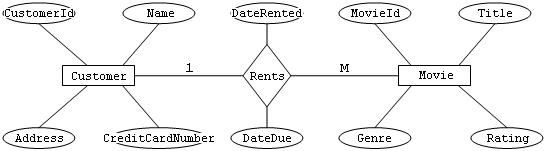
\includegraphics[scale=0.5]{er.png}
\caption{ER图}
\label{database_design}
\end{figure}

ER图用特定的形状来区分数据库的不同部分。矩形表示记录的类型(可以把它看作数据库对象的类)。椭圆表示记录的域(或属性)。菱形表示关系。

虽然ER图中各个元素的位置并不重要,但是认真布置它们,会更易于阅读,而且像Rents这样的关系也可以有自己的属性。

此外还要注意关系连接线上的标签,一边是1,一边是M。这些标号说明了关系的基数约束。基数约束限制了一次可以存在的关系数量。也就是说,基数约束代表的是在ER图中一次可以存在于两个实体间的关系数量。一般的基数关系有三种:

\begin{compactitem}
\item 一对一
\item 一对多
\item 多对多
\end{compactitem}

客户和电影之间的关系是一对多的,也就是说,一位客户可以租借多部电影,但(任何时刻)一部电影却只能被租借给一位客户。基数约束有助于数据库设计者表达关系的细节。


\section{数据库规范化}




\chapter{人工智能}


计算的一个子学科——人工智能(artificial intelligence,AI)向我们展示了计算的未来,计算机发展地更像人类了。另一方面,AI则是应用新技术来解决问题的途径。

AI处理的是人类思想的建模和应用,从普通的到怪异的,AI对许多类型的应用程序的开发都有影响,AI打开了新世界的大门,而这是计算领域的其他子学科做不到的。

AI在采用新技术的应用程序开发中扮演着至关重要的角色。

\section{图灵测试}

1950年,英国数学家Alan Turing发表了一篇具有里程碑性质的论文,其中提出了一个问题:机器能够思考吗?

在慎重地定义了术语智能和思维之后,最终他得出的结论是我们能够创造出可以思考的计算机,但他又提出了另一个问题:如何才能知道何时是成功了呢?

Turing对这个问题的答案叫做图灵测试(turing test),是确定一台机器是否能像人一样思考的衡量方法,图灵测试采用的方式是模拟人类对话。

图灵测试是一种行为方法,根据经验来判断一台计算机是否达到了智能化。这种测试的基础是一台计算机是否能够使人们相信它是另一个人。近年来出现了很多图灵测试的变体。

图灵测试是这样建立的,由一位质问者坐在一个房间中,用计算机终端与另外两个回答者A和B通信。质问者知道一位回答者是人,另一位回答者是计算机,但是不知道究竟哪个是人,哪个是计算机。如下图所示:

\begin{figure}[!ht]
\centering
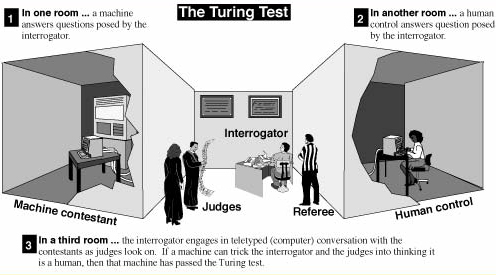
\includegraphics[scale=0.5]{turing_test.png}
\caption{图灵测试}
\label{turing_test}
\end{figure}

质问者分别与回答者A和B交谈之后,质问者要判断出哪个回答者是计算机。这个过程将由多个人反复执行。这个测试的假设是如果计算机能够瞒过足够多人,那么就可以把它看作是智能的。

第一次质问的情形当如此:

\begin{figure}[!h]
\centering
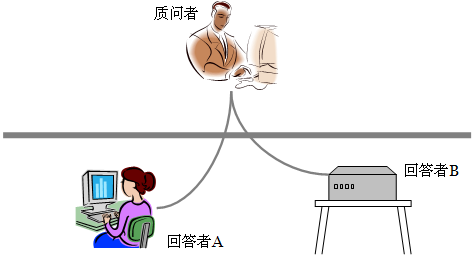
\includegraphics[scale=0.5]{turing_test_example.png}
\caption{第一次质问}
\label{turing_test_example}
\end{figure}

有些人认为图灵测试很适合测试计算机的智能,因为它要求计算机处理各种各样的知识,还要具有处理交谈中的变化所必需的灵活性。要瞒过质问人,计算机需要掌握的不仅仅是事实知识,还要注意人的行为和情绪。

另一些人则认为图灵测试并不能说明计算机理解了交谈的语言,而这一点对真正的智能来说是必需的。他们提出,程序能够模拟语言的内涵,可能足够使计算机通过图灵测试,但只凭这一点并不能说计算机智能化了。

通过图灵测试的计算机具有弱等价性(weak equivalence),即两个系统(人和计算机)在结果(输出)上是等价的,但实现这种结果的方式不同。强等价性(strong equivalence)说明两个系统使用的是相同的内部过程来生成结果。有些AI研究人员断言,只有实现了强等价性(即创造出了能像人一样处理信息的机器)才可能存在真正的人工智能。

这里,弱等价性指两个系统基于结果的等价性,强等价性指的是两个系统基于结果和实现这种结果的处理方法的等价性。

纽约慈善家Hugh Loebner组织了首次正式的图灵测试,Loebner prize成为了图灵测试的正式比赛。

虽然计算机的发展可以使得它们可以绘制复杂的三维图像,处理整个公司的工资表,判断正在建造的大桥是否能承受预计的交通压力。然而要它们理解人类的一个简单的对话却很困难。

人类对关于事物识别等类型的问题具有大量的知识和推理能力,而我们仍然在努力尝试用计算机执行类似人类的推理。

综上所述,在现代技术中,虽然计算机擅长技术,但却不擅长需要智能的任务,AI就是研究对人类思想建模颚应用人类智能的计算机系统的学科。

\section{AI问题的各个方面}



AI学科有很多需要研究的问题,导致现在AI有很多分支,最基本的问题是如何用计算机有效的处理形式表示知识。

目前AI涉及到的主要问题和还未解决的难题大致如下:

\begin{compactitem}
\item 知识表达——用于表示知识,以便计算机能够用来解决智能问题的技术。
\item 专家系统——嵌入人类专家知识的计算机系统。
\item 神经网络——模拟人脑处理的计算机系统。
\item 自然语言处理——处理人类用来交流的语言的难题。
\item 机器人学——关于机器人的研究
\end{compactitem}


\section{知识表达}


表示一个对象或事件所需的知识会根据情况而有所不同。对于要解决的问题,我们需要特定的信息。例如,如果要分析家族关系,那么就要知道Fred是Cathy的父亲,至于Fred是水管工,Cathy有台挖掘机这些信息就无关紧要了。而且我们需要的不仅仅是特定的信息,还需要一种形式,使我们能够有效地检索和处理信息。

表示知识的方法有很多种,可以用自然语言描述知识。例如,可以用一段英文描述一个学生以及他与外界的联系。尽管自然语言的说明性很强,但它不容易处理。所以我们需要形式化的语言,这里用一个近似于数学符号的符号表示学生,这种形式化更适合严格的计算机处理,但却难于理解和正确使用。

从某种程度上讲,AI中也存在数据结构的问题。我们想独立于数据的底层实现,创建它的逻辑视图,以便能用特殊的方式处理数据。不过,在AI领域,我们想捕捉的信息常常会产生有趣的新数据表示法。我们想捕捉的不止是事实,还有它们之间的关系。AI中知识表达要解决的问题的类型决定了要加于数据的结构。

在研究过特定的问题领域后,新的知识表达方法就会出现,比如语义网络和检索树等。




\subsection{语义网络}


语义网络(semantic network)是一种知识表达法,语义网络使用图形化方式表示知识,它捕捉了对象在真实世界中的关系。

语义网络的重点在于表示对象之间的关系。在表示语义网络的有向图中,节点表示对象,节点之间的箭头表示关系。箭号上的标签说明了关系的类型。根据网络图的分析可以回答问题。

语义网络借用了许多面向对象的概念,包括继承和实例化。继承关系说明一个对象是(is-a)另一个对象更具体的版本。实例化(instance-of)是一个真正的对象和这种对象的说明(如对象类)之间的关系。下图展示了一个语义网络,其中既有is-a关系,也有instance-of关系。此外还有其他类型的关系。在语义网络中,关系的类型基本上没有什么限制。


\begin{figure}[!ht]
\centering
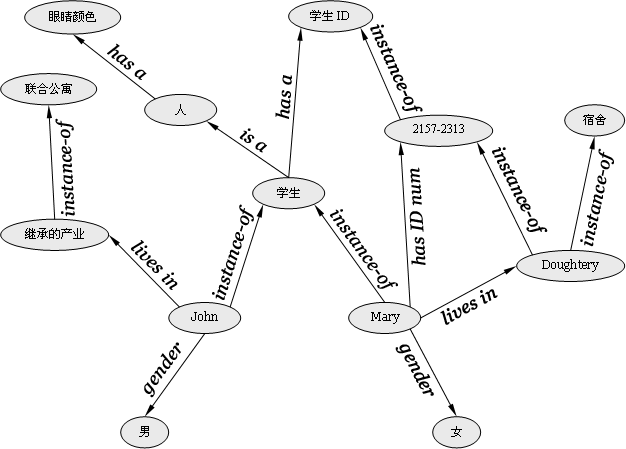
\includegraphics[scale=0.5]{semantic_network.png}
\caption{语义网络}
\label{semantic_network}
\end{figure}

在这个语义网络中还可以表示更多的关系,比如,可以说明每个人是惯用左手还是管用右手,或者说明John的汽车品牌,又或者说明每个学生的成绩。我们要表示的关系完全出于个人的选择,取决于回答我们面对的各种类型的问题所需要的信息。

建立关系的方法也有多种。例如,可以不说明每个学生所住的公寓,而说明每个公寓住了哪些学生。换句话说,可以反转箭头,把lives-in关系改成houses关系。同样地,这种选择也是在设计语义网络时由我们自己决定的。至于哪种方式更适合解决我们的问题,在某些情况下,我们会两者都选用。

语义网络所表示的关系的类型决定了哪些问题是可以轻松解决的,哪些是更难解决的,哪些是不能解决的。例如,用上述所示的语义网络,回答下列问题相当简单:

\begin{compactitem}
\item Mary是学生吗?
\item Mary的性别是什么?
\item Mary住在宿舍还是住在公寓?
\item Mary的学生ID是多少?
\end{compactitem}

但是,回答下面的问题却很困难。

\begin{compactitem}
\item 有多少女生,多少男生?
\item 谁住在Doughery?
\end{compactitem}

上述的语义网络是为表示学生个体与整个世界之间的关系而设计的,其中具有回答这些问题所必需的信息,差别仅仅在信息明显与否。但是如果需要找到所有学生,这里不存在这种信息。

这个语义网络不能回答下列问题,因为它没有表示必需的知识:


\begin{compactitem}
\item John开的是什么牌子的车子?
\item Mary的眼睛是什么颜色的?
\end{compactitem}



虽然已知Mary的眼睛具有一种颜色,因为她是学生,所有学生都是人,而所有人的眼睛都具有特定的颜色,只是根据网络中存储的信息,我们不知道Mary的眼睛究竟是什么颜色的。

语义网络是表示大量信息的强有力而通用的方式,难点在于建立正确的关系模型,用精确完整的数据填充整个网络。


\subsection{检索树}


在数据检索中,二叉树是只有两个、一个或没有子女的树,而一般的树结构的节点可能有多个子女。树在AI中扮演着重要的角色,在对抗性情况(如博弈)中,树用于表示各种可能的选择。

检索树是表示对抗性情况(如博弈)中的所有选择(知识)的结构,例如利用检索树(search tree)可以表示游戏中所有可能的移动(包括你和你的对手移动),可以创建一个游戏程序,最大化它获胜的机会。在某些情况下,甚至可以保证它总是获胜。

在二叉检索树中,只用一个值就可以确定是向右检索还是向左检索。在AI中使用的一般检索树中,一条路径表示玩家的一系列决定。每一层的决定说明了留给下一个玩家的选项。树中的每个节点表示一步移动,这个移动是以游戏中迄今为止已经发生的所有移动为基础的。

下面定义一个简单的Nim游戏作为示例,在这个例子中,一行有一定数量的空格。第一位玩家可以在最左边的一组空格中放入一个、两个或三个X。然后第二个玩家可以紧接着X放入一个、两个或三个O。游戏就这样由两个玩家轮流继续下去。谁把自己的符号放入了最后一个(最右边的)空格,谁就获胜。

下面是Nim游戏的玩法示例,其中使用了9个空格:






\section{专家系统}




\section{神经网络}




\section{自然语言处理}




\section{机器人学}





\chapter{模拟}




\chapter{图形和计算机辅助设计}





\chapter{Embedded System}

嵌入式系统是大型系统中专用于执行有限功能的计算机,嵌入式系统通常嵌在单个微处理器芯片上,程序存储在ROM中。几乎所有具有数字界面的用具都使用了嵌入式系统,如手表、微波炉、VCR和汽车等。

事实上,嵌入式系统无处不在,从电子产品到厨房用具,到汽车,到连网设备,到工业控制系统,处处都有嵌入式系统的应用。

有些嵌入式系统具有操作系统,但是大部分操作系统都是专用的,只需一个程序就可以实现全部的逻辑。

早期的嵌入式系统是独立的8位微处理器,自带操作系统。现在已经发展到32位的数字信号处理器(DSP),到64位的RISC(reduced instruction set,精简指令集)芯片等。而且,越来越多的嵌入式系统开始采用分布式微处理器网络,这种网络可以通过有线或无线的方式通信,由常规的网络管理通信协议远程监管和控制。

而且,事实上,术语嵌入式系统表达的不够清楚,因为它几乎包括除台式PC之外的所有机器。现在这个术语指的是预编译程序来执行大型系统中专门的或有限功能的计算机。其中暗示了终端用户或管理员(如果存在的话)会极少干涉这种系统。

由于一般人只是在厨房、客厅或汽车中遇到嵌入式系统,所以我们才会视嵌入式系统等同于硬件。但是,为嵌入式系统编写程序是必不可少的,而且要把程序烧录到系统附带的ROM(只读内存)中,以便它能够实现自己的作用。

由于不能在嵌入式处理器上开发和测试程序,因此,程序都是先在PC上编写,然后为目标系统进行编译,生成嵌入式系统的处理器能够执行的代码。

在早期的嵌入式系统中,代码的长度和执行速度都非常重要。由于汇编语言能够最有效地简化代码,加速程序的执行,所以汇编语言一直是嵌入式系统的专用语言。即使到C语言出现,并有了跨平台的C编译器后,汇编语言仍然继续被使用。C程序比汇编语言程序大约长和慢25\%,但是比较容易编写。

直到现在,ROM的大小仍然要求代码越短越好,所以汇编语言程序仍在使用。



\chapter{射频识别}


假想一下,我们在商店购买了一块电池,离开商店时,这块电池会“告诉”商店的售卖系统该补货了,因为电池的库存量很少了。射频识别技术(Radio-frequence identification,RFID)就使得这种情况成为可能。

如果给电池包装上安装一个RFID标签,它就能告诉中央射频器自己在哪里。除了应用于零售系统,RFID还用于跟踪货运集装箱、图书馆的藏书、汽车和动物等,人体中也可以植入RFID标签。